\documentclass[11pt]{article}

\usepackage[utf8]{inputenc}
\usepackage{comment}
\usepackage{geometry}

\title{Vision Algorithms for Mobile Robotics\\ (Mini-) Project}

\author{Yvain de Viragh\\Marc Ochsner\\Nico van Duijn}
\date{06.01.2016}

\pagenumbering{arabic}

\geometry{a4paper, margin=1.3cm}

\usepackage[fleqn]{mathtools}
\usepackage{amssymb}
\setlength\parindent{0pt}

\usepackage{isomath}
\newcommand{\mat}{\matrixsym}

% Matlab Plots
\usepackage{pgfplots}
\newlength\figureheight 
\newlength\figurewidth 

\begin{document}
\maketitle
%\pagenumbering{gobble}
%\newpage
\pagenumbering{arabic}


\section{Introduction}
In the process of this course, we implemented several building blocks for a visual odometry pipeline during the exercise sessions. As a mini-project, our task was to put the pieces together and implement a full pipeline. In doing so, we are using some of the work from the exercises as well as some MATLAB functions from the Computer Vision Toolbox. Our final pipeline was tested on three different datasets and showed good performance up to a scale factor.


\section{Pipeline Structure}
\subsection{Initialization}
To initialize the pipeline, we use the normalized 8-point algorithm with RANSAC. We use only the monocular parts of the datasets in order to keep the pipeline as general as possible. Initially, a set of harris corners is detected, described and matched on the first and third image of the dataset. Then the 8-point algorithm in conjunction with RANSAC returns an estimation of the fundamental matrix of the camera. In order to quantify the accuracy of the current guess of F during the RANSAC algorithm, we use the point-to-epipolar-line-distance.\\
\\
After RANSAC has determined the largest set of inliers, the 8-point algorithm is run again on the entire set of inliers. We then use the obtained fundamental matrix to triangulate a set of landmarks using all inlier matches from the harris corner detector. The set of landmarks and key points is now used to initialize the state.

\subsection{Lukas-Kanade Tracker}
Matching harris corners is computationally very costly, as the matching procedure increases quadratically with the number of features. Therefore we decided to use the Lucas-Kanade Tracker on the key points from the previous frame and determine their location in the current frame. 

\subsection{Feature discard}
Features that could not be tracked with the Lucas-Kanade Tracker or were determined to be outliers by the P3P algorithm, are removed by incrementing their corresponding value in a voting array. Once a feature receives more than a certain threshold of votes, it is discarded. This ensures that temporary occlusions caused by moving objects in a scene do not cause complete loss tracking and therefore improves robustness.

\subsection{P3P + RANSAC}
After the location of the features in the new frame has been found, we use the P3P algorithm in a RANSAC loop in order to calculate the current pose of the camera. Again, we increment the “discard” voting array for all key points that have been determined to be outliers by RANSAC.

\subsection{Feature Extraction}
In order to have a good number of landmarks throughout the pipeline, we continuously extract new features. To do so, we extract the harris corners in the current frame, assert that they are a certain minimum distance away from the current key points and include them in our state as candidate key points. Along with the key points, we store the pose during their first respective observation.

\subsection{Linear Triangulation} 
In every iteration, we examine our candidate key points in order to determine whether they can be found in the current frame. If the angle between the bearing vectors of the current observation of the landmark and the first observation is large enough, we triangulate its position and add the feature to the key points in our state.

\subsection{Bonus Features}
\subsubsection{Structure-Only Bundle Adjustment}
In order to increase the accuracy of the pose estimation and to combat scale drift, we run structure-only bundle adjustment on all landmarks which have already been observed a certain number of times. While this will likely not be as effective as full bundle adjustment, it is computationally significantly cheaper.\\
Our approach is based on linear triangulation, but instead of only considering two point correspondences takes in account multiple ones. I.e., given $n$ point correspondences we have the following system of equations:
\begin{equation*}
\underbrace{\begin{bmatrix} p_1^\times \mat{M}_1\\ \vdots \\ p_n^\times \mat{M}_n \end{bmatrix}}_{\mat{A}} \underbrace{\begin{bmatrix} P_W \\ 1 \end{bmatrix}}_{\vec{x}} = 0 \quad \Rightarrow \quad \mat{A} \vec{x} = 0
\end{equation*}
where $\mat{M}_i$ denotes the projection matrix of image $i$ and $p_i = [u,v,1]^T$ are homogeneous pixel coordinates. This linear-least squares problem is solved same as in the case for 2 point correspondences (i.e. using SVD). It is crucial for this approach to exclude any outliers. To this end, we only take into account observations where the reprojection error of the unadjusted landmark is sufficiently small. Furthermore a landmark is only adjusted if it could be tracked for at least 5 frames and we only consider the 10 most recent observations.

\subsubsection{Re-initialization}
We found that for large camera motion, the Lucas-Kanade Tracker would often fail to find the old key points in the new frame. This would mean that we have to either use brute-force matching on all key points, and remove many outliers, which would be very costly. Therefore we decided to re-initialize the entire pipeline with the 8-point algorithm if the number of successfully tracked key points drops below a certain threshold. This is slow and costly, but yields very good results, along with very accurate landmarks which can now be used for a number of frames. Furthermore we found that this procedure alleviates scale drift to a large extent. We achieved good results with a minimum keypoint number of 30. 

During our evaluation, we also tested a procedure where the pipeline regularly re-initializes after a set number of frames. This yields very good results, but slows down the pipeline significantly.

\subsubsection{Custom Dataset Testing}
As an additional bonus feature we made a video in the LFW building of the ETH with a mobile phone camera. To calibrate this camera we used the camera calibration function from the Computer Vision Toolbox in Matlab. The high frame rate of the camera we used lead to small movements between the frames. To overcome this issue and speed up the pipeline, we skipped every other frame. We achieved reasonably accurate results as can be seen in the video.

\section{Parameters and Tuning}
\subsection{RANSAC Iterations}
In the initialization procedure, RANSAC is run in conjunction with the 8-point algorithm. This means we need RANSAC to run long enough such that we have a reasonable chance of selecting 8 inliers in our dataset. By plotting the number of inliers over lots of iterations, we determined that 1000 iterations is a good number to use.

We still found that there occasionally are outlier-matches in this procedure. They are very rare and can only be explained by two falsely matched key points that happen to lie on the same epipolar line. With a large number of inliers this did not affect the performance significantly.

During the P3P pose estimation, we require only 3 points to obtain a pose estimate. Therefore the chances of selecting a sample entirely consisting of inliers is much larger and we found that 80 RANSAC iterations are usually sufficient. However, we received bad results for the parking dataset and chose to increase the number of RANSAC iterations to 500 and received much better results.

\subsection{Harris Patch Size}
During the exercises, we use a harris patch radius of 9 pixels. This showed to be a good compromise for our implementation, as larger patches significantly slow down the pipeline without adding significant improvements in accuracy.

\subsection{Minimum Angle in Linear Triangulation}
When triangulating new landmarks, we ensure that the landmark position is accurate by checking for the angle spanned by the initial and the current observation. The angle depends on the relative motion of the camera as well as the distance to the landmark.
Very large angles proved to be strongly correlated with bad matches as well. We found that by setting a maximum angle, we were able to remove many outliers and achieve much better landmark triangulation. 
For the KITTI dataset we determined that a minimum angle of 1 degree and a maximum angle of 1.8 degrees yield good results. For the “parking” dataset we found that many landmarks are much closer to the camera, so we increased the maximum angle to 6 degrees.

\section{Results and Discussion}
In our pipeline evaluation, we tested the three datasets that were provided with the assignment, as well as our own custom dataset. We also tested with and without bundle adjustment in order to show its effectiveness. Furthermore, we enabled and disabled the continuous re-initialization to illustrate how it alleviates scale drift problems.

Our pipeline was primarily tested and tuned for the KITTI dataset. Figure X shows our custom Z/X plot of the path estimated by our VO pipeline in red, as well as the ground truth provided as part of the dataset in blue. The top image shows the current frame with the successfully tracked key points highlighted with green lines, as well as the candidate key points in blue. The red marks are newly added landmarks. The bottom figure shows the current position with a red cross and the triangulated landmarks with green crosses.

\subsection{KITTI Dataset Comparison}
To compare the performance of our various implementations, we decided to use the KITTI dataset as a benchmark. In this section we will compare four different runs that showcase various trade-offs. First, we discuss our full integration including bundle adjustment and periodic re-initialization. Then we compare it to previous versions of our pipeline, namely with deactivated bundle adjustment, deactivated re-initialization and a combination of the two.

\subsubsection{No Bundle Adjustment, No Periodic Re-initialization}
Figure~\ref{fig:nobanoinit} shows our first working implementation, without the added bundle adjustment or periodic re-initialization. It is apparent that the scale drifts significantly, especially during the time where the car is standing still. Also sharp turns tend to be problematic, and we can see that the pipeline fails almost completely in the top right corner of Figure~\ref{fig:nobanoinit}.

\subsubsection{No Bundle Adjustment, Periodic Re-initialization}
It is clear that our pipeline can only be accurate up to a scale, since we are using monocular images only. The scale is estimated during initialization. This scale can drift as the pipeline advances. It is clear from the graph that the scale only drifts slightly, this is because we are periodically re-initializing to obtain new landmarks.

\subsubsection{Bundle Adjustment, Periodic Re-initialization}
Figure~\ref{fig:bareinit} shows our final implementation's best estimate of the path in red. 



\begin{figure}
	\centering
	\setlength\figureheight{10cm} 
	\setlength\figurewidth{15cm}
	% This file was created by matlab2tikz.
%
%The latest updates can be retrieved from
%  http://www.mathworks.com/matlabcentral/fileexchange/22022-matlab2tikz-matlab2tikz
%where you can also make suggestions and rate matlab2tikz.
%
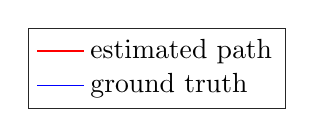
\begin{tikzpicture}

\begin{axis}[%
width=0.951\figurewidth,
height=\figureheight,
at={(0\figurewidth,0\figureheight)},
scale only axis,
xmin=-279.909634132857,
xmax=368.981031803275,
ymin=-17.60491,
ymax=494.181437810917,
axis background/.style={fill=white},
legend style={legend cell align=left, align=left, draw=white!15!black}
]
\addplot [color=red, forget plot]
  table[row sep=crcr]{%
-0.0254918464850879	1.53029535298812\\
-0.0249375910222026	1.94734709129116\\
-0.0603236978857134	2.6546735108884\\
-0.0898810439677802	3.26129873758476\\
-0.122075910018214	3.77863002775995\\
-0.159570842980351	5.84214038823406\\
-0.162924757869628	7.08369056436346\\
-0.345776789656578	7.86663308840249\\
-0.274915939891177	8.64211113562301\\
-0.309598017917685	9.85377995390351\\
-0.277110670012233	10.8074353831107\\
-0.341823185024733	11.5749687633776\\
-0.217611982003351	12.8917266019904\\
-0.0592982609196149	14.535514156623\\
-0.180911942853752	15.86511539354\\
-0.677175153351174	16.7429228811065\\
-1.42757029229411	18.598720661044\\
-1.26066526013012	19.5585825630115\\
-2.09099544665857	21.9137054411806\\
-1.35489091310912	21.6821311104135\\
-2.27343895842534	22.8531216527086\\
-1.72365781744713	23.8629426632053\\
-2.38412979098817	23.3141018626733\\
-2.49982652481565	23.8960769977063\\
-2.64934504463407	25.1017570623487\\
-3.24102646673798	26.8294184308591\\
-2.75227337081859	26.1588342526725\\
-2.25251316649116	26.8675605071435\\
-2.23514914963694	27.9032151877208\\
-2.24609116891217	27.982958602682\\
-2.30118561315577	29.7433987882563\\
-3.41100800227531	31.3865178280425\\
-2.87855773515937	31.9140170643668\\
-3.4368663602838	32.4538719579672\\
-3.11388619330194	33.5688756020074\\
-3.78881356739435	34.4364391121824\\
-4.14043694611709	35.5639350903059\\
-4.24265980636678	36.3360170131273\\
-3.08199500842777	36.2823617856426\\
-3.86218254810391	37.5247117612819\\
-3.78008871169758	38.4796755619529\\
-3.83925339983511	38.9776212507811\\
-3.62251987051958	40.2651303460199\\
-3.72476804662364	40.9917500495216\\
-3.87491538823995	42.1588347214711\\
-4.05345949138225	42.9264327799661\\
-4.55990685408857	43.7076616826611\\
-4.58710434912859	45.1266030356705\\
-4.15662131379484	44.9102241274385\\
-4.32432900127588	46.2011578203503\\
-4.42985739443779	47.0656224658856\\
-4.42962961862714	47.6679605163711\\
-4.57070652957851	48.2221793741606\\
-4.57199673235862	49.4317077831228\\
-4.29788818939738	49.9869788210274\\
-4.3021976565471	50.6767884176887\\
-4.25836254668855	51.4045082969207\\
-3.97410735341543	52.1564613562996\\
-3.52845109049775	52.8879090013884\\
-3.60817948812444	53.2910941672489\\
-4.21767101402003	53.3037102904217\\
-4.26694066421515	53.8252814238761\\
-4.11785254389759	54.1293280041667\\
-4.15707496458134	54.5577610053573\\
-4.41885416695881	54.8395840597333\\
-4.47213079181435	55.2228225873175\\
-4.52586244161301	55.5628903543122\\
-4.66934918726159	55.9017966549809\\
-5.01078860658352	56.2552944315139\\
-4.99428493090294	56.7287729123666\\
-5.02572974611267	57.2588695056402\\
-5.37562191299367	57.7729895574645\\
-5.55237267108766	58.2709251365913\\
-5.44156048501393	58.5639284681207\\
-5.51439869195852	58.9648517597728\\
-5.41642527121364	59.1741555806045\\
-5.60175869371574	59.6963392380832\\
-5.52621049213029	60.0824383205396\\
-5.56512749107208	60.3373151897335\\
-5.65385745413775	60.5368668895362\\
-5.68238964306415	60.7028096755688\\
-5.8506642780277	61.246073230544\\
-5.86068903911556	61.5261630823309\\
-6.0071631450362	61.8201105758982\\
-6.05463522152146	62.2264536916792\\
-6.18359650084802	62.5925169496036\\
-6.16567179398064	62.7721368567187\\
-6.21525354541593	62.9316117983634\\
-6.3728097185946	63.4879041554613\\
-6.3431659748768	63.4859762083145\\
-6.35139809038352	63.6602334297999\\
-6.38096676618425	63.862338851775\\
-6.60340421631325	64.1617853723935\\
-6.47215441417714	64.0923429649715\\
-6.55668332626107	64.3099106129619\\
-6.49413587102935	64.2257225029357\\
-6.48736269570742	64.4231285975602\\
-6.44410730694348	64.5107297521112\\
-6.44742249079286	64.5523797638164\\
-6.46112710882803	64.7596513816304\\
-6.56943486128485	64.9974825541328\\
-5.16228308479518	66.3556355531066\\
-4.73470261263065	66.7887889519573\\
-4.15030439116621	67.4261352053223\\
-3.86240211844175	67.7385412514972\\
-3.44978892931622	68.1035016089998\\
-3.13110621496826	68.1794287485119\\
-2.70805200334046	68.7266136838131\\
-2.7484777951657	68.7613365329827\\
-2.67402025313584	68.7014394323924\\
-2.92527792771013	68.7445552141848\\
-2.7694337810359	68.7533953308252\\
-2.79048689029027	68.7613319033532\\
-2.71623548387942	68.7531223981402\\
-2.64937978216835	68.7662189471711\\
-2.5697465082081	68.7592746391713\\
-2.49264984133266	68.762684434947\\
-2.56442326584954	68.8028874257184\\
-2.42108497972657	68.7452612745006\\
-2.39158148285952	68.7352580976468\\
-2.36767408897901	68.7549506392439\\
-2.31854867713639	68.737357878982\\
-2.25326308040345	68.8030997415243\\
-2.24790489017158	68.8047366095008\\
-2.20922982360595	68.7617953212112\\
-2.11456252891895	68.7041110052127\\
-2.07794541546117	68.7167137088228\\
-2.04011602038262	68.729996900092\\
-1.96444366262119	68.7198340391341\\
-1.90756392847745	68.7372041142033\\
-1.82818010808397	68.7446402253316\\
-1.76544743007254	68.6997819991224\\
-1.69921521961514	68.6844677704676\\
-1.58205436235882	68.6656632810822\\
-1.49136216772553	68.6831456520077\\
-1.4567101931077	68.6608012706501\\
-1.37374816690968	68.633288570018\\
-1.28426654003647	68.6327384078201\\
-1.24221808889874	68.6359465034188\\
-1.1392430160249	68.6203531059414\\
-1.07838210175362	68.6022228751043\\
-1.02353544843056	68.59479665955\\
-0.981007408538902	68.5528204582562\\
-0.880835988977299	68.5492523221916\\
-0.773450073505957	68.5618566392044\\
-0.695800854404705	68.553673402724\\
-0.601504810136044	68.5324317021409\\
-0.466262010668162	68.5166525796782\\
-0.4343579768875	68.493617385709\\
-0.27599634333942	68.5390424448537\\
-0.206137094976174	68.5193363033419\\
-0.166468808423057	68.4977587592106\\
-0.111206330219467	68.4914264680322\\
-0.0417599751618329	68.4921024462819\\
0.0145967346588751	68.4905771615433\\
0.0789563129061079	68.4706575793494\\
0.15111278071101	68.4613257380359\\
0.200445783954544	68.4593257460154\\
0.242432348854578	68.4563843348551\\
0.290143802472025	68.4307018493228\\
0.411268236790518	68.4136438973036\\
0.457033835052604	68.3989872633654\\
0.515167331974428	68.3994790841074\\
0.55311643027307	68.4048832502122\\
0.622834119560803	68.3494574511098\\
0.679235281916124	68.3588114114493\\
0.738647338838874	68.3309205932311\\
0.799304002357957	68.323633803502\\
0.844364545325067	68.319070801932\\
0.874365080037666	68.3206835522439\\
0.92085338499497	68.3050094858578\\
0.970626824519204	68.2933698243747\\
0.994206882684974	68.2800649155739\\
1.06698793905533	68.2668155044703\\
1.12788144409291	68.2437384960775\\
1.19320101142402	68.2319400046377\\
1.17257414431613	68.2258334498327\\
1.22329853867889	68.2110008016179\\
1.24790518322945	68.2001419758047\\
1.28356747582186	68.192860423682\\
1.31970516379937	68.1868566172963\\
1.36855540633614	68.1641922096217\\
1.40072314791968	68.1677282037599\\
1.42956937777001	68.153340480122\\
1.45903301850508	68.1408743154444\\
1.49339510467069	68.1379865518586\\
1.51897631056026	68.133565552244\\
1.54227867288268	68.1319171760544\\
1.59198775263162	68.1274163299167\\
1.61606520743447	68.1245428558043\\
1.64233479578505	68.1243320091555\\
1.67524473461454	68.127474122683\\
1.68890821678942	68.1350127553357\\
1.72532119481408	68.1397308637361\\
1.76040497393434	68.1360895465111\\
2.32637912813648	68.7409965881226\\
2.42557657927692	69.4356487795147\\
2.82984745136007	70.5187103630926\\
4.25243057380952	72.0532863930487\\
4.743631161746	72.7216964925602\\
5.11167469345136	73.3125483069339\\
5.6350054107305	74.231019644157\\
5.89503172952666	74.9362052459969\\
6.32225285236306	76.1189971093224\\
6.7572360405468	76.8696659392275\\
6.90739320692241	77.5698244255377\\
7.49263682144471	78.3555015313727\\
7.84297805349701	80.1064069924676\\
7.99335238523177	80.7065246483307\\
8.39759306420759	81.5202349475433\\
8.65915222013725	81.9493397902011\\
9.16500848676621	83.1967996532794\\
9.45629116759457	83.9375969381233\\
9.63593950681243	85.4815585382871\\
9.88566503644274	85.6315093336213\\
10.2428159132173	86.1265775074272\\
10.7343170245853	87.0828301227972\\
11.0683508107053	87.8736550768478\\
11.1944395496445	88.8970682204383\\
11.4530532318159	89.520605401569\\
11.8186901035052	90.4342172333372\\
12.2614853153901	91.3751535308857\\
12.3749594962316	91.8626890835962\\
12.5739822808096	92.4543697583223\\
12.8979899167476	93.129736020434\\
13.2326878381812	94.4439277313354\\
13.4058288239662	94.5877643227907\\
13.661653488144	95.0940348617212\\
13.903690359268	96.2475913586399\\
14.2988108459682	97.1008676425508\\
14.6077945077504	97.4976415288364\\
14.8958426079441	98.2950626150742\\
15.0074391447246	99.4179952185034\\
15.5491287445354	100.056500746182\\
15.760645617501	100.705357848524\\
16.0128707430768	101.611758095886\\
16.4209885819264	102.656763647934\\
16.7064441880337	103.624969763649\\
16.8700416719813	104.195489666811\\
17.3323404016183	105.746842606074\\
17.1500845522763	104.796547838137\\
17.7342153984745	106.109213751717\\
17.947443290581	106.886431030478\\
18.2432701562009	107.211416478416\\
18.4334315273966	107.397685034675\\
18.492104524037	107.43590895294\\
18.5994569104962	107.43266513871\\
18.9436247371266	108.887253352146\\
19.3043004507618	109.930134967356\\
19.6159352129066	110.296514961295\\
19.9441223687576	110.992038667573\\
20.1482910090224	111.814340931271\\
20.5598264302592	112.083029189193\\
20.9163956134198	113.759018685618\\
21.693339699139	113.787759185057\\
22.1847793331632	115.329250169106\\
22.6089748572092	115.242261070234\\
23.0434764814109	116.589954563773\\
23.6422337305103	117.155429084836\\
23.8547573033722	117.028726449226\\
24.4331179092936	118.199672954091\\
24.9351621109058	118.617531584534\\
25.6625666605772	119.882636912585\\
25.862259517254	120.882595670922\\
26.4710335079412	121.631973416107\\
26.8790165665103	122.068906674435\\
27.6078895609699	123.301606328221\\
27.7610706813634	124.19110486594\\
28.2690748048773	125.090545442458\\
28.9278280044138	125.634671588503\\
29.6680272897553	126.159756389979\\
29.916775241472	126.881179974329\\
30.5104544839036	127.785982831923\\
30.9864693764466	130.070526437571\\
30.8935350423897	131.129137670745\\
31.0059332179696	132.201935583778\\
31.1228205698849	133.52437635679\\
31.3466746411097	134.408331037195\\
31.4038472420089	135.544180746494\\
31.3692358417206	136.681231107119\\
31.5231719314328	138.079832590986\\
31.336375125949	138.355879466341\\
31.4807096726588	139.589486598582\\
31.2574926224906	140.225275633466\\
31.6521669792042	140.932496301322\\
31.4446320210861	141.627832908823\\
31.5284292216924	142.368589669191\\
31.5046296987031	143.305498379961\\
31.8523224522124	144.224733848999\\
31.4315420575404	145.012784307816\\
31.4005452744225	145.761996403217\\
31.3806275046288	146.38775916824\\
31.3225631868471	147.389483403713\\
31.5092562119486	147.925791555093\\
31.5641072238436	148.789220058573\\
31.8288072822233	149.536428548023\\
31.6219988108419	150.314959768323\\
31.6281419965141	151.19917329465\\
31.4316332777911	151.918602352687\\
31.2275407321085	152.58379355785\\
31.2873535146033	153.347962871355\\
31.226682329582	155.211645077753\\
31.2306630352108	156.174631377729\\
30.9564003832906	156.516056708928\\
30.7626843788353	157.385496929875\\
30.8728564574075	158.385369751966\\
30.7663971874074	159.045498570815\\
30.8580800859372	159.841535501677\\
30.7747174099569	160.650241483534\\
30.4952422119895	161.312021792366\\
30.3131850401837	162.263656850787\\
30.1740873299001	162.988327106877\\
29.9877537284804	164.000282832893\\
29.770116234785	165.019585765822\\
29.4097950429042	165.653169318273\\
29.2606187292257	166.544578567415\\
29.1530661213472	167.764357603646\\
29.0036085385588	168.901269796661\\
28.9249761117594	169.998121344367\\
29.0305034055131	170.887919160539\\
29.1108749051132	171.683336623426\\
28.8488903953836	172.583733460536\\
28.8592534591764	173.582579960207\\
28.7564515170669	173.595521113834\\
28.6339041355323	174.307634711422\\
28.5071186672631	175.485720421626\\
28.3739764649885	175.613968442466\\
28.4258538529184	176.407227632034\\
27.8055077526936	178.182678071383\\
27.6028273177362	180.071426595132\\
27.6706284214983	181.393143065044\\
27.5714094736419	182.378457465733\\
27.3345962035589	184.297725437826\\
27.2050946893493	184.852792513314\\
27.0273970903181	185.80953423445\\
27.0696777142104	186.367454987379\\
26.8790358027877	187.070788115954\\
26.835616545771	187.872250955736\\
26.6688072627824	188.479385263934\\
26.451423500193	189.103604111808\\
26.2099976579884	190.008257479677\\
25.8936463365625	190.723665157023\\
26.0214872958566	191.41048176177\\
25.9223815739118	192.072325809546\\
25.8885468322707	192.556858431119\\
25.655178520461	193.488491817572\\
25.6041712223397	194.096876321591\\
25.5542120919866	194.859843310874\\
25.6147810425441	195.267942561724\\
25.7964288253991	195.616738472469\\
25.634793202666	196.427482122492\\
25.8194364080329	196.669795839361\\
25.6930298943844	196.934463548948\\
25.8560220238842	197.586265492008\\
25.7443452290368	197.880702781958\\
25.7050015472644	198.162392567377\\
25.45264865354	198.916789034969\\
25.5216566400808	199.47729416911\\
25.39486818651	199.8917475016\\
25.3823838189762	200.430621275378\\
25.3918465236732	200.805200354695\\
25.3714867622897	201.125521219416\\
25.336604991804	201.759935573005\\
25.2412254219563	201.776461977076\\
25.2283632089339	202.028639766291\\
25.1993337604282	202.26625898985\\
25.2115271331007	202.544861450753\\
25.2127826740648	202.820300479003\\
25.1417397075799	203.120935105433\\
25.1286994092587	203.34223235254\\
25.1608137399525	203.63104704152\\
24.8645712183388	203.961310126502\\
24.7865644352517	204.346462328168\\
24.7695377621816	204.667691677212\\
24.8122071734759	204.929472113458\\
24.7344360646849	205.356025866679\\
24.7313817895402	205.545961284727\\
24.6216376080747	205.919818508193\\
24.5361418913689	206.285323902868\\
24.5262873359962	206.619266792245\\
24.4280411379531	206.93297503833\\
24.4868197675078	207.23352721783\\
24.3620964141778	207.532373922107\\
24.3443266644148	207.923351840319\\
24.2899831134889	208.302867722769\\
24.2056541730923	208.620881532893\\
24.2671794104946	208.830538705943\\
24.2256210632622	209.097985126339\\
24.1635833921456	209.431120865591\\
24.2233287801773	209.753566667915\\
24.2245059323107	209.975924755926\\
24.2773876722535	210.0280206528\\
24.2153841830566	210.339243146341\\
24.1471369166393	210.554585854975\\
24.123640650444	210.808817936811\\
24.0231940665651	211.092799675821\\
23.9991855615781	211.255022307387\\
24.296872806854	211.092929051617\\
23.9822441068207	211.527249206175\\
23.9663092023658	211.509639175926\\
23.9846432853858	211.347632540596\\
24.0325470142418	211.349196736734\\
24.0407842533872	211.356997105029\\
24.0190527441633	211.210934216378\\
23.777087003753	211.686636966901\\
23.6290913503958	211.754922423789\\
23.347617750422	211.315916522719\\
22.2524627030443	211.293173409533\\
21.73124023025	211.621101209519\\
22.2464970002914	212.042059997957\\
22.7313425290074	212.08134723709\\
23.0354084648533	212.123513276966\\
21.4134480282015	212.589471750404\\
19.7979307066517	212.913217797488\\
19.2582905686774	212.884911382348\\
19.1678545763804	212.647773213406\\
18.2483010946474	213.308255642926\\
18.1497635544864	213.482520091896\\
17.5661112332419	213.846523682728\\
16.6291258037731	214.27415240985\\
15.4157968044397	214.186375980845\\
15.3663427688224	214.233570425831\\
14.9142040393703	214.076332603915\\
14.5382827027154	214.013088263563\\
13.4904734289621	214.626781031759\\
13.0930353529109	214.357473836844\\
12.1321476337684	215.038762249081\\
12.0048455141304	214.479461964732\\
11.5166877275124	214.343992242921\\
11.2594441579004	214.365571889851\\
10.875476560048	214.586743906002\\
10.5620231890785	214.345061005698\\
9.67465674002987	214.495829507906\\
9.29944832590777	214.554881514925\\
8.80139367164341	214.798070626697\\
8.08093368817823	214.857404698567\\
7.55624547608903	215.125308174891\\
7.33934871340871	214.867432865852\\
6.81292613526508	214.712556664222\\
6.23647880029449	214.854215357086\\
5.93709101155725	214.638949301433\\
5.11450982724467	214.83853329361\\
4.53934808805743	214.796327079969\\
4.10356983637135	214.930740172533\\
3.54342325576398	214.750326372446\\
2.91900538966626	214.855105243567\\
1.92114104206102	215.036547880958\\
1.83017110963159	214.844064685131\\
1.13166415742217	214.991768665409\\
0.795647525566089	214.914248164717\\
0.423140774757908	214.864776410601\\
0.589737107243323	214.769381925329\\
0.393611465711487	214.691793442922\\
-0.319356415268118	214.869781348428\\
-0.395886850728132	214.679808906286\\
-0.926122499699243	214.722523351686\\
-1.07053173999774	214.666469876697\\
-1.267531205691	214.605705001317\\
-1.59833670719756	214.555592137776\\
-2.18928151947033	214.669281051706\\
-2.45883827287967	214.657249576627\\
-2.61299595524665	214.593288620563\\
-3.10517987313153	214.722375792856\\
-3.32237209041765	214.63695728217\\
-3.61088863411375	214.569154220346\\
-3.79532226882941	214.538822254458\\
-4.10453752687978	214.512243612151\\
-4.51906713964134	214.447003648654\\
-4.77442366364141	214.422729982806\\
-5.13341990484228	214.424987260822\\
-5.33751944152229	214.304420156075\\
-5.69933848586392	214.310484343659\\
-5.82938422985549	214.205648373489\\
-5.97607562187358	214.23161507837\\
-6.08421126276354	214.141095761368\\
-6.19156477763469	214.148061810589\\
-6.35516108177956	214.027083039427\\
-6.79278687489574	214.158843240963\\
-8.88470477438872	214.00388554744\\
-9.5602040296985	213.497422675691\\
-10.3436532243474	213.573031472916\\
-11.2414652349485	213.462680855285\\
-12.047769715407	213.156959254144\\
-13.2342075482977	213.225157546666\\
-14.3577549505562	213.210457570065\\
-15.2708107054786	213.144543970133\\
-15.7291004810213	213.034415470773\\
-16.704549727583	212.951822592387\\
-17.3808564994151	212.637022189031\\
-18.7991388507424	212.966865047599\\
-19.0953427731673	212.861572662411\\
-19.3619714962359	212.479895910625\\
-19.9376331202177	212.416179263601\\
-20.4622915085327	212.382166887641\\
-21.2685842433885	212.277015414084\\
-22.1354251151204	212.434877366505\\
-22.7481600732877	212.597266370167\\
-23.7113121286454	212.809241576281\\
-24.572830829869	212.474581741946\\
-25.0057571871728	212.618232136984\\
-25.7452986609307	212.618093541893\\
-26.4145191978103	212.66790332991\\
-26.7471187596246	212.721332620844\\
-27.5497642389168	212.883190508485\\
-28.0450254576246	212.815482437103\\
-28.4263283425603	212.856750314121\\
-28.8520835568439	212.837988969263\\
-29.2247156330257	212.689012106691\\
-29.7583753912387	212.904208868114\\
-30.2091977104723	212.815413466712\\
-30.5946019859669	212.908389382693\\
-30.8303034923719	212.92234164273\\
-31.1790803695378	212.820781076697\\
-31.4784184690701	212.904773760019\\
-31.4049760659972	212.934092025406\\
-31.6080873367598	212.935297227569\\
-31.7384907553753	212.851716191155\\
-31.8898459052867	212.818220024182\\
-31.9638974764624	212.829094001591\\
-32.1824879928357	212.98841687425\\
-32.1655223170709	212.840021572307\\
-32.1923908149378	212.9172267565\\
-32.0916810749162	212.91030020718\\
-32.1489909083316	212.896514607043\\
-32.15964305121	212.942742021821\\
-32.2000980408644	212.904409072289\\
-32.1926832969525	212.914999300785\\
-32.1489311833243	212.928029674289\\
-32.1417631721691	212.929110146895\\
-32.1752900774627	212.941440586801\\
-32.1215717355744	212.923694104363\\
-32.2254422252891	212.898680008697\\
-32.099820638685	212.918205505977\\
-32.3012840382865	212.849441959141\\
-32.2401240422764	212.892675756026\\
-32.1059648103308	212.898156761293\\
-32.2187080066856	212.857117284202\\
-32.2849660052344	212.91479898346\\
-32.3053575615531	212.896996909545\\
-32.3908949545142	212.916195285458\\
-32.3691386656538	212.913586729109\\
-32.4840201353643	212.862941086131\\
-32.6233134103869	212.858265977824\\
-32.7068969515437	212.888763395313\\
-33.2174837373732	212.945253061197\\
-33.4373042866178	212.80362060497\\
-33.5662675146952	212.854121105593\\
-33.918576969566	212.956682674868\\
-34.1750611501107	212.900609851177\\
-34.3050970169915	212.980494311042\\
-34.7591335306888	213.230402599525\\
-35.0133240475871	213.110161487189\\
-35.1027949518492	213.062289142315\\
-35.3856731622133	213.273421391619\\
-35.4886092932079	213.301003918611\\
-35.9353010442333	213.344452939839\\
-36.0205759616671	213.552351596785\\
-36.4321499581096	213.6355438708\\
-36.6630331594686	213.698629205214\\
-37.4571198298805	213.987346099098\\
-37.5561187478809	214.18551884902\\
-38.030548384609	214.461430410488\\
-38.2360149590335	214.659015176915\\
-38.7131687933331	214.886831225974\\
-39.2365113985385	215.257630458455\\
-39.4370799656358	215.689444867075\\
-39.5503623257288	216.027016510892\\
-39.7905470537138	216.326888932857\\
-40.252653846781	216.84613291881\\
-40.3111508848086	217.432588396869\\
-40.6156984536395	217.744486044755\\
-40.8473865542094	218.319065934572\\
-41.0893217248059	218.674494817595\\
-41.0774102378002	218.742966840269\\
-41.5222631015515	219.802071979507\\
-41.7411348174162	220.217207900609\\
-42.2345021377749	220.998391819105\\
-42.5176819356347	221.431961240657\\
-42.8592816956743	221.827565468201\\
-43.5110475720288	222.853237577047\\
-43.9224051734094	223.83577780191\\
-44.0229368417564	224.787218372985\\
-44.3259876952366	225.739007947086\\
-44.2861194606393	226.237304108418\\
-44.6137712157757	226.237631739993\\
-44.7091554419576	226.576856364125\\
-44.7116951785624	227.287873256857\\
-44.8423914174883	227.625587539739\\
-44.6970852206428	228.047112811744\\
-44.7059763403861	228.228507053352\\
-44.8908655809168	228.910411746398\\
-44.9740871271561	229.374442034491\\
-45.1344783697858	229.934920204791\\
-45.2212898538476	230.417483410399\\
-45.3790843504595	230.928079585211\\
-45.4206004797457	231.224953745021\\
-45.4308381858286	231.736006403963\\
-45.3300060452855	231.700480568538\\
-45.7891901579862	232.251789804872\\
-45.84726280253	232.607707089245\\
-45.9257479418923	232.874296094355\\
-46.0917299313781	233.636686653868\\
-46.2203703593597	234.247682205506\\
-46.3094706964418	234.683288644602\\
-46.4473023338355	234.973072461477\\
-46.5603347315074	235.262463892118\\
-46.6431314821818	235.719033916002\\
-46.7226948076352	236.113304962719\\
-46.8161031493154	236.445965880473\\
-46.9075886961262	236.672789912754\\
-47.081739943149	237.488090828786\\
-47.2010674183691	237.809628867081\\
-47.246512765219	238.505143654282\\
-47.1473131458185	240.441319121648\\
-47.2324589011008	241.361301522648\\
-47.422539945568	242.086540900497\\
-47.1548958910591	243.341582853407\\
-47.1247005117633	243.989390924863\\
-47.0963491584297	244.828805920311\\
-47.0224336947515	245.626737679853\\
-47.0501833043112	246.700490314079\\
-46.9542678656876	247.346715397458\\
-46.8739159753082	247.977698935206\\
-47.3139505715168	248.514304708373\\
-47.5031451145017	249.383264734853\\
-47.6894072119365	249.605704301269\\
-47.9822090892648	250.326250440796\\
-48.1930909511224	251.381780851603\\
-47.683497608932	253.346961566476\\
-47.1437025965653	255.269188919135\\
-46.9555399297772	255.728788855105\\
-46.9113871215947	257.540988819626\\
-46.4018998531305	258.215020825359\\
-46.1691399624514	259.169708499103\\
-46.0006329777693	260.144908009681\\
-45.4942496213327	260.861282448583\\
-45.1837996456915	261.695799310811\\
-44.8439308560947	262.945669476523\\
-45.031056448566	263.445196847028\\
-44.6051055468825	264.644878476725\\
-44.5375296457634	265.52298933947\\
-43.9379023975452	266.734832466098\\
-43.7761271905091	267.611227603413\\
-43.2437162313124	268.112421714943\\
-43.3574505322155	269.036962788332\\
-42.8119051592064	269.969030602106\\
-42.6380071422129	270.653681792449\\
-42.8539840160955	271.25007885561\\
-42.430597124949	272.125926734298\\
-42.1451730155138	273.102027691711\\
-41.8563532834494	274.087495671695\\
-41.2968953440232	274.936185282528\\
-41.2225874507555	275.917660109676\\
-40.8923722906232	276.749409408474\\
-40.6038548602881	277.849571215356\\
-40.1537628651525	278.480987491248\\
-39.8130405265665	279.481478060277\\
-39.4631222518126	280.37412522484\\
-39.0252560389229	281.084480035055\\
-38.2881664842881	282.380661662572\\
-37.8950494319854	283.199695717622\\
-37.4156696292089	285.377285892079\\
-37.1246989925732	286.567755242813\\
-37.0078289946857	287.759353528826\\
-36.4235674532139	288.655128827211\\
-36.4206719222769	289.479169194261\\
-36.0199877742188	291.388416932704\\
-35.7371574949692	292.287462651489\\
-35.4944568807212	293.428513242332\\
-35.0724434707039	295.326881637912\\
-34.9267090809202	296.357985976457\\
-34.7962987803007	297.304945783259\\
-34.6677445856661	298.406750037939\\
-34.4175366530386	299.203530674089\\
-34.2497002644438	300.050480234458\\
-34.025015461553	300.846638483316\\
-33.9052652051478	302.057645773539\\
-33.8262493158549	302.886600286682\\
-33.5523434137671	303.928982136653\\
-33.0947880894399	304.839200182004\\
-33.435879549583	305.517276228189\\
-33.0356890527176	306.281694684402\\
-32.9853019988319	307.248799760557\\
-32.9544689753232	307.927088377347\\
-32.220810070766	309.150152962646\\
-32.1525551845704	309.759636242243\\
-32.9989570805084	309.915338106239\\
-33.4321504999133	310.186200619098\\
-32.9836081768361	310.905274657959\\
-32.5750584820784	311.665455473466\\
-32.0190359696176	312.814504882672\\
-31.4700124082084	313.798267948704\\
-31.0882394843671	314.232613800771\\
-32.6048323084808	314.979950582979\\
-30.4822555189457	315.811317736442\\
-31.0292626567009	316.382484300536\\
-30.9310114462225	316.87814082286\\
-30.6864767041683	317.886727392411\\
-30.7726610461201	318.993196905374\\
-29.0576603098639	319.798787959842\\
-28.7711605010995	320.623311392259\\
-28.7093404830653	321.259517703079\\
-28.9041161327918	321.972302837225\\
-29.0941573601318	322.771694921716\\
-29.0994113613896	323.675771526195\\
-29.0885143088973	323.429907778961\\
-29.3428586520038	323.795665938011\\
-30.0541236364524	324.06992945094\\
-30.0695284081772	324.524674301971\\
-30.0250587285471	323.99094762543\\
-30.0815687814954	324.407852889984\\
-30.2664215409223	325.061368068208\\
-30.5387720312818	324.548372508383\\
-29.8153167473754	324.460218777784\\
-30.2202994195	324.812651250332\\
-29.9255936919935	324.4731767891\\
-30.2564989140735	324.809243384898\\
-30.2160583559844	325.045066532158\\
-31.9520686894934	326.035155722726\\
-32.6222818170176	326.559188293965\\
-33.2138329306937	326.536234127881\\
-34.7489286227544	327.291839472857\\
-35.8494644332291	327.531403381621\\
-37.083633031998	328.035070118398\\
-38.6536244031342	328.859228715703\\
-39.4408761340687	328.729092545352\\
-40.6655524623809	329.318066798766\\
-42.1020469335577	329.677156840239\\
-44.2040416163879	329.612365954592\\
-45.6794767154268	329.868795854747\\
-46.7064011268461	329.546411286154\\
-48.614928246103	329.378190940468\\
-49.9309875262262	329.635189708725\\
-51.3563823558072	329.723357193928\\
-51.0978106620835	329.908610425922\\
-52.2001043527608	329.790119639989\\
-53.877185604255	329.556497371619\\
-55.036841966622	329.621806594873\\
-56.495076964268	329.946714257879\\
-58.0801408344746	330.254718163287\\
-60.059959450994	330.300764588298\\
-61.2911627109869	330.101095233726\\
-61.8985535743654	330.214282061376\\
-63.0434713996976	330.21308547089\\
-64.5674860363518	330.209961250284\\
-64.571133956562	330.349796581707\\
-66.252740907551	330.426465380046\\
-67.3101021438173	330.507246990496\\
-69.3443083489517	330.711530451238\\
-70.4757133828234	330.589493937085\\
-71.6656722855487	330.544071468239\\
-72.4464422085937	330.784337440676\\
-74.3395275300129	330.883615340343\\
-75.3250730270993	330.95899134696\\
-75.9760534680185	330.949121200304\\
-77.4039667771099	330.826729931524\\
-77.9830187850089	331.000247864272\\
-78.8687689456271	330.936635887811\\
-80.2344578369083	331.277002425432\\
-81.4185828783275	331.180546591004\\
-82.1579831466836	331.255430568315\\
-84.2701165695666	331.331188785134\\
-85.381765018527	331.328927260221\\
-85.9187303825449	331.342604183633\\
-86.0058085659101	331.596210159356\\
-86.6345463070181	331.704106100662\\
-87.1532675488185	331.573066087587\\
-87.8758778539771	331.949890100947\\
-88.5495553098208	332.12871940584\\
-89.0586796220371	332.069320924164\\
-89.395828767759	332.256034299604\\
-90.3906163926342	332.250450270316\\
-90.6364606915531	332.613369771351\\
-91.2923595527582	332.826427360494\\
-91.6158289510457	332.932953700456\\
-92.3925204689356	332.926229695809\\
-92.6201219071659	333.050243107929\\
-93.6608464832948	333.26887947839\\
-94.4564065706272	333.391609558434\\
-94.9726830240708	333.31261823923\\
-95.3938220813347	333.471138520326\\
-96.0267459745488	333.776066349316\\
-96.4667262182685	334.09191598723\\
-96.8006882772589	334.344229082932\\
-97.7038509323724	334.315042074222\\
-98.2508769633903	334.332510376898\\
-98.4998469680749	334.608676587533\\
-99.0010742313726	334.460400574565\\
-99.3772112309244	334.87542186045\\
-99.8433775263427	334.969477408754\\
-100.369196958569	334.816270984674\\
-100.649054809036	335.144544991477\\
-100.884502098649	335.11477631906\\
-101.399073744781	335.147006853795\\
-101.655398223972	335.214153157286\\
-101.943192743224	335.139046799433\\
-102.246850048485	335.400610178079\\
-102.490391100558	335.302013711441\\
-102.959386146335	335.335032828147\\
-103.235184130284	335.159673109969\\
-103.533272683701	335.167071109366\\
-103.787873027846	335.10828616072\\
-104.177976753419	335.076443599708\\
-104.442229917373	334.932458772789\\
-104.69957459767	334.820706066122\\
-104.95390297583	334.646222726798\\
-105.442052158665	334.784885639064\\
-105.523430740352	334.648393119687\\
-106.162055256026	334.685078637888\\
-106.419529930642	334.73982636409\\
-106.740111361581	334.679535636641\\
-107.013001576927	334.527776532129\\
-107.29244961418	334.487849615371\\
-107.717829637576	334.354699620496\\
-108.015942696537	334.306738033252\\
-107.973778380001	333.982257556483\\
-108.400981083681	334.04631437748\\
-108.877448657914	334.029644085789\\
-109.67857339769	334.185142370678\\
-110.116884349427	334.087659682204\\
-111.90624992421	333.515256346859\\
-112.879919763106	333.268432338534\\
-113.733477980254	333.152697204073\\
-114.477870675761	333.280187897946\\
-115.134794276	333.362493838527\\
-116.29925573759	333.279273206963\\
-116.592195632737	333.099436641115\\
-117.4469544453	333.255064924585\\
-118.311459427027	333.266768218191\\
-119.142995658145	333.386375393761\\
-119.5519804159	333.143294097204\\
-120.125727095054	333.229007628851\\
-120.599301493847	332.917557923802\\
-121.41050654491	332.941315350844\\
-122.010740708945	332.683071914598\\
-122.448065444772	332.740223493192\\
-122.737659238848	332.506115198567\\
-123.319242686169	332.37173759706\\
-123.987170959506	332.216396772916\\
-124.699999564765	332.094822017949\\
-125.300055595285	332.14542450167\\
-125.832855582729	331.940284959672\\
-126.279710584852	331.882406939749\\
-127.204212105544	331.740714442927\\
-127.437097449713	331.582905914604\\
-128.047247777049	331.428515154805\\
-129.876237550654	330.829171331589\\
-130.675736570094	330.567752334914\\
-131.570550603339	330.320907279621\\
-132.496049348151	330.14786487886\\
-133.884600251746	330.225623704696\\
-135.147411479847	330.029604868238\\
-136.572718042015	329.845383755894\\
-137.396388652978	329.775610094747\\
-137.918188575155	329.630338461391\\
-138.941678383965	329.541154961344\\
-139.627816168456	329.505438319312\\
-140.279651442428	329.345139677669\\
-141.792467729002	328.383745769038\\
-142.483116797835	328.030731515725\\
-143.797691730101	327.331695780086\\
-144.652175696273	327.009717122671\\
-145.173094563113	326.707886081164\\
-145.460328039472	326.441495551787\\
-146.246866769475	326.146609899088\\
-146.668040309708	326.000219841559\\
-147.321275893584	325.777797065317\\
-147.683129388003	325.488427994554\\
-148.195929444065	325.364505374244\\
-148.365987947546	325.059133930781\\
-148.826378158346	324.919332220775\\
-149.467056581452	324.542590690758\\
-149.761458285886	324.45875226042\\
-150.238774904033	324.208785529118\\
-150.65551674814	323.969433938326\\
-151.12117195531	323.723785882836\\
-151.438736664022	323.540682132909\\
-151.964496223281	323.240518656497\\
-152.316078225546	323.020792357025\\
-153.04437643066	322.859905288161\\
-154.031536232429	322.709983758657\\
-153.972702827433	322.666683382184\\
-154.829604253641	322.337053066111\\
-155.390334144188	322.166804669758\\
-155.880416335035	321.984899150535\\
-156.193162072909	321.739684416764\\
-156.434391946001	321.838273864625\\
-156.515287540772	321.654037114348\\
-157.010276722406	321.527434897005\\
-157.244448124897	321.48013903531\\
-157.921143964233	321.283412530287\\
-157.861556455003	321.263850761104\\
-158.130419362393	321.124020948531\\
-158.131966355271	321.159737586622\\
-158.548488606006	321.015362563419\\
-158.657462295401	320.880857157309\\
-158.825540420148	320.732333686745\\
-158.955732436493	320.628360019961\\
-159.178561595351	320.545081654653\\
-159.137506761558	320.408073940571\\
-159.281509093168	320.269489058068\\
-159.317908848195	320.210843154201\\
-160.478123333959	318.682124414268\\
-161.139149377988	317.936759801109\\
-161.762842249052	317.164990636701\\
-162.110243690989	316.516665543159\\
-162.52246555518	315.78798297121\\
-163.062406545729	314.959480615909\\
-163.36841871443	314.069741823325\\
-163.84157453904	312.945700811698\\
-164.125975728303	312.071284641597\\
-164.140790938608	311.083827897955\\
-164.279777171775	309.839777746885\\
-164.343833241378	308.647649292341\\
-164.186305185735	306.865603735224\\
-163.995485104298	305.960997473035\\
-163.706813591252	304.762266819116\\
-163.443236858023	303.961943434836\\
-163.073334575185	303.037218830003\\
-162.893968706577	301.846702938645\\
-162.453733030198	301.98118062225\\
-161.945187393466	300.101071588761\\
-161.371514143463	299.053694251175\\
-160.827866204798	298.321290425909\\
-160.330812957109	297.210046610852\\
-159.667563143266	295.91291712907\\
-159.42085689736	295.044964649416\\
-158.685275431209	294.076498536341\\
-158.003239755802	292.939114291171\\
-157.195822664636	292.116352439604\\
-156.458618996731	291.031245088548\\
-155.906508685092	289.77029679907\\
-155.302381485757	288.593407172014\\
-154.612518173298	286.736373934322\\
-153.654644306031	285.359951882782\\
-152.869442229504	284.247597224703\\
-151.827803967904	281.754028007394\\
-151.526621427761	281.041748466778\\
-151.178431861716	280.608913003979\\
-150.118116967703	278.967105665674\\
-149.179948801558	277.677277777835\\
-148.382289422446	276.271825353436\\
-148.308353859261	275.841838271823\\
-147.382082786506	274.477561840411\\
-148.701861557453	276.810385262411\\
-147.516611222775	275.280778142688\\
-147.447680232126	275.188704910755\\
-150.216350228997	280.442435026993\\
-148.20238660051	276.611991877723\\
-149.87651367536	279.785975326546\\
-148.162880418572	276.521631287993\\
-147.650088969941	275.653563070944\\
-147.245207925049	274.976395244904\\
-146.962935673125	274.870291855785\\
-146.677110387634	274.273976595519\\
-146.580182570659	274.051283609348\\
-145.509545152285	272.342277072142\\
-145.322228176124	272.094377008742\\
-144.945979234247	271.408236692924\\
-144.554018470191	270.729447618948\\
-144.253056423026	270.057205719845\\
-143.651365829514	269.337852022637\\
-143.218274327141	268.665739075668\\
-142.71901748183	267.404175120123\\
-141.894204841188	265.916096219827\\
-141.487614773499	265.390816477406\\
-140.984725677432	264.209064867018\\
-140.678517160559	263.669532829174\\
-140.309669096227	263.601171155133\\
-139.921313183609	262.665604056736\\
-139.590439571805	262.159519473578\\
-139.096955313929	261.092651409541\\
-138.669279586481	260.69430810209\\
-138.336281870439	259.752111525286\\
-137.842361570881	259.087098850233\\
-137.716499454746	258.970251979528\\
-136.987711877504	257.512765282397\\
-136.861372730202	257.41308765526\\
-136.500815231841	256.841158187767\\
-135.980077189174	255.802388581903\\
-135.515623623764	255.207893920101\\
-135.9727456844	255.813062986686\\
-135.519564604397	254.84212019283\\
-134.864447639659	253.851226745538\\
-134.961930039505	253.940134672072\\
-134.150642897339	252.748892888294\\
-133.864201088266	251.896083236671\\
-133.446718707118	250.965095389099\\
-133.351077061694	251.057419907868\\
-132.973454709031	250.49651104699\\
-132.52299734229	250.183263796926\\
-132.520986557355	249.977793520293\\
-132.160058587118	249.300985879901\\
-131.713870505367	248.271346774854\\
-131.597538668984	247.620761751135\\
-130.566781641153	245.993766030124\\
-130.086487549233	244.971618427715\\
-128.951382644766	243.351862263987\\
-128.684353313651	242.380190829467\\
-128.042306670538	241.687840524302\\
-127.377483604256	240.604362171387\\
-126.850945730886	239.785445963307\\
-126.590827341515	239.463132346264\\
-126.468795866327	238.47528061406\\
-126.257829563609	237.801992715139\\
-125.955898131242	237.775355588748\\
-125.76909113202	237.556991367827\\
-124.865440512175	236.277201310559\\
-124.660949829503	235.845050891949\\
-124.159374602776	235.131691099976\\
-123.837422815175	234.669079334305\\
-123.392708424975	233.854213616925\\
-122.938407607964	233.38669157015\\
-122.871606611568	233.071594093442\\
-122.486716391935	232.656675830372\\
-121.99745902045	232.078049924719\\
-121.774453390392	231.7412042619\\
-121.678388180141	231.633083746823\\
-121.514193268524	231.241640729135\\
-121.417872547082	231.156181969279\\
-121.181040437177	230.773897908064\\
-120.990345802502	230.713139606059\\
-120.787522819944	230.462451969444\\
-120.360000034531	229.917547354534\\
-119.445583253479	228.107825923055\\
-118.834480188413	227.315846331024\\
-118.572692925967	226.732379749929\\
-117.953649265625	225.694646338897\\
-117.544887581961	224.997139328139\\
-117.074177504166	224.186357510038\\
-116.669850208607	223.420507055236\\
-116.273713145253	222.543354617546\\
-116.135368281281	221.599131819992\\
-115.420076516011	220.74402672682\\
-114.978457216216	219.950358764528\\
-114.776907997416	219.797845072677\\
-114.358922470469	219.35912293991\\
-114.025977289443	218.847075497957\\
-114.277030599945	219.297708309212\\
-114.08317563492	218.908473361187\\
-113.249146029026	217.720604563909\\
-113.394792632991	218.052096876042\\
-112.795949113259	217.106874757422\\
-112.405417467161	216.639946234222\\
-112.721458325405	216.912800415849\\
-112.419196926301	216.951582108379\\
-112.163897234046	216.251299697696\\
-112.001078678595	216.018113129349\\
-112.192585474409	216.554714746711\\
-111.812552145166	215.96746455893\\
-111.659085442292	215.745802277594\\
-111.451047654751	215.195416916847\\
-111.132928430401	215.108883749112\\
-111.449659971089	215.244084071734\\
-111.297808454811	215.035089791567\\
-111.024805527011	214.716939466218\\
-111.49980164705	215.529276272836\\
-109.572304061658	213.235374556756\\
-109.994409556547	213.462300704725\\
-110.029073757718	213.57002939415\\
-109.773247755018	213.164481682024\\
-109.923747835861	213.696414914563\\
-110.251920962686	213.63926276724\\
-109.893214623728	213.549222910212\\
-109.56194253279	213.122942593999\\
-109.441677642589	212.833142135002\\
-109.612121959644	213.024450877088\\
-109.212737491224	212.628729607687\\
-109.185918727802	212.665360885028\\
-108.909931556552	212.085629602279\\
-108.787745645936	211.900715429195\\
-108.547274841134	211.520414553145\\
-108.417439680511	211.325244866368\\
-108.371655036158	211.476523646937\\
-108.271054181033	211.261759045497\\
-108.08089267768	211.045279754551\\
-107.906530439696	210.950615623151\\
-107.721330400231	210.698921934264\\
-107.374903490384	209.662736336646\\
-107.103999133254	209.588875110793\\
-106.74548561882	209.208855677645\\
-105.224859791315	208.587962695366\\
-104.05874586137	208.426876997512\\
-102.3019750021	208.204520867129\\
-101.690301389833	207.917901188845\\
-100.496092898887	207.866152965114\\
-99.6569123689388	207.87112066118\\
-98.1766083932973	207.937036546367\\
-96.6622712473059	207.911564218157\\
-96.0221629205822	208.111966499001\\
-94.8055045935807	208.301723638191\\
-93.9335893604707	208.560133691434\\
-93.316072705585	208.97019171986\\
-91.6323436607293	209.698515553391\\
-91.2604674250002	209.620763147314\\
-90.0305874742968	210.245570871478\\
-88.8340311361344	210.729518487423\\
-88.1160090061757	211.167816922519\\
-87.0710297671463	211.609646103622\\
-86.264834656515	211.980695122937\\
-84.6685689264167	213.113358083874\\
-84.09485977278	213.104926469524\\
-82.3891099069462	214.296192523584\\
-81.2576662640723	214.597246025155\\
-80.0222824912284	214.906096150441\\
-78.5171489862927	215.415866286684\\
-77.0268791503352	216.182289810921\\
-75.904587068291	216.817238452726\\
-74.243700017856	217.295071379305\\
-73.1421098238859	217.644983707963\\
-71.3891270306493	219.129289938979\\
-71.0713587214386	218.831105256802\\
-69.7065462011389	219.465520689558\\
-68.4178869791057	220.692335520695\\
-67.1167499946503	221.237358147452\\
-65.7798924097794	221.489247335741\\
-64.9790096246468	221.951000530229\\
-63.8667539425661	222.374431028202\\
-62.0864914349247	223.563050582721\\
-60.1424437618609	224.853449744832\\
-58.4982737098243	225.448706462261\\
-57.5907872417694	225.287675944894\\
-56.5305491665583	225.663417144958\\
-54.9162981012335	226.632912545117\\
-53.9149649529437	227.039137103603\\
-52.7158309792368	227.853518595063\\
-51.2451311007596	228.220177044214\\
-50.3188327390912	229.151159994483\\
-49.2583988751742	229.787938315533\\
-47.8627966983789	230.187207580425\\
-47.4101580870467	231.581026692615\\
-45.1633024861605	232.630901299593\\
-43.8814010168384	233.804937623299\\
-42.489763970513	233.96677858024\\
-42.1117200140882	234.963237586201\\
-40.8730874626247	235.725293116802\\
-38.9604046822865	236.3890248378\\
-37.846096632621	237.175650876459\\
-37.0862511971093	237.414534666161\\
-35.9411858185257	238.086997653923\\
-33.9053126224938	239.102630105918\\
-33.2135055636242	239.696046952264\\
-32.1006771695719	240.458021967646\\
-30.9323759445632	240.643712045761\\
-29.6490974366809	241.301372371575\\
-27.6301240260355	242.41744435591\\
-26.1168781436148	243.132315383303\\
-25.5174747786415	243.45653374789\\
-25.1296803860103	243.598436472837\\
-24.0056293929072	244.173948883595\\
-23.6465143340304	244.395507001509\\
-22.7829581341448	244.685758833403\\
-22.4725263235732	244.990216534114\\
-21.9705126794487	245.019555128046\\
-21.1496767464403	245.524787815506\\
-19.4962291707128	246.193435840868\\
-18.8430764392788	246.4663339683\\
-18.0546986861734	246.90948619698\\
-17.3101169312697	247.195660081348\\
-16.4722902741155	247.606540961734\\
-15.5631656831337	248.019048196545\\
-15.0387542537225	248.107253745564\\
-14.9278971927447	248.008304530736\\
-13.7680358444212	248.354255284072\\
-11.9026896485195	249.058927744477\\
-10.9860096799655	249.605643279454\\
-9.92499360371933	249.959408054828\\
-9.11045640759799	250.446542700805\\
-8.68483741059846	250.283704769592\\
-7.4907908092766	251.124646269568\\
-7.0586659390659	251.244056618993\\
-6.1754937536145	251.798733880442\\
-5.53710110444017	252.021042409052\\
-4.81140525053813	252.595067513517\\
-3.39604917097037	253.904190140142\\
-2.78971514774553	254.657146111547\\
-2.12582317092813	255.468382196158\\
-1.3585651849566	256.381665612585\\
-1.09060598193383	257.197187304467\\
-0.7925153580629	257.654871037608\\
-0.911245484389838	258.810478516496\\
-0.648607714290293	259.221707556844\\
-0.389494643933133	260.349841745021\\
-0.298871158798775	260.895705156943\\
0.120177883256517	260.996764606908\\
-0.160835588192654	262.056229665291\\
-0.0151090532907148	262.540771495263\\
0.0576305151180989	263.391915230397\\
0.0855162550917292	264.18301643411\\
0.294842902800436	264.730338313266\\
0.287701974748933	265.622036170665\\
0.0775458583277722	266.918271356713\\
0.23685880493489	267.95431914248\\
-0.0572790818777165	268.394341134258\\
-0.0096029956533954	269.517480186464\\
-0.329181257633707	270.171298790245\\
-0.467353368956452	270.836534139999\\
-0.597322138787241	271.578924690795\\
-0.569224067096116	272.431012439809\\
-0.683106891300184	273.278965102082\\
-0.932378415634766	273.974093179576\\
-1.03488473565331	274.726039626304\\
-0.923308634363316	275.430543880175\\
-1.17347328242539	276.352245104232\\
-1.20827387507108	277.141414454597\\
-1.20949666483463	277.780859505095\\
-1.39183096152599	278.169519323155\\
-1.18487843469982	279.06667031026\\
-0.919324625998303	280.297188638607\\
-0.740320503280133	281.021704111066\\
-0.558149911065833	281.638943178896\\
-0.413779774317412	282.218334369295\\
-0.228540931033777	282.900875938551\\
-0.0227392117836587	283.216393550042\\
0.102719628954276	283.971610846233\\
0.397148176304952	284.401055590345\\
0.653962284159178	285.413590981844\\
0.0786307565992388	286.263934877595\\
-0.145443288898974	286.623870759729\\
0.26399798011596	286.341244679331\\
1.90795967928972	287.669223131851\\
2.35366505389035	287.732585161986\\
3.39547969004579	288.476025176812\\
4.10997433764734	288.800488797768\\
4.86025310967423	289.140431512547\\
5.89194649424437	289.711961686416\\
6.57815880984073	290.041874795288\\
7.46625486260962	290.524192738995\\
8.55649947444407	291.198293804239\\
9.15627071736111	291.18176601227\\
10.3606069411552	291.684946225439\\
10.8781695394894	291.597646339345\\
12.0420202737848	292.550578093826\\
13.2906606076541	292.79295192862\\
14.3798406665605	293.114223168206\\
15.0159040049906	293.77856854071\\
15.84419437531	294.307015782557\\
17.7166257643429	295.057655705788\\
18.6650877656661	295.38146169724\\
19.6565403786823	295.513374497619\\
20.5179742463334	295.976121404135\\
21.6168885906683	296.19570949831\\
22.5649345721265	296.86275709097\\
23.7972163322534	296.99213615886\\
24.9456614615203	297.334688574964\\
26.0184852824233	297.89244133766\\
27.1436987833419	298.551921174988\\
28.9013054845663	298.717886955828\\
30.0582963265967	299.343747492535\\
29.9999047182463	299.485756686751\\
30.0404155304798	299.216296392065\\
31.2201034635584	299.860122517066\\
32.5136690181617	300.44143885688\\
32.8170688508564	300.56300454715\\
33.1294091123129	300.62318024225\\
33.8204374718032	300.816238451252\\
34.978501806097	301.371982661976\\
35.393598731328	301.499527267726\\
35.5672801529565	301.530380726017\\
36.7457224554676	302.041813226087\\
35.3230615326524	301.52701416522\\
35.7419301017803	301.619441776668\\
35.8947514992104	301.737397662447\\
36.1114608419046	301.711473302819\\
36.3926115243297	301.87030594088\\
36.4603946750862	301.868174765162\\
36.5288037187736	301.904489511293\\
36.849055733327	302.007657685301\\
37.1110844223579	302.142128652438\\
37.161014882057	302.175983995931\\
37.471559682717	302.296683094391\\
37.5266074794427	302.317689496223\\
37.5920760816901	302.33276443774\\
37.7459869334721	302.396261957539\\
37.7890150095438	302.401341652943\\
37.8189152445299	302.398306590261\\
37.9904109727974	302.479048580745\\
38.098318004424	302.541790207271\\
38.2108122372706	302.605998567404\\
38.2868002930285	302.61824331755\\
38.3721358861526	302.643889566564\\
38.4570796424986	302.668793191657\\
38.5397674912745	302.719621680396\\
38.6045510930858	302.698600441357\\
38.6908814491474	302.743525998841\\
38.7907642377612	302.781438828857\\
38.8946076734243	302.81460646807\\
38.946344461677	302.818305765951\\
39.0326646053255	302.834208096886\\
39.0587775418182	302.834876186789\\
39.1114389000357	302.858086492022\\
39.1752906184643	302.849631643457\\
39.1954870155957	302.837484261633\\
39.2494149900165	302.848127731475\\
39.2949954562612	302.841179039645\\
39.2975328469621	302.887733109996\\
39.3437449849253	302.879782147388\\
39.3263101658246	302.896786812035\\
39.3781786588858	302.889249259076\\
39.4275456106649	302.900910162224\\
39.4212912342272	302.902901818529\\
39.4517089497592	302.906597748486\\
39.4555645631094	302.930183024115\\
39.4943460525451	302.912378425254\\
39.4889982836969	302.933768994439\\
39.4784613597344	302.929207046395\\
39.5125239324311	302.942619887866\\
39.5163944352878	302.944550976319\\
39.5567387986169	302.968394715501\\
39.5759596501665	302.94766026533\\
39.603796574391	302.97545451263\\
39.6247321658697	302.994079540261\\
39.6299010545583	302.988010068538\\
39.6442089230077	302.990843921415\\
39.6781943371898	303.005190247269\\
39.6926750938084	303.011026632487\\
39.7079539088727	303.012704804182\\
39.7422904881071	303.030603269185\\
39.7372526229685	303.026255642223\\
39.7502580053225	303.02956885205\\
39.7738572293141	303.030903320811\\
39.7888941170655	303.031458203116\\
39.8022092609759	303.032780585948\\
39.8231535807842	303.051282812657\\
39.8295213748291	303.04758027116\\
39.8524512747715	303.040848593943\\
39.8574972845797	303.035386678239\\
39.8857455074108	303.050599761059\\
39.874369659808	303.018395809601\\
39.8894921194376	303.021908027784\\
39.916912721387	303.04005231888\\
39.9193449151796	303.025467140575\\
39.9299160974997	303.023681484005\\
39.9380427351659	303.012903392906\\
39.9477753505134	303.023786840304\\
39.9504623861316	303.018675694178\\
39.9670251440096	303.021345611608\\
39.9776665795974	303.030182171814\\
39.9848194860753	303.018464920034\\
39.9998687015133	303.021955910478\\
40.0240732405811	303.02416193814\\
40.0203572531157	303.022770653624\\
40.0277353584812	303.02895469856\\
40.0430579800217	303.032952595217\\
40.0773756585867	303.038666805125\\
40.0796480973141	303.039750364416\\
40.0668507611315	303.030238667214\\
40.9944050149827	303.00945531143\\
41.3485443536358	303.634588742122\\
41.8835128121673	303.311655557548\\
41.966383087762	303.535144556721\\
42.6072729670565	303.419146348011\\
42.696214927507	303.406513286328\\
42.5191198241767	303.653817063842\\
43.0843869930645	303.337438828688\\
43.2633068586598	303.153209604095\\
43.1804996467518	303.262731922794\\
43.220960549523	303.21958227946\\
43.3961192982621	303.081495870211\\
43.38889574155	303.10478622303\\
43.4005779124934	302.961591997468\\
43.3978848675999	302.914596295531\\
43.4860292030444	302.767809467734\\
43.6144706474881	302.288576233667\\
43.6982842424656	302.087263129691\\
43.8221516102113	301.822730942466\\
43.8601024320785	301.613465934782\\
43.9904253193866	301.366285206555\\
44.0544034695768	301.043699523207\\
44.0804776266565	301.023755628358\\
44.2728520025712	300.852027670117\\
44.3780708083613	300.480400367224\\
44.5081768404117	300.322856632386\\
44.5312968062693	300.117369304683\\
44.6967661550985	299.643869636581\\
44.6944493129759	299.547358973165\\
44.8301540039566	299.244384897424\\
44.8592950242541	299.116919617687\\
44.9512042050763	298.842639297253\\
45.0122414932054	298.644884721668\\
45.112341522069	298.411616365254\\
45.1289809008265	298.183786728496\\
45.2031244623499	298.048730300545\\
45.2904102977543	297.93354126573\\
45.328552475315	297.738318469596\\
45.4116251501993	297.442715310008\\
45.4613493137261	297.239775404855\\
45.5595810520633	296.977599640108\\
45.7142402613109	296.820661540427\\
45.7458640958053	296.615817259275\\
45.788022823321	296.433821393049\\
45.8968193848263	296.194044622078\\
46.0323385124181	295.840502632736\\
46.1376768855457	295.552497824207\\
46.9080038094141	293.876587808549\\
47.2580528349705	293.004340505438\\
47.5236553744423	292.191279192944\\
47.8541213223369	291.350585418751\\
48.0603567296233	290.273336450127\\
48.1385406129863	289.081454168338\\
49.0509303253211	287.388882333935\\
49.9666847643683	285.589873886706\\
50.3161618029535	284.778595651934\\
52.0316202489996	281.186397053101\\
52.440113047871	280.188428962146\\
52.7725344383553	279.396398830746\\
52.9790362719418	278.16863945828\\
53.5305038288111	277.669386772773\\
53.4756544665863	276.9209462557\\
53.9141571440459	276.196309385915\\
54.4287551039005	275.668393639911\\
54.8142572098915	274.831705006685\\
55.1495996303359	274.154848644922\\
55.3496733201515	273.320714180396\\
55.7182502314442	272.554225390879\\
55.8896682818477	271.752584638539\\
56.3491198620041	271.218539876715\\
57.0315423286661	269.307687187651\\
57.4027123142366	268.373214427607\\
57.7318193013992	267.590854958592\\
58.1282875898691	266.878501244939\\
58.5246188820252	266.545388571574\\
58.8423573014314	265.494819396604\\
59.2557201350749	264.858977164276\\
59.6253741813058	264.168336100228\\
60.3759780368291	263.581694655119\\
61.1382851019094	262.269554072438\\
60.4244733761819	263.529073550194\\
60.7280370873012	262.959950878211\\
61.0400687266394	262.482593258768\\
61.5100349991282	261.751659667423\\
61.8920546199219	261.258091390475\\
62.3091238298872	260.68161700583\\
62.9801006942363	258.874642221172\\
63.3595238249303	257.884625773717\\
63.7487217321832	256.912749258403\\
64.0617247288843	255.89750938828\\
64.4070254999807	254.962183123611\\
64.5453522142567	254.13350959496\\
65.0650506890978	253.632920029884\\
66.015265847256	253.137953727855\\
66.5950612595952	251.385471934153\\
67.2511872036909	249.490868536221\\
67.5367672492278	248.808470878701\\
67.9041378378199	247.732135010591\\
68.1241406139695	246.766161096017\\
68.4772846338534	246.074071695449\\
68.6911355657892	245.083090901066\\
68.9979870576541	244.368113230478\\
69.3830718806529	242.641761896171\\
70.1277047512554	240.675024554986\\
70.3145762897996	239.867266123754\\
70.5536079036	238.996622084928\\
70.7600616375164	238.285338131789\\
71.3699133664745	236.195192326727\\
71.7579993005075	235.493259131611\\
71.8454945044815	234.450752792373\\
72.3792867039174	233.788033766312\\
72.4239741623093	232.934830752697\\
72.5895894207961	232.369600349025\\
73.1040155088235	231.7071074452\\
73.0582104468772	231.015740965093\\
73.2808171641762	230.441361568115\\
73.4033415146808	229.471303235222\\
73.5443336019521	228.671709989646\\
73.646473115209	228.056177458085\\
73.7267086244034	227.166892347462\\
73.9433657448418	226.597702397774\\
74.7125640048333	224.689614319751\\
75.1489599917913	223.58883639886\\
75.4042257913742	222.967685347781\\
75.6128116442843	222.296937438905\\
76.1057545054424	221.450155840533\\
76.8772244732084	220.647502065863\\
77.2541078426144	219.977712950379\\
76.9947285547821	219.964621456415\\
77.3056404669844	219.624836317263\\
77.6197318565127	219.279492366912\\
78.424144012038	218.450800108944\\
78.6198053344423	218.235428077711\\
79.5629795196263	217.263701444939\\
80.1213321850575	216.885776645762\\
80.6025309189626	216.622649824573\\
79.7897338866985	217.871095896135\\
80.4510590971826	218.116830866673\\
82.8334315665762	215.578085871014\\
84.4054173126598	215.014813825933\\
85.3684295357509	214.631101179506\\
86.5050041907194	214.317725075506\\
87.2102261119902	214.339281395703\\
87.1378158519617	214.485443671396\\
87.971229032846	214.404797874756\\
88.6091015888651	214.37269828401\\
89.2298395340011	214.403356947108\\
89.8660279298638	214.644708031202\\
90.5557683233394	215.031606224126\\
90.7320537883324	215.257160558305\\
91.7238567563857	215.322158302973\\
90.8679950644899	215.261664721172\\
92.160330984689	215.455146854015\\
92.3891145858191	215.670383736254\\
92.3130591041576	215.591489974186\\
92.6234501042291	215.667335158425\\
92.9678360755754	215.816711328356\\
94.4127432275755	216.395569241133\\
94.6073251667956	216.492026829434\\
94.9415571713755	216.748055779289\\
95.9136667474063	217.220112652576\\
96.5163129102762	217.437455381495\\
97.4550243485749	217.705269500445\\
98.1206221757897	217.75117202643\\
98.5253830909808	217.548156202039\\
99.0627498972884	217.78075630393\\
99.9323765834679	218.422297364554\\
101.197358302172	218.854748463543\\
101.626738471728	218.612325580146\\
102.799929522947	219.365927317685\\
103.134423032587	219.472569160722\\
103.593350389611	219.325005683477\\
104.765177149502	219.988235797166\\
105.188554973262	219.775652846953\\
105.525376681498	219.990397186429\\
105.880716675622	219.887983210772\\
106.384534078478	219.836827344867\\
107.186218107482	219.938010749443\\
107.50138223259	220.133227415649\\
108.239628791222	220.499859017836\\
109.381129144778	221.017285293395\\
110.224186095892	221.517749539754\\
111.174762642293	221.185985803282\\
112.272114621577	221.732486134695\\
113.091724451075	222.099133672175\\
113.739757402346	222.415141336141\\
114.857855522039	223.08738767982\\
115.649177940051	223.487522238972\\
116.51674036304	223.774340718589\\
115.859963869017	223.529106426302\\
116.108522375047	223.413577788612\\
116.401221609723	223.672476723898\\
116.666260921898	223.73295917153\\
116.878442854795	223.736172070179\\
117.621849490497	224.006367465722\\
118.009096368035	224.116466608421\\
118.320063364272	224.302986413567\\
118.681650390007	224.413819633096\\
119.111671503013	224.514450081022\\
119.522289681598	224.792660099802\\
119.915413141329	224.824367250748\\
120.294679268278	224.903290156359\\
120.730398895258	225.104346514242\\
121.114756348139	225.190729620372\\
121.480155159149	225.27443969796\\
121.80802979096	225.457169507687\\
122.499137254977	225.563365504416\\
122.778361630384	225.775646100377\\
123.296088617534	225.819210836743\\
123.449387529297	225.928464496071\\
123.69847838452	226.005735117365\\
124.248868854652	226.235578414934\\
124.762293899542	226.361321396979\\
125.273230112981	226.547470052029\\
125.778128037069	226.629165996517\\
125.528370866537	226.473213752792\\
125.902069802528	226.576254539318\\
126.063268151931	226.572758483543\\
126.342597802382	226.604841338403\\
126.600828661245	226.634482664223\\
126.770503910134	226.547147463202\\
127.041645997193	226.58200393673\\
129.30885593435	226.708109005779\\
130.310857158307	226.746129029501\\
131.400873134944	226.663719903257\\
131.675298499377	226.58057110034\\
133.551594805049	226.503783994676\\
134.502946983867	226.421725017426\\
135.240011511317	226.247844260464\\
136.271475768602	226.099279553279\\
136.973427158482	226.147832056053\\
137.049021707204	226.07074806778\\
138.982798011198	225.99404352059\\
139.800209599653	225.876986845643\\
140.237617862621	225.765883727106\\
140.919134315674	225.620288811367\\
141.677396225609	225.686556934446\\
142.177590874938	225.634373095438\\
142.840231757836	225.428555488637\\
143.432161862122	225.511172124388\\
144.559985108137	225.102608766152\\
145.219921272661	224.945936181693\\
146.131691236317	224.88321123937\\
146.78474950337	224.629679942014\\
147.346829425745	224.509260164683\\
149.259737373822	224.526839007884\\
149.135449257545	224.539590490089\\
150.813037251644	224.082438329178\\
149.273935242948	224.566882842996\\
149.454879429107	224.379389547624\\
149.594282572752	224.444259674676\\
151.848685467409	223.835039616565\\
150.649653320337	224.06802864243\\
152.185861314572	223.761526200639\\
152.500549087067	223.681957704117\\
153.140211344343	223.521301962414\\
153.07011382352	223.535726137342\\
153.55192052938	223.413960987906\\
153.939869570157	223.274440925596\\
154.064117313716	223.185196734895\\
154.685228805616	223.15250241828\\
154.963060569961	222.969321036238\\
155.077460511029	222.851953059142\\
155.557571207649	222.629673951784\\
155.829570603316	222.520264052485\\
156.354338785547	222.508850693532\\
156.663710559509	222.245629568113\\
156.827381640179	222.275204866118\\
157.061858532404	222.154228000635\\
157.29920115102	222.133487847046\\
157.631344834197	222.05844353636\\
157.638671426664	222.053428862324\\
157.802858016872	221.943757694552\\
158.001980080187	221.881032380992\\
158.197429145678	221.797787443939\\
158.313161790762	221.728178590991\\
158.44524121621	221.644683307291\\
158.591172078703	221.604061782637\\
158.805098830237	221.549928283793\\
158.97519503294	221.467805346603\\
159.14891353635	221.403711988073\\
159.299503439214	221.319478310831\\
159.399991556466	221.288019767456\\
159.581871360161	221.179980138127\\
159.741371850108	221.120337953335\\
159.848734133005	221.061487437773\\
160.018524498422	220.994137312975\\
160.141301672239	220.936611137686\\
160.278940820708	220.87454716937\\
160.456031000774	220.769404782053\\
160.631067267106	220.716162884583\\
160.644278227089	220.804169957663\\
160.69783763323	220.737096161573\\
160.734007093208	220.691214712933\\
160.803690795051	220.671898953348\\
162.56555916802	219.830408135132\\
163.24075575203	219.602673393529\\
164.431860997266	219.030232062781\\
165.040890427474	218.638648629899\\
166.253843299974	218.240692606375\\
166.894519719221	218.040562706932\\
167.513649033751	217.699517924519\\
168.342116104823	217.579116038671\\
168.765411699152	217.184426467632\\
170.160150704589	216.896719435895\\
171.367777943872	216.387627112729\\
172.220894809643	215.93703184607\\
172.740373299274	215.463657359634\\
174.00577024839	215.308859986277\\
174.282157129018	214.620566447067\\
175.910863076271	215.086114832976\\
177.038751921189	214.659009085836\\
178.057393443745	214.017731388501\\
178.651184269048	213.298026788307\\
180.220017485259	214.10163502302\\
181.153908808197	213.656228917802\\
182.665819205147	213.550151616643\\
183.748142335668	212.840679120445\\
185.404244092095	212.095720604378\\
185.897304142179	211.883943538338\\
186.202233170367	211.729664368449\\
186.906461118964	211.446954421038\\
187.385726560602	211.243569840175\\
187.836759883656	211.084356886837\\
188.239851188012	210.845828500584\\
188.8581439525	210.576073414964\\
189.172935731173	210.395845518355\\
189.715122361876	210.174175957171\\
191.681390981895	209.315193040987\\
192.093620952451	209.090875894796\\
193.876234674397	208.349068835227\\
194.512549000305	208.118390648816\\
195.255728768861	207.768578230202\\
195.895826856877	207.52222457182\\
196.444869649222	207.282530382682\\
196.682735315927	207.201651408979\\
197.252015976997	206.906319130993\\
197.571056122918	207.144510227745\\
197.944525137608	207.088663742239\\
197.814448779589	207.007983629469\\
197.740002006262	206.927584585853\\
197.947937329609	207.045169710453\\
197.978124264983	207.106794840084\\
199.628104047901	206.413471106817\\
200.444926478688	205.955066512395\\
200.950280626165	205.856488798334\\
201.86057469363	205.258107398044\\
202.402773618827	205.009759445969\\
202.937154289864	204.690333608168\\
203.705664377486	204.372847238717\\
204.024305388274	204.240181400815\\
204.733415309846	203.947374100139\\
204.934731464312	203.990536942551\\
206.783068584824	203.048611562603\\
207.386155608428	202.56310180154\\
208.22248055258	202.140726036542\\
209.025185775278	201.777890695211\\
209.508415659873	201.64484775407\\
209.928867437252	201.603866687138\\
210.733289243789	201.42047479569\\
211.065230502317	201.420790368999\\
211.706576460606	201.031342609184\\
212.685353798722	200.976180684973\\
214.665584969949	200.59520184035\\
215.673588603355	200.633732220105\\
216.664246418208	200.720362060421\\
217.83885401215	200.782435358281\\
218.646299888786	200.63805813925\\
219.875988081519	200.895755667898\\
221.103349412557	201.039957213556\\
222.445192670408	201.402713523073\\
223.751022020017	201.073339926456\\
225.144994527997	201.863063811154\\
226.223555426027	202.023466919775\\
227.004623652896	202.279865936414\\
228.428836118946	202.621809095314\\
229.951963020555	203.22802549424\\
229.991441614864	203.060161116075\\
230.738949089619	203.285273357294\\
231.296550026944	203.191678220512\\
232.902144800726	203.86163124326\\
233.518243987259	203.898784395971\\
234.495653023539	203.966960154903\\
235.630743917172	204.137145369222\\
235.941087752611	204.063124402507\\
237.830566152579	204.893376262783\\
238.563333606589	204.741082240467\\
239.273086201772	204.664646722773\\
240.473293675505	204.857780355404\\
242.693024099198	205.4233368336\\
242.087245341048	204.92726575599\\
243.201321519402	204.373802235876\\
243.767597276506	205.194832434377\\
246.443804529801	205.977565911596\\
243.012394579691	204.357592744272\\
247.249464288188	205.248360761747\\
245.43241628909	204.893173123152\\
246.494608108887	204.503588380084\\
246.953497669138	204.981416734835\\
248.645567344882	204.683024267302\\
249.860385079776	205.414038203468\\
250.621463606455	204.945952741155\\
252.048745160207	205.116870913678\\
252.75401537416	205.083702742142\\
254.397964931382	205.116492745055\\
254.775933338577	205.490089731465\\
255.371695328316	206.020405323003\\
257.073075785208	206.040444189247\\
258.178835630626	205.172712944577\\
259.603288544171	205.579663440023\\
260.320530930652	205.675314491847\\
261.071311578874	205.403523495718\\
262.132317916223	205.626815968102\\
262.963306646579	206.267607620643\\
264.796257646679	206.576327774152\\
265.77036041473	206.770679766745\\
267.63634671856	206.8674228652\\
269.058915370523	207.304935088764\\
270.489178866838	207.591420301938\\
271.69743068269	207.440898225054\\
271.627467092075	206.871001578617\\
272.730630211764	207.096180301207\\
273.89606040276	206.492021122262\\
274.388949755898	206.697930269031\\
275.654256069419	206.590650868395\\
276.190915719652	207.282109453506\\
277.560128736376	206.908354719531\\
277.913750700739	206.469880871966\\
279.187340430699	206.483588104656\\
280.595862201363	207.014123911741\\
281.500054198602	206.769464002426\\
282.50505600077	207.125782071787\\
283.841362787535	207.272261820752\\
283.698127851243	206.685560373029\\
284.923485449738	206.779171917131\\
285.912281973202	205.908168721477\\
286.676091667643	206.671650209065\\
286.846534434969	206.736741584312\\
288.57283125758	207.037363517897\\
288.361490030838	207.497736400715\\
289.415548037575	206.970055483131\\
290.14956317417	207.535021963546\\
291.208131694228	207.650489893658\\
291.570125776117	207.847818673623\\
292.212009464563	208.194058883996\\
292.896090130554	208.382637918694\\
294.87355269715	207.93917785894\\
295.116202335002	208.094540609786\\
295.651661237713	208.460605060887\\
296.613022611756	208.566985102093\\
297.048431518263	208.828758000117\\
298.525477700697	208.899214863937\\
299.866720082081	208.521354280531\\
300.930723092559	208.99165185812\\
301.47992925258	209.17861313179\\
302.36881049282	209.365887440683\\
303.629221711984	209.469528448684\\
304.322379424503	209.785331723392\\
305.333132965923	209.873576091335\\
306.024120139532	210.350021609691\\
307.369506811841	210.999913748721\\
309.440126763673	211.972863083418\\
310.931170700854	212.521861364096\\
311.675539330837	212.868886458496\\
312.573805822719	213.25971096954\\
314.072917166854	214.074465024417\\
315.409153210479	214.522168028218\\
316.348387632349	215.208716094157\\
317.485955040297	215.489495560335\\
318.816495705764	216.20551617363\\
319.406023997529	216.525084690204\\
321.484605294189	216.513530727687\\
322.481018839379	216.489052284153\\
323.577333404481	216.461987117122\\
325.365731569186	216.359069457676\\
325.863710130293	216.189902865874\\
326.671958118425	216.106221448403\\
327.155410970505	215.769940457709\\
328.309422325323	215.932943118047\\
328.127436189501	215.858810101219\\
328.421026536362	215.707236103855\\
328.992691482349	215.726724464329\\
329.300301120076	215.624720376878\\
329.699112798773	215.607775021249\\
330.067619182402	215.504844577388\\
330.497861899089	215.451938944307\\
330.970989791771	215.539292354311\\
332.88528544043	215.323481014717\\
333.646862974746	215.295913512536\\
334.570343246522	215.213365541499\\
335.244003516599	215.299830581538\\
336.072320810881	215.246699394245\\
336.697547582831	214.871892112787\\
337.402405984632	214.607270708592\\
337.915896530021	214.500633667137\\
338.460030597522	214.641726364389\\
339.025998261529	214.476107569363\\
339.428490655652	214.503391669594\\
339.935777699644	214.218987402529\\
340.407095141249	214.08650100285\\
340.809006754791	214.108309611222\\
341.090043142059	213.819764609778\\
341.484404780502	213.754658049075\\
341.336710961371	214.034388057449\\
341.761945272316	214.070949089117\\
342.127557579199	213.859476484069\\
342.366116640541	213.921486715863\\
342.727796189689	213.965698960485\\
343.19557309659	213.707282680663\\
343.457441335829	213.782764994039\\
345.125563315396	214.489326116007\\
345.397814388766	214.56602730379\\
346.478472999687	214.537487654556\\
347.327838400355	215.007531635585\\
347.866582371181	215.523504940155\\
349.377703983151	215.660640655854\\
349.79644627851	216.485356648589\\
351.849416874156	217.298983931671\\
352.722866847712	219.655679143364\\
354.432535268109	220.769217779179\\
355.936589581693	222.239726011621\\
357.660586480487	222.757493352885\\
358.707256162145	224.422372633957\\
358.977391840306	225.546837157088\\
359.313712977684	226.697950976136\\
359.551620768096	227.061014137408\\
359.441921316018	228.862743654897\\
360.099947758588	229.879383250628\\
360.056395383905	231.309796684333\\
360.269665171171	232.570689117296\\
360.351997670419	233.616629307918\\
360.177214054522	235.233401829218\\
360.312574010635	236.499018109894\\
359.710671526439	238.027056963608\\
359.747096383268	238.914033563508\\
359.569053422084	240.012617117913\\
359.997531285648	240.941617631782\\
359.954054777759	242.077876778907\\
359.893854435752	243.238364479783\\
359.664482957808	244.696785503284\\
359.842779529935	245.601233596379\\
359.672087888643	247.256208327483\\
359.751736976758	249.055851801142\\
359.45367102191	250.023816461925\\
359.321821298709	251.584404883682\\
359.396405989421	252.56671829632\\
359.117482160606	254.018795138647\\
359.112710369336	255.283374218991\\
359.149987824244	256.131016957053\\
358.893084294575	256.745546833889\\
359.075003683311	257.596358901783\\
359.123724653008	257.447401961025\\
359.192536946368	257.450735593797\\
359.201234510702	257.404967380099\\
359.377537168153	258.14971938603\\
359.477232373674	258.815700217807\\
359.502362816829	259.149394285741\\
359.469112978549	259.189561277093\\
359.466300468114	259.524736718672\\
359.390469846454	259.442751575046\\
359.344729206971	259.580742258422\\
359.430673080277	259.958118007244\\
359.410318229458	260.115435208787\\
359.40004061451	260.245049720004\\
359.35599416295	260.445812966454\\
359.40463590963	260.637258863132\\
359.395733681677	260.803123572402\\
359.407774052906	261.012615705228\\
359.420846127959	261.188707267908\\
359.1900001091	263.029547042646\\
358.98682598315	264.326023799744\\
358.977717209049	265.275711670922\\
358.691675638148	267.374412733688\\
358.620487765743	268.186773726702\\
358.376344537745	269.304902599287\\
358.255558828669	270.070650377567\\
358.484870344301	270.628258309036\\
358.042470232889	271.850591934681\\
358.085204163026	272.69365682816\\
357.954999553908	273.664112489683\\
357.728762229422	275.580709354188\\
357.604975292431	276.765182783757\\
357.478122924416	278.084918545891\\
357.26605597348	278.778202673809\\
357.343915177947	279.540897062771\\
357.067718947299	281.150113889313\\
356.882195450607	282.241036861016\\
356.727209008314	283.158183946854\\
356.383031471217	285.134834248867\\
356.342844221295	286.349380885833\\
356.139475336585	287.145961424494\\
356.26430087197	287.729362098256\\
356.196106490048	289.431113084856\\
356.074314849799	290.307469970698\\
356.193045639858	292.048601801363\\
355.979898111478	293.244633694391\\
356.028447323641	294.611458770056\\
356.322873791946	295.767490824452\\
355.731397692555	296.568494391939\\
355.948574112346	297.356774969697\\
355.700041482007	298.494675255252\\
355.948874818114	300.349000304482\\
356.121197253358	300.53255559434\\
355.205983308781	302.461231431371\\
355.603248452337	301.614245585966\\
354.916891754983	303.342995791098\\
354.889404199384	304.335108148191\\
355.076210146271	304.423194558554\\
353.696232397541	303.856492724468\\
353.797710781838	304.524714253777\\
353.524773775365	305.41805098463\\
354.405860917162	305.828736208846\\
353.919644773416	309.56099821265\\
353.675143394517	310.479584834165\\
353.240947492576	309.545108448487\\
353.126351558038	310.333160925737\\
352.977844327374	310.921781405121\\
353.006232238042	311.020570375549\\
352.910166344518	311.810905444624\\
352.992919956774	312.649304446836\\
352.908587579598	312.554162767202\\
352.876723760177	313.593272737118\\
352.848917332949	313.64266415322\\
352.86122416571	314.31125892\\
352.825958059092	314.601317439258\\
352.799020726223	315.222206076183\\
352.84857677005	315.610172712721\\
352.815174579659	316.242688906474\\
352.883204223517	316.43405993857\\
352.903806184594	316.940696063001\\
352.969045843059	317.243236906421\\
352.652394349529	317.90778993919\\
352.712494060751	318.018928221917\\
352.474545294312	318.89816863312\\
352.545118588039	319.259730306288\\
352.509805595138	320.005132242564\\
352.485889075763	320.38614000563\\
352.450759382605	320.763003863904\\
352.479036697462	321.317015538089\\
352.435293697627	321.765500980257\\
352.367634906537	322.308125308918\\
352.440843949513	322.699353750617\\
352.208174389043	323.240925624831\\
352.103296806522	323.668494174825\\
352.08402873197	324.002927435201\\
352.173120062089	324.436336815742\\
352.452122735575	324.762723783277\\
352.531274491345	325.262892741176\\
352.141832282971	325.699179461636\\
351.968323762156	326.108163338034\\
352.051057387043	326.549258949354\\
351.784626168684	326.877871131036\\
352.075195910836	327.349819449293\\
352.054972900814	327.734014093371\\
351.949787648796	328.068724470115\\
352.02872908531	328.280639310368\\
352.055333571455	328.574470047727\\
352.173108797626	328.89480091662\\
352.136977674015	329.20292208661\\
352.154482923543	329.354477455387\\
352.162668709362	329.659425437754\\
352.250923698756	329.926122456273\\
352.316790121277	330.215311791169\\
352.17577153163	330.527055632556\\
352.174465918737	330.802863533436\\
352.177393894275	331.07997254357\\
352.202530619638	331.394929065981\\
352.161822406813	331.667404170298\\
352.048468774756	331.928244071752\\
352.048953441151	332.186030303758\\
352.004803617795	332.439549277841\\
351.975283711154	332.735862943345\\
351.881280774709	333.100138355381\\
351.857919796223	333.26945734777\\
351.65448082384	333.697191362331\\
351.422905219135	333.827755349042\\
351.373303629211	334.169517264356\\
351.314135082102	334.373040731331\\
351.191387601017	334.567117219578\\
350.964820496424	334.586921557811\\
350.758791781394	334.831825799202\\
350.570455229628	335.109185136234\\
350.423575213324	335.270402634888\\
350.27137111622	335.496357024289\\
349.952234235161	335.667482603141\\
349.785209723044	335.788649820146\\
347.773651282175	336.622007189602\\
346.667774865291	337.026588684512\\
345.687185093662	337.311952180329\\
344.918491474837	337.756328914704\\
343.105176202004	338.279132183945\\
342.052282401211	338.543598433087\\
340.91618887751	338.649031517508\\
339.921002700233	338.94839123804\\
339.081238268025	338.939357541219\\
338.76533735125	339.165637774115\\
338.011066526934	339.46161025602\\
337.560892512255	339.534747640194\\
336.344225866703	339.853972755492\\
335.391953345949	339.841068558478\\
333.6944511721	340.130812263475\\
332.756979258763	340.209921183232\\
332.098683189944	340.515369656205\\
330.669791302528	340.775807274635\\
329.892690059795	340.985502448194\\
329.095944065833	341.587814501774\\
328.331973330216	341.623232883753\\
327.055602299674	341.842453300259\\
326.445156598119	342.040390438006\\
325.874858474262	342.174588771877\\
325.048492302393	341.983249719547\\
323.934121392292	342.5653901503\\
323.144219885089	342.801678643126\\
322.286489922067	343.178036458998\\
321.546791861211	343.398504028145\\
320.545741290705	343.407115857069\\
319.910835959711	344.292743299074\\
318.881354205023	344.414437943859\\
318.134868666372	344.496076041135\\
317.307054919779	345.016607452815\\
316.81908230212	344.965925570571\\
316.135557606759	345.815924833798\\
315.234417091026	346.149639386298\\
314.459161145807	346.42236619325\\
314.01296186801	346.568586547991\\
313.448060343199	346.67338550913\\
312.659831603837	347.260642811228\\
313.01350460704	346.985287739039\\
312.668396596268	347.168797298566\\
312.246681441241	347.258262118012\\
311.930406971725	347.448391623564\\
311.652127560115	347.558903344287\\
311.552753878494	347.622787145476\\
311.320632229783	347.772170078339\\
311.183833694677	347.82730431676\\
310.871986551478	347.836288840509\\
310.761898363693	347.848793714018\\
310.407259642389	348.217933638406\\
310.425027369693	348.206619539159\\
310.281971644916	348.143514764153\\
310.14768827159	348.195345023297\\
309.777536183204	348.432434131075\\
309.687467296614	348.635403770426\\
309.3378988332	348.650145562965\\
309.118609740004	348.716752103855\\
308.930884750407	348.832541090334\\
308.611212005674	348.930005224679\\
308.398131936918	349.02019539699\\
308.091086797752	349.167712062267\\
307.841250457234	349.226049849423\\
307.604187977564	349.265118485356\\
307.310933735198	349.415998816458\\
307.01585606704	349.470724513692\\
306.678447544523	349.608422155166\\
306.482691840965	349.622731839232\\
306.338969064212	349.678981304618\\
305.907841079905	349.797794245088\\
305.832139170899	349.805858043335\\
305.683683347155	349.835690478237\\
305.282135345516	349.889216743513\\
305.253755150285	349.961811209978\\
305.121275308629	349.992220739707\\
305.05961176818	350.01237258234\\
304.973338495665	350.047562480829\\
304.954798973678	350.061003191463\\
304.817072419441	350.067296350747\\
304.565524859759	350.02696405038\\
304.531029851737	350.055188829463\\
304.397046512074	350.069647586942\\
304.218264231943	350.054636991104\\
304.206867360759	350.084351298726\\
304.093747019617	350.073218750607\\
304.087702266385	350.108037949659\\
304.012308156461	350.116506352297\\
303.949844986255	350.10409388155\\
303.853907806764	350.09684548698\\
303.803415657708	350.098347412807\\
303.736504120938	350.102096069951\\
303.701753110012	350.12676310628\\
303.643801842137	350.091538304652\\
303.585679830701	350.087281688218\\
303.539424212083	350.095628572865\\
303.485461518023	350.081925249976\\
303.439078091825	350.07683406569\\
303.369315435798	350.083439178588\\
303.334506608974	350.091415966532\\
303.285597077044	350.082862896667\\
303.238596469555	350.089119198164\\
303.203382334055	350.114257473321\\
303.147241211804	350.119369761433\\
303.11818789455	350.146572390252\\
303.0118201591	350.095306790768\\
302.961088075159	350.069716991575\\
302.941368495816	350.083193071182\\
302.895920485599	350.076884240457\\
302.877114576745	350.117006149735\\
302.853848465404	350.183235927184\\
302.816793432504	350.174797532469\\
302.798199963208	350.18539343852\\
302.776297740507	350.191620476496\\
302.756980633109	350.195203936956\\
302.74111516337	350.199634285531\\
302.728543354931	350.213484539729\\
302.714062606497	350.224205191515\\
302.692822605332	350.223000241644\\
302.672693927985	350.218701112458\\
302.657615213998	350.249362597552\\
302.628913791626	350.223651320927\\
302.619835678339	350.25064806202\\
302.594351738396	350.24105494708\\
302.587394774028	350.256565165822\\
302.571395904626	350.265648078344\\
302.546723661748	350.272043871617\\
302.522999792236	350.270968548495\\
302.504084437746	350.277945224943\\
302.4765171456	350.30001091324\\
302.457784948769	350.327054176292\\
302.417571670183	350.324675670249\\
302.382234838199	350.342741983961\\
302.379767179085	350.328329044826\\
302.375229797739	350.335738440844\\
302.369701847126	350.342634150923\\
302.35045867462	350.336260209154\\
302.325397662106	350.355381724538\\
302.317586494009	350.365958458622\\
302.304501237583	350.359632258266\\
302.306193862375	350.362029692634\\
302.298946467235	350.364801633699\\
302.284685322077	350.374452952004\\
302.269385958868	350.38161573472\\
302.255791422885	350.390571312386\\
302.245899104247	350.39396201436\\
302.235157262964	350.396777112144\\
302.23111864886	350.39848435867\\
302.217644860082	350.405083393355\\
302.211342340267	350.407353008152\\
302.197392248384	350.414363650367\\
302.193892645408	350.415421908383\\
302.177867789573	350.42455081855\\
302.169302908447	350.427881372339\\
302.161085024141	350.434408730707\\
302.151800595098	350.431807432184\\
302.141110829203	350.438881453368\\
302.132684618027	350.438636631264\\
302.124915744882	350.441510722328\\
302.118398389167	350.443523038049\\
302.11120439281	350.444744851778\\
302.10456768259	350.447072463246\\
302.101241649186	350.452853314344\\
302.09203418988	350.45379289805\\
302.085250208246	350.457078226934\\
302.078739162783	350.458801015626\\
302.07121145243	350.461175703337\\
302.062608577819	350.465418537202\\
302.05154033528	350.467983655046\\
302.046161901438	350.467159833689\\
302.037986559546	350.469823480477\\
302.029473157999	350.474122124561\\
302.020582101459	350.478717387384\\
302.01558728319	350.477647625176\\
302.007062959849	350.480017818402\\
302.000632121116	350.481426618963\\
300.158813928776	350.694467087411\\
299.219795364971	350.909944582583\\
298.20822584893	351.102807697218\\
297.385694817334	351.074524993919\\
297.223565813162	351.0132186853\\
295.859075785258	351.375101094956\\
295.781605931763	351.281766568005\\
295.11536186868	351.330675802542\\
294.70040432566	351.43941852227\\
293.803973604231	351.526795264117\\
293.254678393116	351.614160064982\\
292.666730882086	351.702412660791\\
292.022180344971	351.847854318796\\
291.371041679079	351.873441938359\\
290.78127938307	351.949479359914\\
289.958113631831	352.150532799469\\
289.330529799378	352.196181157166\\
288.959496956345	352.145780461839\\
288.699022044635	352.181464085603\\
288.069129880874	352.229773569469\\
287.538086362338	352.208520234361\\
287.029873397722	352.137517131301\\
286.404051043612	352.10903195594\\
286.045178024076	352.055950203062\\
285.587757036707	351.887920686598\\
285.134240091414	351.84479626026\\
284.921698584079	351.877089619356\\
284.308960144791	351.641530657366\\
283.912853494922	351.512012335372\\
283.493845266686	351.303571757429\\
283.221567601366	351.193118311841\\
282.683640616319	350.937530599332\\
282.24449818025	350.713153270136\\
281.814974155793	350.604690270704\\
281.52049467904	350.50343357602\\
281.348303024175	350.241571089213\\
281.063651443614	350.051190074819\\
280.754377115221	349.965070272751\\
280.37074024305	349.741234488503\\
280.140653436231	349.612458991083\\
279.71837439086	349.375757056316\\
279.320797034643	349.21134173897\\
278.836060124486	349.004223413022\\
278.329609248588	348.743290652811\\
278.125801345399	348.554544519715\\
277.57594483241	348.254945555285\\
277.298687438097	348.108431288276\\
276.88073888214	347.886052496246\\
276.357742660345	347.607400477692\\
276.01205032803	347.422486400473\\
275.619095190478	347.153762913088\\
275.137264791234	346.978659164881\\
274.785182811861	346.755942700171\\
274.098132549957	346.498307093554\\
273.522769433717	346.165030197345\\
272.993797316011	345.854726540831\\
272.64435893715	345.677042577039\\
271.903912494947	345.431305319154\\
271.304048905441	345.179615151771\\
270.755597692648	344.920875729946\\
270.231955704889	344.680281229939\\
269.740752888707	344.300488356837\\
269.335865799734	344.102936733109\\
268.634200507707	343.809387578009\\
268.23188340386	343.597310368129\\
267.684296379284	343.344698548582\\
267.243790401864	343.145278388573\\
267.010774895198	342.863883278162\\
266.44883940131	342.641791445502\\
266.060857543744	342.310578957763\\
265.683231414104	342.326798891522\\
265.425599663029	342.054515673338\\
264.941109712307	341.918968668276\\
264.684944603033	341.822390064009\\
264.127461074282	341.646912954832\\
263.598065926569	341.452397698259\\
263.265002707828	341.390985619344\\
263.184503783697	341.227087936595\\
262.683516570187	341.032159175656\\
262.545874622858	340.848743297433\\
262.140559164281	340.686445636754\\
261.824400742402	340.509175744538\\
261.365946228434	340.365176216446\\
261.337416742879	340.172791323723\\
261.046729342608	340.014258285746\\
260.535002099092	339.842245656654\\
260.125242812118	339.680950191528\\
259.807021838081	339.503624042368\\
259.456632154372	339.361701970455\\
259.138854457785	339.158818658428\\
258.678735184321	339.029197248911\\
258.42684426837	338.810207848713\\
257.898353909231	338.706852517313\\
257.707474758515	338.505547247772\\
255.760412096725	337.596920697976\\
255.286948478163	337.282596178135\\
254.171212303972	336.902574956712\\
253.282350907348	336.474195406612\\
252.436039822155	335.985654479829\\
252.149805324431	336.086700516364\\
251.692950649731	335.845740998534\\
250.773787250219	335.688045220257\\
249.925725843271	335.462523212912\\
248.249394597333	334.542551958975\\
247.63839510202	334.1156267799\\
246.421287548284	333.909281884331\\
245.98562513871	333.714169899918\\
244.742836917627	333.550317564494\\
243.932382037643	332.942150179921\\
243.574775846124	333.03297100661\\
242.780996754866	332.880249401287\\
242.146481740051	332.71250155598\\
241.452805945207	332.671658186435\\
240.737047995371	332.316013919221\\
240.13755068045	332.400592421885\\
239.29003384398	332.109470663259\\
238.799764485913	332.336922906095\\
238.171583399006	332.25464651698\\
237.515732264865	332.027626890525\\
236.777481777548	332.005505200502\\
236.301007709188	331.77925841786\\
235.612257521047	331.799815636239\\
234.694321994156	331.820558071465\\
233.989316189926	331.816134106541\\
233.253097800677	331.822471878299\\
232.220627741465	331.956762699783\\
231.606376087674	332.330195391829\\
230.780805588678	332.559827387046\\
229.875362768419	332.805927831137\\
229.202911784195	333.109318186035\\
227.833951617462	333.514508274663\\
227.346073209364	333.89838215547\\
226.828777831279	334.396508765737\\
225.718988350381	335.097039215735\\
224.117896894767	336.039371225443\\
223.293979034842	336.752491763112\\
222.556749218164	337.604179169946\\
223.096324454683	337.5165263821\\
221.975388695295	338.348689418159\\
221.322742851316	338.966875872727\\
221.031092394624	339.472036217894\\
219.112373854224	340.955436882251\\
218.880927853118	341.726085424556\\
218.271905082908	342.640108187244\\
217.939191523739	342.963304863742\\
217.92935957188	343.41235154878\\
217.011158942336	344.649908566937\\
216.542092774496	345.302422900378\\
216.862041120743	345.66742500738\\
215.556880332675	347.174250865835\\
215.517586436847	347.708271194123\\
214.791408369497	348.581001283821\\
214.761270460935	349.24822455984\\
214.387050146392	350.020630424325\\
213.470271197902	351.404664656598\\
212.801190454684	352.373589462861\\
212.478363524392	352.815025876733\\
212.187651232951	353.785169380025\\
211.696901228647	354.819877438326\\
210.896271032072	356.065990962845\\
210.327287112406	356.930446135335\\
209.681699082148	357.947536676412\\
209.418531807024	358.429853736864\\
208.983616836678	358.916871841884\\
208.513023521367	359.701954344264\\
208.043897434279	360.742953562106\\
207.67746395954	361.402466610253\\
207.421039372243	362.024891039078\\
206.708629873301	363.037060401696\\
206.306038644218	363.774710424303\\
206.193649503345	364.070802629792\\
206.084498858333	364.275605917447\\
205.918020954736	364.975000663323\\
205.52219350494	365.652366167294\\
205.471406647746	365.77287637391\\
205.070399419224	366.448518832893\\
204.956221816114	366.791858827233\\
204.884317299765	366.919363811044\\
204.663375514997	367.188962406119\\
204.045573167648	367.72677893091\\
203.868282649718	367.918202510524\\
203.835816549684	368.09318326698\\
203.876877225602	368.64858181925\\
203.68445219044	369.096268192949\\
203.515815299019	369.516102143798\\
203.255784514913	369.571381346348\\
203.079864486213	369.809825566343\\
202.97603442294	370.069780744426\\
202.784234484567	370.53920186957\\
202.652841123483	370.743535844217\\
202.352915969364	371.139562979372\\
202.406179211682	371.618165396148\\
202.169976389998	372.004519524525\\
201.801828283061	372.373659588794\\
201.580047189318	372.691884548738\\
201.530555518234	372.698641323586\\
201.195562413936	373.17881535417\\
200.111682130498	374.773166962419\\
199.564277905944	375.659578648359\\
199.389001266032	375.627717628329\\
199.091523285103	375.925798299534\\
198.762930591123	376.438247286712\\
198.484354205917	376.927607022357\\
198.113906852447	377.412787285431\\
197.846129233589	377.830067525632\\
197.778674099252	377.907025921963\\
197.523903721832	378.197087909751\\
197.460436952042	378.359292603206\\
197.283644853639	378.66996335336\\
197.049598929204	378.959450659405\\
196.942779771359	379.116620452413\\
196.808186491268	379.320855751983\\
196.677299130458	379.489258707797\\
196.349812029493	379.847955557486\\
196.07790309602	380.17695986361\\
195.98052003878	380.318928784505\\
195.78225347588	380.540283830508\\
195.634106427279	380.792957141245\\
195.521868632983	381.046645554437\\
195.390016094345	381.215222807552\\
195.145206750145	381.581097864245\\
194.188127950776	383.165038759969\\
193.597318262671	384.181060658509\\
193.191430842232	384.935945189127\\
192.049880640201	386.082420875198\\
192.235020741427	386.561134284188\\
191.945607547549	386.690470926868\\
191.309677907147	387.485721577251\\
191.235269302802	387.864304209041\\
190.548670081301	388.722621890418\\
190.415348686663	388.972898738622\\
190.307397470227	389.263247310722\\
189.938948075849	389.580298705034\\
189.443569676294	390.134924768204\\
189.315528164156	390.47780569656\\
189.014757988811	390.955903158884\\
188.636583870492	391.497126749382\\
188.516807730097	391.835690755985\\
188.100434760267	392.320925163891\\
187.776695452192	392.587586184831\\
187.591052972941	392.890959758927\\
187.339460457195	393.024446287957\\
186.878764063031	393.713401025306\\
186.491809651164	394.311791565681\\
186.315714472427	394.452537877957\\
185.940680129497	394.979735527433\\
185.787237860943	395.253443868124\\
185.062886120445	396.053954250502\\
184.761878636416	396.393044721185\\
185.028328880365	396.88533900536\\
184.667674870266	397.109806359714\\
184.693295256328	397.599518032877\\
184.47581427232	398.005014971916\\
184.161379872236	398.568039187283\\
184.092147872655	398.699904909483\\
183.833415388985	399.260851857725\\
183.60627505917	399.67348327303\\
183.522631291239	400.051434854417\\
183.669902616228	400.414628415325\\
183.248055935775	400.918059693588\\
183.206895553933	401.252091840611\\
182.969466089504	401.481679143588\\
182.914170151728	401.583049509121\\
182.796072491534	402.036525952171\\
182.550666145147	402.611955836386\\
182.405692729699	402.866189410881\\
182.254687219687	402.971155371351\\
182.180249531077	403.369826746718\\
182.305362939825	403.604208540464\\
182.180298780163	403.938122670234\\
182.003438742692	404.178471273179\\
181.804732083377	404.286916090174\\
181.811884874246	404.666428917192\\
181.543960854986	404.760348041406\\
181.524439908389	404.906529380791\\
181.35896630183	405.022712787014\\
181.332215436161	405.542304718659\\
181.137058623829	405.772604644163\\
181.014174336835	405.889363913701\\
180.975983179863	406.09958114101\\
180.888559158935	406.008428616104\\
180.689497769522	406.382222156513\\
180.626306000731	406.653460755812\\
180.524541954849	406.827364545209\\
180.521348287301	406.941140206733\\
180.455568972885	407.153183205877\\
180.46313440384	407.41483297752\\
180.245035666317	407.621505407719\\
180.245139582035	407.778589172706\\
180.086237651633	407.987446188362\\
180.045468779693	408.175448072069\\
179.909114750611	408.392708756764\\
179.786499644816	408.566818519684\\
179.727034976184	408.746718021742\\
179.64702480007	408.939770439061\\
179.554689441288	409.054794125361\\
179.513647402086	409.250350637625\\
179.330791397422	409.440563940426\\
179.262811102874	409.572290501868\\
178.932807676661	409.857376500919\\
178.693218694625	410.098464673594\\
178.640972836799	410.278103909085\\
178.602299608889	410.425725300482\\
178.458243263347	410.499796523429\\
178.614672330947	410.580291592041\\
178.462859868004	410.771406799224\\
178.382297730712	410.852273650105\\
178.403625041147	410.983388120164\\
178.256917260511	411.1494882808\\
178.156772448608	411.387234395071\\
177.998203770904	411.625572927837\\
178.023065055511	411.824657508551\\
177.841785693359	411.998463684863\\
177.807650196332	412.064064444816\\
177.52755404852	412.454177087866\\
177.596578114743	412.485900473084\\
177.583034210597	412.630143930443\\
177.573130735522	412.827211089266\\
177.441576587118	412.975665448701\\
177.234559423456	413.256724454926\\
177.119339190032	413.405317676517\\
177.057982502525	413.587502121787\\
176.927314605942	413.745080897182\\
176.900780199515	413.933703475892\\
176.852029715537	413.971531906237\\
176.827573772442	414.084376544122\\
176.695669171689	414.254695634853\\
176.561231264229	414.367918971716\\
176.564659960011	414.487994737499\\
176.495854381187	414.64696483893\\
176.422311057681	414.786545380348\\
176.391056659843	414.926020481154\\
176.176168185119	415.052240485504\\
176.175225783683	415.236149982209\\
176.018677045126	415.291100860769\\
176.049069002183	415.406228844254\\
175.949610837788	415.547275043663\\
175.88890200807	415.666202615727\\
175.814196290289	415.743920366289\\
175.766996635307	415.85349774002\\
175.696110783104	415.927782115802\\
175.616880009388	416.002704110091\\
175.470302755115	416.108731233783\\
175.467078369474	416.241919849504\\
175.396773508408	416.238308842957\\
175.329218379669	416.360248670403\\
175.32958825226	416.368140629329\\
175.311218724923	416.468981750991\\
175.252557587804	416.554290615558\\
175.216160830701	416.616114151206\\
175.160584606409	416.703037271185\\
175.128502435147	416.737451072082\\
175.080592394382	416.809604703989\\
175.021568642497	416.888459216307\\
174.969581410815	416.947523338459\\
173.864138079812	418.853350066781\\
173.741496239231	419.444492466125\\
173.036793995817	420.411563115449\\
172.319396224299	421.505311184419\\
172.057409451194	422.291536560079\\
171.238106100677	423.125856457646\\
171.210751819879	423.50187453548\\
170.40452649963	424.370134988248\\
170.012594038615	424.933130850657\\
169.642298623107	425.537391093081\\
169.329841039811	426.323692544909\\
168.900246587835	426.835979417987\\
168.395136930254	427.447455612378\\
167.982090968593	427.979328255171\\
167.5091586029	428.611317116125\\
167.321092041085	428.916408856766\\
166.853118291742	429.459504544608\\
166.795014904709	429.73862690737\\
166.812067659523	429.956415237239\\
166.297513101001	430.573027972239\\
166.158338412586	430.989592018399\\
166.082861969398	431.205131946263\\
165.984601959246	431.450514817158\\
165.862934058732	431.547109752998\\
165.774707253618	433.788972289558\\
165.656301233614	434.439458290051\\
165.593103365903	434.741623101048\\
165.830117408784	435.939427141813\\
165.968469264726	436.697908238929\\
166.299744573501	437.78667862162\\
166.396388446636	438.203110832579\\
166.593103325049	438.847332651537\\
166.721170704259	438.937384730813\\
167.118996681193	439.558728879403\\
167.798558885693	439.911650327337\\
168.039073640326	440.253478937207\\
168.013582985972	440.310736875712\\
168.368910249227	440.463371817072\\
169.786393994981	441.7902184704\\
170.511456302923	442.603049782315\\
170.732828141774	442.65223458171\\
172.16640496299	443.531926384922\\
173.081265517463	443.888311025087\\
173.6988682119	444.028372251981\\
174.375239209921	444.738283006944\\
174.439882760644	444.709013988822\\
175.400573834865	445.201609209265\\
176.379841690633	445.775088109221\\
176.2867732598	445.653742733379\\
177.495675601046	446.492324345074\\
177.747399361071	446.470191420963\\
178.352820367041	446.835689175862\\
179.585607402796	447.586524407097\\
179.816634920038	447.818076199018\\
180.6261992455	447.989646271458\\
181.115735570701	448.302279786073\\
181.76594590552	448.65306187622\\
182.912652671163	449.289844803667\\
182.840951169633	449.193402434793\\
183.58375525273	449.609158964705\\
184.203605462232	449.878266640618\\
184.794836199476	450.27919864628\\
185.746652665153	450.753834323732\\
186.524230313815	451.079493883551\\
187.252539791407	451.552006686982\\
187.612064060019	451.755746750036\\
188.674549221002	452.488763443671\\
188.797954229311	452.998236344643\\
189.935310524903	453.541898935028\\
190.678053092802	454.060543751769\\
191.420571254741	454.246854634013\\
192.110460157992	454.421019071639\\
192.97162863376	454.85345214462\\
193.735828983287	455.266064395853\\
194.68050501179	455.918623456221\\
195.421703447245	456.135624242606\\
196.814641119653	456.570561829191\\
197.400184143907	456.991444416286\\
198.530141156909	457.196849940273\\
199.795153485034	458.076840749017\\
200.794002233303	458.632275454373\\
201.461213589026	458.749423548377\\
202.866441952432	459.200845293751\\
202.498632087525	459.071717696555\\
202.899734868768	459.77842546324\\
203.312038485289	459.416370606066\\
202.941951229878	460.532822297539\\
203.039613508718	459.942088855535\\
204.01339414976	460.252788413298\\
203.569453480679	460.19724437501\\
205.357710009992	461.301937643993\\
206.154974355855	461.399728277968\\
207.362321794433	462.297091729207\\
207.431795706867	462.1742549342\\
207.481013450075	461.992259962577\\
207.977244553852	461.966817403726\\
209.006446416072	462.647449635362\\
209.501504891162	463.015607250327\\
210.170279135195	463.154810911304\\
210.486494337541	463.465840531081\\
211.480618046223	463.743016027231\\
212.08918262079	464.075032666389\\
212.116634801445	464.027709548185\\
212.634699806788	464.363796873071\\
212.861075040021	464.47742827032\\
212.577554360526	464.587099397507\\
213.18744784078	464.787311654599\\
213.500591634608	464.97292935326\\
213.275038405398	465.050647265312\\
213.7765983316	465.246467461279\\
214.357146911948	465.565344253626\\
214.530681778944	465.737796893285\\
214.616191048492	465.851288552451\\
216.350451847706	466.941154880279\\
216.859708487407	467.206720363604\\
217.211021381988	467.71907767653\\
218.129268400742	468.424552368064\\
218.159513646916	469.131652003344\\
220.118114530027	470.048090645668\\
220.47890177111	470.356730312259\\
222.340200866609	471.264597026034\\
223.120797372088	471.614944943187\\
223.995847524572	471.985886438332\\
224.771949305559	472.377787235581\\
225.555321762195	472.68831139596\\
226.123353915266	472.955664985576\\
226.362972030868	473.229093066103\\
226.939865410872	473.249901751629\\
228.590051564409	474.22833206207\\
228.893139299232	474.870251529168\\
229.417289850897	474.986030826884\\
230.128587690571	475.21399573832\\
230.785424626253	475.750341602061\\
231.404088349786	475.93532447782\\
231.449626686428	476.168157734173\\
231.694694404577	476.457694015619\\
232.159436256931	476.733923705261\\
232.416352048922	476.885502811101\\
233.021552154521	477.357981737214\\
233.473480228946	477.717352662636\\
233.829821674287	478.181409544709\\
233.87831152834	478.147080376372\\
234.281810209418	478.442715298458\\
234.459627298121	478.497381178837\\
234.751888784006	478.741932071045\\
234.942867292478	478.971386412719\\
235.137670461293	479.197206908579\\
235.39742566076	479.361177790371\\
235.776870570626	479.632167813648\\
236.20136986473	480.080053101228\\
236.335629111141	480.062395733785\\
236.720612660071	480.470368814369\\
237.030336332704	480.776060687831\\
237.342431467978	481.217026170178\\
237.721745656079	481.482267111843\\
238.095226965767	481.748213578536\\
239.419556548403	483.138669540334\\
239.945009233227	483.979599940613\\
240.404655610843	484.173812684053\\
240.997147201625	484.764511919657\\
241.574244795878	485.391247632125\\
242.339298709795	486.194845584592\\
243.310290086997	486.395649111949\\
244.192788781766	487.542823401\\
244.747720570048	488.207467780133\\
245.12320925415	488.578715753158\\
245.367144213735	489.114048027446\\
245.399536401699	488.590149747325\\
246.078406040563	489.573526125975\\
246.242286530162	489.573323593146\\
246.572088731289	490.161191031879\\
247.136260405217	490.375913872898\\
247.345949402034	490.556713251001\\
247.638858248285	491.083593123224\\
247.976320546378	491.371736583073\\
248.145414670719	491.50841431344\\
248.471427782753	491.539609023573\\
248.564710135276	491.748725988318\\
248.767393358545	491.992333309828\\
248.809033600238	491.972621613832\\
249.084965517185	492.232266344518\\
249.207051342328	492.275265907332\\
249.500242147716	492.442451801086\\
249.554678687125	492.62918046026\\
249.708034289012	492.681685368197\\
249.979973044033	492.991579546663\\
250.170480966254	493.025562653655\\
250.341048937134	493.174495892618\\
250.547942586486	493.31187522478\\
250.683416774193	493.491392678415\\
250.847150856708	493.555995106385\\
251.009604396009	493.61410285515\\
251.158901851015	493.795517428872\\
251.356858556674	493.905845021965\\
251.461254379061	494.088493808093\\
251.75837247276	494.123265812471\\
251.864488819902	494.181437810917\\
253.623859668189	494.16556242383\\
254.804706093036	494.123276548684\\
255.904116703437	493.95966118884\\
257.756326148177	493.479189330399\\
258.966540740061	493.096637068289\\
259.851992121119	492.958582056466\\
261.11314144605	492.260789844194\\
261.230561041642	492.714040514115\\
262.976947416019	491.499999162896\\
265.496803171009	491.467481721087\\
265.718190362387	489.79858682216\\
267.691911635396	489.020288187495\\
266.185904335334	488.901884052985\\
268.463715323711	486.018050680282\\
270.330691138191	484.795520111134\\
272.415381077946	485.157001295655\\
274.593499233399	483.560048380001\\
276.016595071104	483.72778243124\\
277.12037198966	481.668070418828\\
273.998155583867	483.860070533127\\
277.403870239028	481.851643210348\\
277.377218800994	482.444318556007\\
277.718928190199	481.898041372668\\
281.049035706562	479.670591152089\\
280.979536478488	478.8544666325\\
281.805415001348	478.47536861507\\
282.754662806657	477.580565956839\\
283.127094096064	477.262952935782\\
284.373919897585	476.832714655226\\
284.80407724705	476.228561824325\\
286.028621686587	475.279757979003\\
287.352626078569	474.23664099412\\
288.618483310816	473.565214878781\\
289.712458173323	472.661443976489\\
291.170649211702	471.678602732811\\
292.328467182076	470.824846103763\\
292.930170602148	470.22757165339\\
293.752242497127	469.587967434579\\
294.985149948177	468.424759193873\\
295.990347736511	467.619687000568\\
296.521303915559	467.171291898012\\
297.774509798213	466.482920663716\\
299.713006881797	465.460243397229\\
300.492454398072	464.565999424492\\
301.912713402305	463.623271025046\\
302.432192652293	462.967645073858\\
303.598556571678	462.369216631953\\
304.686282107932	461.651624752021\\
306.191099703746	460.394488256669\\
306.86883777409	460.066415701012\\
307.300898306558	459.719934043289\\
307.716220533064	459.403259581888\\
308.174690313247	458.999872604473\\
308.88459537108	458.638769687284\\
309.210076152637	458.228740997378\\
309.998152761329	457.791825039848\\
310.306889706945	457.48332556143\\
310.951859355423	456.835697675487\\
311.294902120896	456.833194074171\\
311.656300593182	456.526616789016\\
311.959326583161	456.294916680912\\
312.37353841271	456.134934963473\\
312.778394469762	455.611653672338\\
313.121131428194	455.552537510376\\
313.544987830111	455.224546284512\\
313.889577026093	454.951800199485\\
314.376224546384	454.5338620728\\
314.621836662611	454.414723540853\\
315.020494072992	454.214170030518\\
315.268831233263	454.112346609794\\
315.727320601964	453.616877218874\\
316.332610394904	453.147908049117\\
316.479692889464	453.054985921124\\
316.860813683292	452.814547845327\\
317.032584767918	452.785833427106\\
317.271767985529	452.62159676969\\
317.872304188079	452.050473707092\\
318.159048140998	451.939843650423\\
319.819360314232	450.738213398931\\
320.76026555095	450.144732819894\\
320.5933592422	449.991109544342\\
321.426448289893	449.669309910628\\
321.81619557969	449.363574652005\\
321.578127223508	449.450301609234\\
322.136751913276	449.133041056925\\
322.475413719328	448.776805499105\\
322.584228991101	448.736077125708\\
322.970405230489	448.256867771915\\
323.066009351497	447.534097661184\\
323.508421181961	447.263007381445\\
324.0586913317	447.216927571304\\
324.132148274946	447.24172476812\\
324.340428594935	446.985574570618\\
324.751482865932	446.777536139821\\
324.844435166389	446.758422282606\\
325.149424185663	446.519713311292\\
325.30070077725	446.209014947922\\
325.519373946992	445.924451297331\\
325.465606675453	445.987732325787\\
325.930274794618	445.93230327321\\
326.296816175633	445.962753408408\\
326.68105348622	445.616120980245\\
326.818245046351	445.457572983482\\
326.959877871446	445.268923994606\\
327.133538463471	444.903185484972\\
327.235026341834	444.89958365807\\
327.351912177603	444.747638466562\\
327.55656262239	444.393469864301\\
327.788770019831	444.149106764262\\
328.265471411291	442.703624243076\\
328.307609866813	442.011159453397\\
328.655141424996	441.718946058483\\
328.294061020139	439.807339973372\\
327.795834906475	438.89293570169\\
327.904465287025	437.567943212323\\
327.565077946618	436.011989655323\\
327.312173183586	435.145443783187\\
327.444086706379	435.171559728707\\
327.331700925529	435.161570014581\\
327.884801597274	435.418886168369\\
326.928571435738	433.109760201608\\
325.689992210106	432.941060306595\\
325.188347152356	432.010412962071\\
323.769028138728	430.612091722008\\
322.75497489141	429.964671804224\\
321.911594475375	429.358086438102\\
321.158845900647	428.853578363045\\
319.588351712658	427.642998314414\\
318.801542925285	427.19186663474\\
317.772612342565	426.291631048652\\
316.811285858055	426.220710591939\\
315.652117651934	425.383621152673\\
314.395971403451	424.766953502662\\
313.414935811063	424.377290342811\\
312.47848704841	424.253228204689\\
311.144264745874	423.395739779033\\
309.8158231173	423.08536620879\\
308.686342829272	422.462521667483\\
307.323764095102	421.932250443903\\
305.921570864493	421.526244506621\\
304.743362113614	421.198879567558\\
303.301969454675	420.185570319391\\
302.635040321687	419.923015942635\\
301.431478943937	419.58470850599\\
300.019787108435	419.187428218371\\
298.23502369213	418.451683535477\\
296.469975488213	417.956043781723\\
295.304148927455	417.710855578351\\
292.897681167304	417.287779924233\\
292.13098853026	417.161352189378\\
290.329288075621	416.549523979695\\
288.084417019614	416.590180971377\\
287.07849823382	416.258519910999\\
284.711705097813	415.095985426534\\
282.736775814258	414.163053016714\\
280.52438869092	413.443633835212\\
279.505195740005	413.330091416021\\
277.464776312034	412.790811030884\\
276.376127794725	412.916475335327\\
274.37437575163	412.039265190414\\
274.158310620717	412.294045489745\\
272.424412059106	411.925347565806\\
271.62441670884	411.678886414875\\
271.360519845953	411.633029690589\\
270.774212758832	411.729764807893\\
270.007762197824	411.490246515807\\
269.343529701688	411.192701001815\\
268.609449409492	411.285991561269\\
268.043047956637	411.206736087578\\
267.453196426563	410.953850156547\\
266.888463853593	410.83716215696\\
266.487847683063	410.858365451013\\
265.586912034571	410.796660583713\\
265.419027975001	410.614214421882\\
264.903170308931	410.446196472613\\
262.864690079878	410.03933657964\\
260.969305489889	409.664628650062\\
260.023865643622	409.339848538518\\
258.993194973346	409.339134110151\\
257.963763213929	408.884267701731\\
257.944396202727	409.208664509428\\
256.242666227134	409.568996147884\\
255.48503145393	408.620926995794\\
254.546949114421	409.040309220163\\
253.833099586009	409.021330313116\\
252.682584609083	409.020216586511\\
251.854199205225	408.829999577695\\
251.042769398208	408.01845648627\\
250.297369732526	408.230011336412\\
249.376809491695	408.29848025196\\
248.432156049433	408.242754827798\\
247.615097059877	408.065279975229\\
246.718702467004	407.863414427268\\
245.726574953757	407.682236608142\\
245.339696674932	407.532718540784\\
244.162763474486	407.235970368123\\
243.325967931879	407.207086064463\\
242.98940126488	406.818585702079\\
242.14746959924	406.728341391399\\
241.166841620044	406.336877832131\\
240.525884333893	406.356426810141\\
239.945644421676	406.261876338269\\
239.076121862979	405.924754180264\\
238.558104674189	405.909163691435\\
237.80261349874	405.779621128506\\
237.133304272529	405.612879299278\\
236.594796120979	405.597130751366\\
235.879310709227	405.226007368183\\
235.320835353896	405.208376034957\\
234.826667133053	405.184395494741\\
234.863520545806	405.031821482161\\
234.30483617677	405.007427873381\\
233.251603545924	404.805442463843\\
232.731804948443	404.694535346674\\
232.062442453253	404.536575201397\\
231.729168957994	404.310239296005\\
231.284617348612	404.10155525568\\
230.774330001673	404.023984867554\\
230.483792701189	403.886523565159\\
229.976815677135	403.221952243479\\
230.248373684165	403.301494295373\\
230.138402550493	403.268658134533\\
229.756771484148	402.771808928111\\
230.125355891476	402.720775310043\\
229.159109688697	401.069182266773\\
228.783759963768	400.03902358215\\
228.382731897318	399.182181603631\\
228.1891893971	398.204936199586\\
227.943522708549	397.198617283017\\
227.850440287816	396.01828450879\\
227.879288562663	394.91574192348\\
227.873618839017	394.561484925783\\
227.899865149049	393.545981423129\\
227.962982957044	392.688374527568\\
228.255711874059	391.901651531578\\
228.315474269215	391.260136559942\\
228.36595369415	389.121148745345\\
228.618159981681	387.942885004798\\
228.8311281847	386.452454790464\\
229.122048665319	386.591831848857\\
229.443630737454	385.00774980706\\
228.862063944435	383.853213088386\\
228.836395140272	382.829335077283\\
229.343991075555	382.154090950621\\
229.21778869955	380.85476463982\\
230.069584512836	379.655489927997\\
230.241664175986	378.311817033661\\
230.594673256436	376.894301577588\\
229.907011403446	376.694821417381\\
230.433103308925	374.869693020159\\
230.837034999809	373.46232063616\\
230.699424872239	372.517678793672\\
231.248691356048	369.747198206704\\
231.468161525096	368.73960563614\\
231.57875659834	366.561927398117\\
231.309493675895	366.442480481953\\
231.094425545843	364.097731463413\\
231.728794575339	362.095942529444\\
232.002855656869	361.176148405416\\
232.4018417376	360.334563283294\\
232.525871972688	359.299456710383\\
232.545791189363	359.001890710757\\
233.090015119559	357.173202494843\\
233.320644697647	356.383698608519\\
233.633055706414	355.415066514068\\
233.988911452351	354.43486600943\\
234.082560918393	353.793912150137\\
234.399581286294	352.851091382825\\
234.612341804615	352.182816831476\\
234.964786822155	351.156249552502\\
235.573656152534	349.3909779056\\
235.982284080946	348.648863508132\\
236.612885240415	346.819545612056\\
237.144860726193	344.893056745481\\
237.4631849516	343.7029438466\\
237.915749547313	342.39880235038\\
238.268150666626	341.3221264667\\
238.808214909604	339.42755075952\\
239.18808906194	338.387627588407\\
239.241258212411	337.450307821922\\
239.291336490522	336.968802906489\\
239.66948372459	336.3192287232\\
240.012034896541	335.152470109811\\
240.254142448212	334.647842713895\\
240.467218209576	333.731924199777\\
240.525444288844	333.669783991795\\
240.609512686452	332.543187678625\\
240.779452559284	332.662357096304\\
240.935143727407	331.229232998585\\
241.524145902659	329.539930266318\\
242.066374680615	328.232654612457\\
242.06238927824	327.435776783147\\
242.115482052222	327.101618818832\\
242.055328948319	327.185474756985\\
241.713025721795	327.094760903906\\
242.154565271872	327.086839299706\\
242.226800746002	324.751025165764\\
242.156105049599	325.050125801488\\
241.689641245413	325.715669581175\\
242.344241120887	324.206476513892\\
242.822142487029	322.944206505701\\
242.483477312341	323.618493240906\\
243.162651713421	321.679870819611\\
244.089111211608	320.357779510105\\
243.5446271681	320.347558423641\\
243.842701255822	320.224327043422\\
244.146729647769	319.695159356686\\
244.144096375563	318.822699751728\\
244.0221707812	318.521666814966\\
244.751712166404	317.302508979618\\
244.775394081563	316.858780043291\\
245.033637967212	316.082143491608\\
244.891469038798	315.937159599331\\
245.695657390186	314.703658788592\\
245.934153629543	313.755231417044\\
245.675805770538	313.59060039959\\
245.789985596801	312.676071147159\\
245.983350536588	312.060270789945\\
245.81022347911	311.543155420993\\
246.236485073412	311.234020390331\\
245.699452720406	311.301228091313\\
245.630967921341	310.370627973365\\
245.194560935537	309.967120173917\\
245.336676996675	309.297237341918\\
245.472575724981	308.831936341418\\
245.503620910537	308.00489900546\\
245.160978581417	308.688006612954\\
245.015837909905	306.495823862239\\
245.037742061918	307.109607939523\\
245.861898878228	305.320747389554\\
246.348079955039	304.210205525177\\
246.697975432792	303.310352860728\\
247.294609926913	302.635096876095\\
247.781912382712	302.009373200483\\
248.183085852962	301.020144318853\\
248.542176489654	300.660588040539\\
249.343902941312	299.026396583666\\
249.632931091962	297.913387243909\\
249.925325574727	297.227971545056\\
250.389340669006	296.388342184344\\
250.710608937776	295.850057512226\\
251.036896233239	295.313175239326\\
251.00323435173	294.981114530091\\
252.228318351007	292.201887069874\\
252.559623237852	291.389719990376\\
252.76897796036	290.630559472769\\
253.153106222075	289.825465311067\\
253.567192452973	289.026647102356\\
253.822331870183	288.367085135025\\
254.268841495749	287.330365116839\\
254.571657542105	286.427743521565\\
255.276040987255	284.6426626195\\
255.589911573126	283.789045906282\\
256.104403688377	282.839867407193\\
256.241326688528	281.938823209368\\
256.856693974086	280.069023318047\\
257.188041274965	279.074475533422\\
257.928791966482	277.229267724519\\
258.362134796215	276.433694361129\\
259.245887944588	274.613335272506\\
259.64157754262	273.657585627386\\
259.888480222564	273.164758202876\\
260.754123498746	271.498850153479\\
260.995358394577	270.77188971234\\
261.459350338008	269.950756434981\\
261.890331304347	268.963295951948\\
262.320375165796	269.080862103945\\
262.842152041981	267.339885192097\\
263.155665568441	266.339246930233\\
263.563567724108	265.320179047324\\
263.88883400644	263.472826519029\\
263.925246727916	262.365275737684\\
264.07712315374	261.612188022505\\
263.926547142951	260.869555177181\\
263.872173001541	260.023507706501\\
263.826871061922	259.250977736248\\
263.847787700231	258.5124406002\\
263.880587989762	258.32523194732\\
263.88091719976	258.264360382773\\
263.392541097252	257.219647878165\\
263.179248951403	256.83695387877\\
263.128239372546	256.566754045989\\
262.535644562857	255.73269313784\\
262.714532664244	255.972828463945\\
262.182516165881	255.305998335671\\
262.27510085932	255.578745077792\\
262.07572916384	255.250157020699\\
261.937751094993	255.12125599026\\
261.487417911382	255.034975278418\\
261.235774631803	254.646818824594\\
260.888425749043	254.461654477355\\
260.509927454028	254.389463378508\\
260.264138632061	254.118170003272\\
259.929635004624	253.945620586045\\
259.720684382743	253.725189301054\\
259.328540606347	253.600034576728\\
258.941805191547	253.429708989066\\
258.361379907454	253.198798929202\\
257.925181161529	253.041102083404\\
257.49063367035	252.865371692317\\
257.438071839997	252.589618776434\\
256.665680767034	252.435663083296\\
256.527315164697	252.252959685285\\
255.915676900141	252.019147401096\\
255.632202805396	251.917737036845\\
255.105780715636	251.754764835876\\
254.421871483297	251.579047283985\\
254.032881665513	251.37298690224\\
253.630308679316	251.238086814426\\
253.610454666352	251.052723970596\\
253.054228376851	250.897567247395\\
251.262382454619	250.138262705461\\
250.523596514254	249.777217347663\\
249.260195841021	249.455555813356\\
248.385577702718	248.991198670942\\
247.755515688396	248.560734250552\\
246.273933831485	248.15575157402\\
245.335524831871	247.720318011246\\
243.990719156962	247.259444591278\\
243.430912743023	246.815091095038\\
242.341377028832	246.291300238732\\
241.258098159364	245.886991235427\\
240.586344977564	245.666439027352\\
239.942552801281	245.627194890513\\
239.35268825329	244.993209383765\\
238.354912529721	245.165496190799\\
237.621464392131	244.839974671009\\
236.998324525512	244.71482973449\\
236.420879127418	244.15252314416\\
235.744158101617	243.83546143377\\
234.972525730668	243.848762136896\\
234.215027945219	243.483283231533\\
233.385232571692	243.216229148379\\
232.77413863703	242.859398321559\\
232.149552040986	242.596364089878\\
231.478157106595	242.304718039716\\
230.856507414206	242.202252181732\\
230.073086833752	242.02400564689\\
229.555951247888	241.861350347267\\
228.845015436699	241.589634620028\\
227.245749254001	240.732392942609\\
226.313128641718	240.274426168188\\
225.562050715288	239.946743384576\\
223.97141763279	239.086543078212\\
223.135204872381	238.690834337954\\
222.160736692307	238.182657784279\\
221.672919977332	237.809311163852\\
220.394370921537	238.183163469947\\
220.054170798848	237.739899086329\\
219.566478588373	237.106094160214\\
218.517876839136	237.20116388546\\
217.845265705697	236.784257048553\\
217.347687514002	236.547190631596\\
217.281247611592	235.813107187879\\
216.811343477424	235.374927292966\\
216.534611491949	235.153229693092\\
216.200350976427	234.721322260292\\
216.077128463734	234.433034979212\\
215.688197482649	234.314975748036\\
215.521493074579	233.903267485482\\
215.186842556998	233.728721458504\\
215.036736639603	233.622744971625\\
214.806224953163	233.463342204296\\
214.356722765119	233.480960523945\\
214.072706420108	233.359389526717\\
213.710322687888	233.397898999855\\
213.599778692243	233.474218466066\\
213.14278222325	233.243251965444\\
212.798368262743	233.252557690325\\
212.603143725506	233.318577309276\\
212.297182261456	233.459286008532\\
211.923961501857	233.476991860322\\
211.573377008273	233.476567505594\\
211.239033979451	233.508377813509\\
210.859122357319	233.55279316606\\
210.585316946407	233.704149204883\\
210.257405940144	233.692611668187\\
208.773889877408	234.421913836026\\
208.665276840546	234.102598040306\\
208.335937680154	234.255367931789\\
208.362017549999	234.36205804464\\
208.497801218004	234.468319785628\\
207.963723656234	235.177150401588\\
207.519778246433	235.576745457664\\
207.391578868386	235.592921214787\\
207.437566706933	235.896844762677\\
207.286139594399	236.051030341818\\
206.61081259945	236.788801895861\\
206.915430579828	236.875542243385\\
206.968511215927	236.792258802988\\
206.576301154133	237.486407618349\\
206.603341093237	237.631881419596\\
206.489270061877	238.05692726868\\
206.158086702982	238.145293951897\\
205.744977888255	238.366467253863\\
205.7675242312	238.957165050731\\
205.571556310806	239.41952747209\\
205.120394194407	239.808219079245\\
205.109905386758	240.26133630479\\
204.975663354087	240.689789414407\\
204.514271322227	241.223064335543\\
204.221989434253	241.633694523424\\
204.088203529165	242.075771043734\\
203.482553911246	242.623949332668\\
203.448844940212	243.018689785333\\
203.495800418701	243.168398538474\\
203.280031807341	243.586793506733\\
203.282130227389	243.876639116293\\
203.191014837901	244.165001969764\\
202.912478687643	244.376859546619\\
202.822660982426	244.596003224905\\
202.629755478023	244.901089122411\\
202.622352521155	245.175574310362\\
202.237800690236	245.529833643215\\
201.878297803835	245.885079801853\\
201.772041461651	246.031964425179\\
201.536474127471	246.167669007664\\
201.315154847971	246.271528142017\\
201.086952700999	246.35439389197\\
200.915152507965	246.494865675242\\
200.6618773872	246.561805413365\\
200.470579139643	246.65646726931\\
200.346790462423	246.746148219645\\
200.242687409213	246.844184767772\\
200.009016832211	246.906005422178\\
199.712140615902	246.923545277455\\
199.453191365151	246.929995931867\\
199.431889231969	246.869494327776\\
199.089421162304	246.905056581239\\
199.379710610337	246.926398389173\\
199.226573531784	246.89330767119\\
199.194447177013	246.833255397919\\
199.045186533036	246.804026770658\\
198.954734425048	246.829815122813\\
198.834104601543	246.841998578247\\
198.794478072472	246.854241609819\\
198.703077964439	246.855676508203\\
198.594813118775	246.812195501219\\
198.496555854833	246.817722427994\\
198.44829903304	246.803205758561\\
198.347987969865	246.812377315183\\
198.310990927857	246.772039448141\\
198.23820939605	246.766532130107\\
198.233420118459	246.692893387308\\
198.120320669573	246.711940204895\\
198.110939662461	246.670458134312\\
198.041788906334	246.658572920009\\
197.985607344273	246.659752946135\\
197.930018875609	246.620628218225\\
197.900525405597	246.613852636147\\
197.872057065332	246.54846038874\\
197.788833664836	246.532833040734\\
197.672449000953	246.530484119289\\
197.584389526049	246.513176165857\\
197.49237675021	246.484994773799\\
197.407353616777	246.474840063394\\
197.318516904822	246.437869320578\\
197.163230416214	246.423535497271\\
197.07655892425	246.413395221631\\
196.970779782361	246.395469634564\\
194.854904447532	245.092118829948\\
194.048643296397	244.604404244392\\
192.089172044305	243.587534122784\\
190.479761618073	242.527371024945\\
189.55540461954	241.89846851246\\
188.73196916073	241.299522163916\\
187.644341963495	240.716468903021\\
186.941405476472	240.211278274274\\
186.291225611362	239.896018988211\\
185.808827028466	239.679681114043\\
185.173565177591	239.200087013046\\
184.826993838842	238.965536679473\\
183.911468976259	238.452489525716\\
183.609285969027	238.213265206352\\
182.845481164951	237.688823633857\\
182.047744892318	237.111557117991\\
181.760487580349	237.045422498364\\
180.823978735419	236.508415073227\\
180.404932207118	236.043066753215\\
179.560159238162	235.382736470012\\
178.926680793549	235.246462956058\\
178.413596061809	234.695073628378\\
177.884397559213	234.458175367061\\
177.637452775687	234.22402574918\\
177.0166309731	233.838952263519\\
176.045516731442	233.34794478849\\
175.518868372269	232.845705016618\\
175.184034161005	232.472219218411\\
174.390186274274	232.353797083765\\
174.133385168318	231.885109876864\\
173.56892774483	231.654576097775\\
173.047356909325	231.516840261173\\
171.595328995891	230.450636543548\\
170.93275612201	230.28802132311\\
170.488804743953	229.795144251122\\
169.90701957558	229.422423145509\\
169.294180403335	229.178035989316\\
168.418205498289	228.849220518483\\
168.168386105714	228.437721575377\\
167.473953733897	228.085241871752\\
167.034026266845	227.769679794835\\
166.616495401544	227.63551354582\\
165.98036092141	227.278875802658\\
165.512919075382	226.883346531682\\
164.971129720826	226.860619618178\\
164.589800391432	226.986751799862\\
164.238807420805	226.586678898034\\
163.877564377096	226.183236125298\\
163.556093636247	226.134184796558\\
163.086935864155	226.121584963065\\
162.848434501913	226.185161986653\\
162.518826228003	225.869314438138\\
162.395158255386	225.898615792409\\
162.095338038083	225.915926551719\\
161.971167057367	225.808119556294\\
161.713453011564	225.839140084503\\
161.662797102492	225.508165099488\\
160.921504667147	225.865371001251\\
160.898156534567	225.544060947615\\
160.573609088784	225.773554736736\\
160.553926814197	225.38105159182\\
160.347603455298	225.303007484502\\
160.209201066172	225.640281699177\\
160.016742993506	225.634426124072\\
159.593096048446	225.670587810018\\
159.280178665535	225.421598732333\\
159.119659176444	225.543980881409\\
158.83877129069	225.444761067645\\
158.516626120173	225.456595909171\\
157.983488438945	225.683955151804\\
157.628023752316	225.631763787287\\
157.313682594588	225.864709725321\\
156.765365331758	225.79642162932\\
156.530574563006	225.947662809497\\
156.01049607304	226.178686501968\\
155.66381749402	226.192939049411\\
155.272713092743	226.59044190227\\
154.728071397597	226.475821289779\\
154.448525604957	226.967255735711\\
154.352844552383	227.277014278346\\
153.722918791502	227.423864739758\\
153.34013177812	227.888862202851\\
152.733089364899	228.316323451668\\
152.156041242242	228.715351089052\\
152.231897401772	228.838830314238\\
151.598909773614	229.418158575137\\
151.159090164169	229.813791301515\\
150.165639319532	230.360905693426\\
149.46567834279	231.074839234583\\
148.589826164564	231.799213993331\\
148.625719891578	231.844822730366\\
147.638724100193	232.618763581086\\
148.496269040294	232.273337205591\\
147.91184859729	232.813417768925\\
147.557482979016	233.182680595514\\
147.4680566863	233.453377245198\\
147.332316742395	233.754101984903\\
147.282160993359	234.061271280599\\
146.818614250851	234.481287255649\\
146.573430689406	234.834496093802\\
146.288618186702	235.25827180408\\
146.35347311813	235.563568178186\\
145.848795417259	236.07702807949\\
145.892822068613	236.454054648231\\
145.624302207688	237.080280610428\\
145.622073020698	237.144882057854\\
145.178598913594	237.832438092728\\
144.828476533973	238.149364351941\\
144.384096066507	238.704174600658\\
144.344266713539	239.070112634178\\
143.824172954702	239.753863389967\\
143.443113562359	240.208473561372\\
143.626578731468	240.38526045835\\
142.923418869999	240.974618229541\\
142.674684456862	241.567504181489\\
142.400470817679	241.92420770827\\
142.111454428097	242.169587124601\\
141.595200093974	242.750614760245\\
141.374480019715	243.125087010506\\
140.954128264216	243.628715641309\\
140.930669420798	244.13136441667\\
140.752171689422	244.396588538735\\
140.600205321383	244.895296463462\\
140.391406827346	245.56269366431\\
140.390142911932	245.143735193596\\
139.713908265925	246.086726905264\\
139.670563905889	246.280593738107\\
138.874725309103	246.521137889699\\
138.86449642856	246.919636744575\\
138.645522629029	247.258303568768\\
138.395552198239	247.681615552949\\
138.31600527379	248.103294887238\\
137.894321907129	248.710445735399\\
137.572648192627	249.104771031213\\
137.510115373923	249.197075794639\\
137.335299759431	249.645541415013\\
137.171134188641	249.990243065264\\
137.126731718627	250.292925975248\\
136.990993138848	250.632008589032\\
136.729865272915	251.10306478837\\
136.545332028094	251.275207752059\\
136.346991633002	251.521135722481\\
136.187979858803	251.950777240741\\
136.052429380987	252.128052049819\\
135.922726156049	252.446421203397\\
135.809544018198	252.822833306791\\
135.642918878472	253.201670998462\\
135.50834911148	253.598899963277\\
135.408546341137	253.893496926713\\
135.338716130349	253.974523393061\\
135.228109104296	254.358959457112\\
135.135917294009	254.505654629883\\
135.070773351331	254.727670071753\\
134.953054872574	254.90490564275\\
134.90809807655	255.08944221142\\
134.801725843134	255.332007472872\\
134.748425476316	255.605477117516\\
134.649632618683	255.754497672464\\
134.57956946993	256.053947256166\\
134.509038448908	256.192391542616\\
134.421278503752	256.498742343873\\
134.37863876972	256.697908945825\\
134.297591737338	256.961116745595\\
134.310261821487	257.069800976269\\
134.287802360998	257.153221798335\\
134.199763503998	257.397968886477\\
134.125585617946	257.578968854622\\
132.813563313834	258.832093702078\\
132.108340146576	259.603505973\\
131.58780869373	260.151491601064\\
130.848551722391	260.880603442905\\
130.290548258504	261.398982646251\\
129.692797008191	261.960508996705\\
128.867890296281	262.662844640485\\
128.49031301025	263.134004662773\\
127.953731081715	263.678712209135\\
127.487921072774	264.003689715302\\
126.729721628578	264.680699808267\\
126.34902474934	264.935326944127\\
125.707664006093	265.261825492656\\
125.303067403316	265.560129961001\\
124.648227570285	265.973299840363\\
124.224436592852	266.655911687931\\
123.913333898411	266.602608889748\\
123.203090377263	267.390462406464\\
123.083564947274	267.486781908115\\
122.646018717272	268.025072516541\\
122.128147254465	268.593254225461\\
121.902098708783	268.758172476831\\
121.56179672441	268.914156105889\\
121.17468871968	269.24793006197\\
121.012580662574	269.451504797641\\
120.891587984322	269.544633008797\\
120.539951717286	270.14217525037\\
120.416634392549	270.335804616786\\
120.183087735894	270.632708775602\\
119.993263907527	271.02355935791\\
119.746161612183	271.268811500602\\
119.495305817497	271.464923030643\\
119.279972685498	271.463670923679\\
119.029676299681	271.602612126974\\
119.039499560611	271.686820091937\\
118.808501335802	271.680708495656\\
119.292512171532	271.291211953153\\
119.070324213778	271.53875016408\\
118.965373199239	271.58528607796\\
119.231195019429	271.47701645511\\
119.26564436011	271.326320955233\\
119.215719747243	271.541084267758\\
118.272058423186	271.606324197593\\
117.61745476571	271.604380154842\\
116.270774030197	271.149856343158\\
115.869980312488	270.967463505708\\
115.610210126716	270.846832537305\\
114.028994292817	269.687526838033\\
113.243033774985	269.278135346006\\
112.251407980151	268.974218492765\\
111.517046031624	268.686197532411\\
110.703022171087	267.666985848366\\
110.380532790942	267.054256603774\\
109.57326333832	266.34052673249\\
108.561738544032	264.952243933145\\
107.920786625818	264.236867366206\\
107.197223716004	263.56498432999\\
107.09978095791	263.492242137971\\
106.697911902376	263.025336624583\\
106.457717214332	262.688241962865\\
106.288711096925	262.136379866407\\
105.580919171335	261.521987697866\\
104.82995761181	261.214172258253\\
104.756856818332	260.708436408887\\
104.205058113722	260.06625411415\\
103.636253856051	259.356146950431\\
102.759196371105	258.612745310594\\
102.745002144442	258.320887139996\\
101.990509381759	257.772118331583\\
101.481346297854	257.130676458197\\
101.384133964651	256.537192217847\\
101.311338943119	256.306888958557\\
100.73330228203	255.410587191123\\
100.279643416888	255.199475313351\\
99.9047271253668	254.741708911542\\
99.7088197042632	254.433913927633\\
99.7193043918425	254.497669486968\\
99.6662502791118	254.441530925145\\
99.2423278333481	254.092186986869\\
99.1101084232744	253.962979578458\\
99.1700215376603	253.97043138139\\
98.6054268435056	253.442560681723\\
98.2859425282951	253.052781133763\\
98.1553211735108	252.95408172824\\
97.9606243915159	252.554982731752\\
97.475274937546	252.255493966181\\
97.4598996352153	252.129059056941\\
97.4244060296826	251.861893751898\\
97.1747220552972	251.558441914886\\
96.6843695634526	251.454710900372\\
96.4315385371651	251.15531620641\\
96.2228183654873	250.955329892783\\
96.1010222037935	250.735619241985\\
95.9315238661365	250.568289129692\\
95.5562083701145	250.318161271085\\
95.4180943071475	249.878174721368\\
95.3034621636317	249.84066994171\\
95.0112337589374	249.689018824874\\
94.9132209504922	249.44481357054\\
94.6504602357228	249.114825831002\\
94.3991074886359	248.915326794427\\
94.2612388044841	248.708568727053\\
94.0422894981557	248.571195223528\\
93.8822629573536	248.180879426601\\
93.5642226577776	247.963688621019\\
93.0672162061571	247.753742165913\\
93.0929055035845	247.644127720468\\
92.710902387991	247.394625231533\\
92.5958545575699	247.239814918707\\
92.3561088063409	247.227968181035\\
91.9874740167338	246.953065726051\\
91.7319654080772	246.948378588055\\
91.531511760582	246.658105439391\\
91.4293850399024	246.357481606341\\
91.375979450182	246.037958578691\\
91.0995747357526	245.928356743172\\
91.0091020709555	245.619265528994\\
90.9102165835964	245.445586946731\\
90.7686745207918	245.190497974197\\
90.7180726503422	244.992966678624\\
90.5244974619988	244.783694634756\\
90.4170644451351	244.533929358615\\
89.1994594759805	243.271457639977\\
88.5504487059658	242.58664198548\\
87.858237798576	241.812687319661\\
87.2541419169233	241.300278729051\\
86.5796941342958	240.938053624224\\
86.2295794424071	240.597870433107\\
85.382792527895	240.251003250936\\
84.8871792302891	239.771451174778\\
84.3824809439263	239.263063603567\\
83.4953826454772	238.855078360214\\
83.4994728324534	238.165011637744\\
82.8147521467581	238.012827018354\\
81.9728621117072	237.301513935709\\
80.6701305117422	236.025377876352\\
80.3824759174654	235.490786735701\\
79.4124930059995	234.603427641382\\
78.610197025255	234.38719143\\
78.0939691935788	233.747226712778\\
77.1207649536644	233.067982425381\\
76.5424560447271	232.389836522824\\
75.5519686040497	231.611297797602\\
74.8763695479835	230.936476813799\\
74.0553495728674	230.115256090742\\
73.3187979926955	229.488562431312\\
72.8727566554311	228.588220773979\\
71.963170404971	227.959578398839\\
72.0923401234095	227.825653693439\\
70.7137333906042	226.602481065755\\
69.5007756807137	225.672192096631\\
69.4050004353209	225.250756969971\\
69.1528979521783	224.947750851668\\
68.1303969647696	224.136099247111\\
67.1399060390036	223.405680191083\\
65.8562327766189	222.112677211155\\
65.4020900156252	221.403356607412\\
64.5704680611994	220.749365552148\\
63.9842638158027	219.952617993902\\
62.6621006049708	218.653785721761\\
62.0582081721302	218.034659880067\\
60.8910197380442	216.525503439253\\
60.1877952594367	215.720632823756\\
58.8120313595291	214.175993043584\\
58.6792228309476	213.896989941253\\
57.5542068358316	212.483145509941\\
57.1665334071775	211.991939522734\\
56.3939612060752	210.914524399159\\
55.8822083392369	210.409312153158\\
55.4384317094744	209.727966451906\\
55.082024115094	209.420345418182\\
54.8008988219722	208.916720603259\\
54.428115830351	208.402560861248\\
53.9327437249002	207.737345038793\\
53.4385620785424	207.312556413178\\
53.1959103808162	206.640913829822\\
52.720472676712	206.12754556284\\
52.2328912224244	205.236881519285\\
51.9223066340209	204.643853836515\\
51.5326260437893	204.306403093004\\
50.8962905484434	203.572419273706\\
50.6277974920659	202.658412179001\\
50.1374309483108	202.448595626509\\
49.8206300315157	201.979196294911\\
49.4601314276604	201.846835791658\\
49.1293721384751	201.081871274625\\
48.7566093243293	200.63043400699\\
48.5229382897944	200.043904720392\\
47.885039515873	199.474010104601\\
47.3728276040644	199.127574251781\\
46.9460304764224	198.639388363666\\
45.7839234782425	197.255871622587\\
45.2503957226504	196.546916054535\\
44.8513762007814	195.920396510288\\
43.8694476810035	195.298014998509\\
42.6238895513224	193.789147105784\\
42.1449500077741	193.017978776129\\
41.6004968166407	192.433944259987\\
41.1451093139814	191.549899064227\\
40.5814262592909	190.832685612945\\
40.0184074984034	189.639652373292\\
39.2890360187914	188.694881713971\\
38.8155742597488	188.045944302024\\
38.113741626645	186.852977479706\\
37.5479005794061	186.099834075708\\
36.1998874299129	184.668020901267\\
35.5368216063708	184.008428920573\\
34.8136866782517	183.35494106151\\
33.4128121499159	182.101109571223\\
32.9872909030857	181.471305213802\\
32.1848865104648	180.849991892968\\
31.5763402250162	179.92448628155\\
30.2277628241473	178.517006229241\\
29.6033030079543	178.015516069786\\
28.9107912918791	177.427906135632\\
28.3598581051958	176.486847482764\\
27.0075402708614	175.175643158462\\
26.3361840155198	174.581251672934\\
25.4160629318603	173.516447552229\\
24.1380864494472	172.034600041644\\
22.8178038909078	170.827841652945\\
22.7840776110977	170.885413211528\\
21.286977011975	169.450825595747\\
20.8957180953779	168.959481542332\\
20.3054678834558	168.527377225037\\
18.8431742696007	167.16939468869\\
18.0766362267812	166.480142101956\\
17.2235305180746	165.713765607175\\
16.8095715672974	165.49803137124\\
15.1809892412374	164.108263643181\\
14.0339553420728	163.003992689912\\
12.1946819462199	161.407317093805\\
11.8899846866723	161.158415547738\\
11.132093397406	160.615245153126\\
10.3650871624269	160.179433214324\\
9.40369884142974	159.459125968824\\
8.56530641335642	158.997497758124\\
7.78526920486355	158.619143826885\\
6.8887083313561	158.192428427846\\
6.29351221861054	158.155616985161\\
5.53260404403003	157.044696776723\\
4.66459667020472	156.714168974203\\
3.91614747489776	156.553739133667\\
3.63166323046932	156.213751139145\\
3.35354702865442	156.029022648376\\
2.84813851478655	155.812875488067\\
1.93934146109431	155.136828614002\\
0.942108979523489	154.31699655075\\
0.258602347791275	154.233183081444\\
-0.0132115685949969	154.035489522352\\
-0.210447981823251	153.703619252802\\
-1.25310326451021	153.142438959534\\
-1.4148671385863	153.10824504719\\
-2.05289723381691	152.407567857315\\
-2.37085909735158	152.033911813005\\
-2.56886627319871	151.844167152943\\
-2.64038551848697	151.614194453107\\
-2.91601793915587	151.218529827083\\
-3.10609525128958	151.022553293046\\
-3.35938715698645	150.932443397355\\
-3.5013843669791	150.655415457883\\
-4.11084878379697	150.138100677422\\
-5.03161500413785	149.385219703023\\
-5.28759873868179	149.027820993033\\
-5.57236104917328	148.855519527816\\
-6.11204608288381	148.350951179364\\
-6.48121858536452	147.760699779917\\
-6.91785990815929	147.521625430213\\
-7.10953737729214	147.005886365065\\
-7.24277999607136	146.611605849155\\
-7.99041027314627	146.420046513556\\
-8.15485359182356	145.756045708107\\
-8.65186006530836	145.591001712808\\
-9.10951336144104	144.93964254285\\
-9.84585533434168	144.735171599859\\
-10.2580576781888	144.386477174864\\
-10.639366474764	144.115900243773\\
-11.1537730424751	143.547354942764\\
-11.6536864500423	143.346505163312\\
-12.0256178756135	142.958140541496\\
-12.311977561759	142.764890822016\\
-12.9661527237663	142.348518081268\\
-13.4415907831562	142.195245989799\\
-13.6211057843122	141.954256614123\\
-14.0154231235962	141.68908526918\\
-14.4304699142796	141.348498127043\\
-14.9185227929917	141.194543099909\\
-15.3580197501415	141.002670536256\\
-15.7179248341219	140.652538645515\\
-16.0298095618786	140.327424215031\\
-16.2380091969571	140.305560818721\\
-16.710597081684	139.774907961936\\
-17.0845039893135	139.317327542107\\
-17.4514250177976	139.012987531912\\
-17.8182630042362	138.983075051616\\
-18.1891860571899	138.827533799026\\
-18.8189941705383	138.75385751817\\
-19.3000795990067	136.978224170057\\
-19.6577293932626	135.893714013255\\
-19.8167333714319	135.258879443914\\
-20.394983459559	134.320834129121\\
-20.6030010328198	133.695548867905\\
-21.1412533873016	132.736782000601\\
-21.3255819832715	131.724114746688\\
-20.7916993328567	129.687997649952\\
-20.5935105147599	128.601241712119\\
-20.543349244362	127.339860943883\\
-20.0679263678505	126.284298738765\\
-18.9522834785493	124.85476501838\\
-18.5073605743607	124.227183013982\\
-17.7664735983157	123.336264153584\\
-16.5379720665509	121.919715985281\\
-15.6422610789383	121.065381643718\\
-14.7809889049488	120.111942680751\\
-13.9170562489218	119.374978541656\\
-12.5242625427215	118.131132354213\\
-11.7070526037563	117.504902211157\\
-10.4305135134685	116.317174986684\\
-9.13196155217565	115.51713701583\\
-8.31884022555072	114.829144832059\\
-7.85209394252448	114.799427838955\\
-4.63771484383425	112.701832677528\\
-2.92449526143496	111.532329775394\\
-2.02300097825076	110.804041164253\\
-0.915974885809952	110.188543122595\\
-0.0141938844147873	109.616045761378\\
2.11315356281808	108.14616367128\\
2.79205956613449	107.758020287974\\
4.46537098970538	106.718316411935\\
5.28548657324524	106.061901530676\\
6.93526950029616	104.984597350957\\
7.78064713984182	104.379305924722\\
8.57158804306941	104.050223887821\\
9.79134187042675	103.182294916558\\
10.7132611521666	102.393240127458\\
11.9474103092946	101.397566165841\\
13.0586354494855	102.176024477613\\
13.7025580794823	101.534263711354\\
14.2451517915073	100.837324564109\\
15.1743365478024	100.335641513173\\
16.0765776860469	100.019476897581\\
17.3221999793205	99.6815112194902\\
18.416251231436	98.7661017705324\\
20.3923635966008	97.9601334533216\\
20.9528938510659	97.6741014407026\\
20.7719841555816	97.1823174776961\\
22.6492567283497	96.0571290144989\\
23.7296179814393	95.5984852521912\\
24.8532974041724	95.3855829716219\\
26.5728044901518	94.479554192491\\
28.2559255549288	93.7783155834415\\
28.7791749237267	93.4438786091229\\
29.4794116850774	93.0575772422163\\
30.3010566637898	92.8165766982546\\
31.3250387422095	92.3939094746386\\
31.5673034114145	92.1485668314605\\
31.8729305268515	91.8032477552777\\
32.3578979516549	91.4948675616276\\
32.9931889413109	91.2583263624732\\
33.6152203050193	90.9614450144423\\
34.4083660846556	90.7556423271836\\
36.9409003504393	89.4455333496811\\
39.5575560001717	88.2640445419622\\
40.558515237781	87.7885524972447\\
41.4907080415433	87.1685052576577\\
42.6850131186025	86.7738270417678\\
43.9643004975427	86.4472201564771\\
45.7961301229275	85.7587205350251\\
46.9406642584237	85.2727753787627\\
47.8663788974608	84.983678423763\\
48.7573914370049	84.5236002433893\\
49.813196881794	84.1895101095506\\
52.956100909117	82.9405934912129\\
53.9045419815637	83.0999040717536\\
54.8131011186066	82.935766427669\\
57.4641319883265	81.9795740438047\\
58.5989736593622	81.8549286000988\\
59.2222592501534	81.6097876492628\\
65.0047245207153	81.9792726408951\\
68.8098531495014	82.4410053541141\\
69.0774188283386	82.8998381017357\\
70.5086525447979	83.5061295222687\\
70.8652137568687	83.6397587834617\\
71.5443810226229	83.9103648446388\\
72.2259883496244	84.1660481437088\\
73.8343013526778	85.2908133748089\\
74.3588148716851	85.2916865229622\\
74.50263641761	85.5884965470968\\
76.0354145858412	85.7126418033664\\
75.8407835393684	85.7609257119407\\
77.8298597024275	85.8544750543725\\
77.797314603657	86.1077181210925\\
78.0843160254728	86.5321752115449\\
78.5782973128317	86.9610760032718\\
78.7211175772145	87.1218390285698\\
79.1268702212467	87.426314741085\\
80.7912469138047	87.5682658722603\\
81.1799530012825	87.6558232751007\\
82.1432769489903	87.8230771630206\\
83.3382252844592	88.3372993491061\\
83.6929611675348	88.7601671998796\\
85.0032265357512	89.1528053522202\\
85.8758691885138	89.4186713661235\\
86.8584248101524	89.8547844713819\\
89.464723517869	92.4693256339595\\
90.1777681975743	92.8513392685845\\
91.9041534280746	93.8174882314074\\
92.6677492005526	94.3133287674395\\
93.620435872849	94.8135290938349\\
94.3100839898619	95.4066819412177\\
95.0690151121121	95.9579453175879\\
95.9589695738962	96.4758284090419\\
97.6302579729223	97.4980502629959\\
98.5812549936754	98.1969657558067\\
100.190204837024	99.31788443043\\
101.052801810542	99.9096395118748\\
102.014730678599	100.73217153403\\
102.956321897703	101.371332357774\\
102.907966021618	101.994023375597\\
103.178599259982	102.087105457525\\
103.211990225661	102.142648767284\\
104.665194203761	102.44997671295\\
104.877914920672	102.933974208231\\
104.917380251893	103.093495960165\\
104.966849117068	103.43866508513\\
105.209710326495	103.789190242\\
105.523172426908	104.08368471116\\
105.54538301258	104.184712692365\\
105.999349628193	104.594654342113\\
106.359471115456	104.895638966073\\
107.819437313983	106.108379319039\\
108.592164413912	106.847216917133\\
109.408047319014	107.513378104868\\
109.781758185946	108.074718697359\\
109.578304954696	108.418819819963\\
111.436724419758	109.469307465089\\
111.873448558772	109.899312077195\\
112.042142055459	110.691131638436\\
112.947942114429	111.771198549271\\
113.335911641594	112.573833798982\\
113.613043080584	112.82731012653\\
114.260771936774	113.869611636414\\
115.185427377047	114.780215237587\\
115.583653419852	115.366633436705\\
117.059116707096	116.725544365112\\
117.689038432429	117.297125063701\\
118.266227034033	117.833939751101\\
118.764655364375	118.89348486444\\
118.358427618626	118.811762924112\\
118.318816548589	118.831055440709\\
119.826088039862	120.101424639773\\
120.793661171104	121.026983901552\\
121.51575682803	121.512265605435\\
122.824103540803	122.662613342058\\
123.395545209477	123.333082597596\\
124.542719344675	124.907592178265\\
125.985330196548	126.337968715677\\
126.687921785465	127.071056594721\\
127.317089638995	127.691277073496\\
127.89351289946	128.122954948773\\
128.571139320929	128.961433109512\\
129.278084296861	129.524661492893\\
129.966247570069	130.098363139486\\
130.804436909018	130.847663235859\\
130.211129159055	131.059622540582\\
130.49871851515	131.543053992508\\
131.602971544833	132.516587060719\\
132.091474301689	133.107579421711\\
133.182572399232	134.296611140651\\
133.347944032085	134.513655467051\\
133.685589599575	134.982099319574\\
133.835945735657	135.240410241805\\
134.309139584903	135.88425774143\\
134.68934872977	136.481256661527\\
135.007584886897	136.864481261281\\
136.267975383286	138.356214149847\\
136.715440507464	138.81638008785\\
137.40145227834	139.748412403611\\
137.967382875924	140.398136520101\\
138.771843262411	141.389231394003\\
139.420764631957	142.153429925607\\
139.70631561863	142.629508655202\\
140.362499600623	143.276428842915\\
140.469516028566	143.496697609699\\
140.991552529065	144.101414783887\\
142.301936423548	145.815288245565\\
142.771794433239	146.376143693093\\
143.158609083851	146.799518747041\\
143.819357168806	147.516600568805\\
144.423485627041	148.30245465614\\
144.717105031693	148.579082622931\\
144.657458963446	149.594456930678\\
145.215842868807	150.186006584343\\
145.780960913873	150.866579379953\\
145.757282021073	150.595468234876\\
146.552257423466	152.037915630319\\
146.739812507256	152.382636680439\\
146.883522201172	152.13148206744\\
147.305326849973	152.990610086101\\
147.813644592089	153.656452620814\\
148.343999812754	154.537132660693\\
148.493172512588	155.036309532765\\
149.084499086897	155.551086802584\\
149.336998637693	156.513732089364\\
150.679105362031	158.088293900182\\
151.39879705547	158.860126820175\\
151.506936434824	159.064589836593\\
152.580542517382	160.662671286323\\
152.89774450702	161.162748189324\\
153.506300962305	162.478456086524\\
153.300492562206	162.452260069978\\
153.255371775667	162.436997256923\\
154.553386711368	163.88430471652\\
};
\addplot [color=red]
  table[row sep=crcr]{%
154.553386711368	163.88430471652\\
155.11158341081	164.699203093365\\
155.665751978807	165.232180998851\\
156.092585523605	165.981532734302\\
156.764986491311	166.62849766221\\
157.975655129991	168.185857069697\\
158.56840831486	168.943277241066\\
159.223736912045	169.644509644928\\
159.786283129297	170.558694619197\\
160.410349474384	171.113333136341\\
160.73162462007	171.075680647772\\
161.032411072919	170.882284581928\\
161.540326077095	171.883343431386\\
161.882917618443	172.858310641329\\
162.133947999777	172.94105465771\\
162.367887904847	173.243769028968\\
163.030718541662	174.293332905969\\
163.356247771056	174.560313261387\\
163.82594149376	175.417405200311\\
164.117136828794	175.4106309744\\
164.394092478055	175.96664119037\\
165.606085484744	177.13821058667\\
165.449014702559	177.474135067284\\
166.298194178363	178.238242358123\\
166.70460805966	179.000267554737\\
167.205581602337	179.280738375724\\
167.013044914183	179.263147542333\\
167.13903807573	179.379630946408\\
167.162579321256	179.569951024245\\
167.199818969082	179.853991699058\\
167.031514181373	179.981519842987\\
168.118151503049	180.77506703037\\
167.934528653724	180.635852831892\\
168.458379693957	181.146797917871\\
168.58485642316	181.504479636981\\
169.150561993148	181.820522489731\\
169.267837347977	182.160522157748\\
169.508835235112	182.484723111702\\
170.203637837464	182.81073613067\\
170.40297972038	183.001119826867\\
170.892337656271	184.13357558379\\
171.453812428133	184.956015973401\\
172.601241012697	186.325734586106\\
173.557441798544	186.710142599224\\
173.241873776433	186.843636662735\\
173.41465372786	187.065215500356\\
173.513822292384	187.42474593027\\
173.384485581728	187.596135799541\\
173.665709317842	187.897050927593\\
174.223665292172	188.310742289664\\
174.168178052717	188.584740233131\\
174.752762681778	189.023862374296\\
175.09076778592	190.170463885642\\
176.906457593788	192.269919941865\\
176.466254528056	192.099685118671\\
176.544788387449	191.845684528022\\
176.541539588507	192.299394653495\\
176.337620968211	192.242211003071\\
177.574302744444	193.581641846137\\
178.75695992352	195.138164450697\\
179.425647342161	195.679734395425\\
179.745960651651	196.264961712969\\
180.329467271228	197.068156705322\\
180.739287882465	197.932522010817\\
181.447915068649	198.649679002303\\
181.578803145104	198.475264692273\\
182.254059206654	199.323956909167\\
182.780200968613	200.403207749626\\
184.582316628535	202.650631345689\\
185.124170076277	203.36432406994\\
185.781513630188	204.302483198766\\
186.374947236954	204.747511459\\
186.952025053703	205.485929880066\\
188.241695623403	207.00257972232\\
188.926801397909	207.836223546591\\
189.243872363243	208.546603521318\\
190.045939795158	209.445331016892\\
190.650206650891	209.154221549672\\
190.636047226738	209.755184511469\\
191.380295409167	210.778475223986\\
192.032719718333	212.1944775008\\
192.407046242298	211.952280572042\\
192.824749611585	213.010170208366\\
193.222498821818	213.253292586107\\
193.904855800878	214.176166348547\\
194.549488218347	214.905554840144\\
194.61210430632	214.85354035605\\
194.986490160716	215.707409246696\\
195.878799932193	216.615565893419\\
196.201946676775	216.877225953789\\
197.514985139503	218.285599958134\\
197.575617882754	218.690965520732\\
198.872524201043	220.530215302419\\
199.443096617075	220.968764976351\\
200.141902892875	222.428918673973\\
200.038641397798	222.789740915093\\
201.442215843185	223.502998300193\\
201.910049103899	224.153049956271\\
202.266571026776	225.276531951032\\
201.860042145704	226.168207081429\\
202.075261548403	226.800714565271\\
203.181823725842	228.278166621248\\
202.872503769804	228.61623461992\\
204.110785749573	229.993568605223\\
204.426029702615	230.611166932497\\
204.508094108375	231.594000058223\\
206.034049824164	232.774414858995\\
206.320530813209	233.335272438378\\
206.696343093871	233.964256262178\\
207.101516556502	234.45016891448\\
207.314743350868	234.92927052691\\
207.438417476128	235.423725583749\\
207.529992307055	236.061157333539\\
208.167026996242	237.286410658781\\
208.497897751604	238.118745916747\\
208.871238008025	238.484914704467\\
208.828323519595	238.762517943971\\
209.183438648344	239.815433850514\\
209.434021074603	240.277006425262\\
209.503787180755	240.67884177095\\
209.987153834335	241.177790865262\\
210.252720970892	241.938223679238\\
210.623915087757	242.512601090872\\
210.634944064634	242.933462101548\\
210.902472880521	243.452192213769\\
211.139641884915	244.286182298265\\
211.14805582357	244.616351866116\\
210.904866246627	246.620349557658\\
210.810283421057	247.421919930777\\
210.645115369566	248.671108031949\\
210.449796746307	248.952023369156\\
210.235850743585	249.526479840046\\
209.917480700226	250.92686830482\\
209.375230763263	251.557053719909\\
209.252642718348	252.96419044218\\
208.792510941725	253.742389053315\\
208.168483053203	254.724197300297\\
207.931530273222	254.988368117852\\
207.660318097774	255.19336725983\\
207.881975305472	255.443459399448\\
207.549587522885	255.668845596683\\
206.726149409736	256.640594360454\\
206.645725770355	257.591682589845\\
205.581506451492	258.208785985986\\
205.422819307498	258.741929316178\\
205.352003039958	259.126991744677\\
205.259205432766	259.57100127573\\
204.992660596896	260.172733752687\\
204.22785397614	260.61671133248\\
204.013972536338	260.99568925879\\
203.777506390427	261.474632752022\\
203.557003028913	261.928245054606\\
203.019033400841	262.2879159901\\
203.029383607814	262.76137512183\\
202.814202823925	263.13934515273\\
202.732787763761	263.462020367574\\
202.591639877992	263.7542430637\\
202.358341866179	264.174715139861\\
202.168741228541	264.507083790538\\
202.0694295395	264.767330471746\\
201.936333780498	265.037696448513\\
201.932535955486	265.372551044272\\
201.676014837145	265.692328513256\\
201.410976157749	265.910817600161\\
201.40805483089	266.268938928471\\
201.509320070026	266.574559929859\\
201.446616365174	266.648435285595\\
201.247901930819	266.794033149727\\
201.027167952105	266.998954960864\\
200.988081130833	267.137076984193\\
200.938780526454	267.360532528172\\
200.769077877166	267.526529365229\\
200.76268541464	267.710382987274\\
200.626646136848	267.906642860669\\
200.540764989689	268.073141610299\\
200.478971445371	268.205826952667\\
200.399976285866	268.398142139991\\
200.26561141023	268.562954280283\\
200.085781359333	268.69135496082\\
200.039400624483	268.852347595488\\
199.97614841081	269.076037861281\\
199.682442107169	269.221732248797\\
199.485178327948	269.420365031638\\
199.139367576207	269.542521247394\\
198.73431617595	269.68158818162\\
198.723186926902	269.802177103928\\
198.591763634198	269.854419437427\\
198.598690385328	269.660571304487\\
197.976837625909	270.169557446652\\
198.016799419897	270.101458713494\\
198.002769465957	270.184789615578\\
197.755893124138	270.440700965578\\
197.63947733899	270.579554930348\\
197.428903056408	270.764550066695\\
197.238504030201	270.902573355888\\
197.149635096618	271.03483972032\\
196.7806364348	271.426471184235\\
196.641491184618	271.468060888964\\
196.288767206823	271.828544618623\\
195.497607161454	272.187257447563\\
193.62642406716	272.580804738179\\
192.742489709842	272.871978168335\\
191.763185323736	272.976368360641\\
190.909722679792	273.170847237102\\
189.606043098444	273.36465822036\\
188.663993791623	273.208685265467\\
187.320157982392	273.635233365873\\
186.603007856856	273.706160072791\\
185.300227552102	274.052944081478\\
183.944683906082	273.832832548043\\
183.00744730636	274.149831891347\\
181.805550934386	273.867513019612\\
180.353113838489	273.722368142939\\
180.075388716504	274.058579273137\\
179.740195044578	274.359627063024\\
178.546582638312	274.45664526863\\
176.872008372751	274.373116455517\\
175.707907577862	274.508852311323\\
174.353296521424	274.054151701161\\
173.433097273105	274.223120588955\\
171.667456086051	274.015785045848\\
171.139778268417	274.097678217915\\
169.752698479422	273.818637808481\\
168.648229498539	273.78644550716\\
167.71688301321	273.731034926369\\
166.697673642121	273.458305459322\\
165.99935055645	273.755878075139\\
164.819649356013	273.476928449935\\
163.823060648712	273.316784932037\\
161.838419140438	273.53252726016\\
160.725540717971	273.610758824223\\
160.303409784756	273.907107733177\\
158.883128039787	273.793697937178\\
157.016050019596	274.024513495608\\
155.700856392974	274.064599317934\\
154.64858560041	274.148170270899\\
153.907473218147	274.320861097581\\
152.762890129777	274.266569852089\\
151.637733397902	274.302754540278\\
150.655428521464	274.441406720192\\
149.801730898197	274.466717332778\\
148.73816317596	274.253397061103\\
147.701536250185	274.731980853185\\
146.516884279193	274.732539792489\\
145.698260552284	275.305264961874\\
144.696690944667	275.581559976279\\
144.032022993572	275.63569425393\\
143.100495385685	275.695248589979\\
142.533231446974	275.845026769598\\
141.790085603839	275.697309518972\\
141.306841287189	275.895269087608\\
140.755887024709	275.659477453452\\
140.190389725928	275.775625945817\\
139.327094853691	275.713901933318\\
138.416718223332	275.744552537847\\
138.077239264845	275.664763927492\\
137.516729289116	275.805141224051\\
136.877329621636	275.788960352363\\
136.228341565725	275.806089326254\\
135.669215308379	275.653017006304\\
135.056970302923	275.720948326373\\
133.029903814337	276.056870668527\\
132.083980518163	276.29399647367\\
130.954245946687	276.566147186199\\
130.252166930216	276.415331610483\\
129.297683987528	276.505701099814\\
127.341591790083	276.861933149089\\
126.356075547768	277.031037393857\\
124.40995407995	277.467514945956\\
123.488100392481	277.584218708574\\
122.49567866088	277.688934266905\\
121.584708854779	277.919892110108\\
120.719767672447	278.123114407963\\
118.806500859415	278.565983598466\\
117.679807965774	278.703533476579\\
116.724800486022	278.909139596728\\
115.756103135213	279.247990747399\\
114.712584444956	279.299001870294\\
114.127265035238	279.166428395363\\
112.811473739296	279.149926017326\\
};
\addlegendentry{estimated path}

\addplot [color=blue, forget plot]
  table[row sep=crcr]{%
-0.1406429	2.574964\\
-0.1874858	3.432648\\
-0.2343818	4.291335\\
-0.2812195	5.148987\\
-0.3281178	6.007777\\
-0.3749547	6.865477\\
-0.4218367	7.724036\\
-0.4687329	8.582886\\
-0.5155474	9.440275\\
-0.562431	10.29896\\
-0.6093087	11.15757\\
-0.6562052	12.01541\\
-0.7018788	12.86965\\
-0.7498241	13.73146\\
-0.7992511	14.60026\\
-0.8546642	15.47957\\
-0.9072868	16.3694\\
-0.9609163	17.26896\\
-1.011589	18.17318\\
-1.066256	19.08411\\
-1.118651	19.99722\\
-1.17184	20.91368\\
-1.224279	21.84042\\
-1.280807	22.77432\\
-1.334841	23.70953\\
-1.385747	24.65175\\
-1.436633	25.59694\\
-1.487044	26.54471\\
-1.538025	27.49627\\
-1.586551	28.45466\\
-1.633363	29.42293\\
-1.680971	30.39839\\
-1.728893	31.37765\\
-1.768976	32.35714\\
-1.815834	33.33631\\
-1.870663	34.32021\\
-1.92978	35.33097\\
-1.993748	36.38751\\
-2.061112	37.4285\\
-2.126953	38.47151\\
-2.190967	39.50365\\
-2.256115	40.53855\\
-2.32994	41.56111\\
-2.399728	42.58303\\
-2.465214	43.59302\\
-2.535885	44.5979\\
-2.600016	45.59882\\
-2.661881	46.59803\\
-2.728914	47.59275\\
-2.800794	48.57856\\
-2.871336	49.556\\
-2.937935	50.53773\\
-3.002463	51.51845\\
-3.065844	52.49501\\
-3.130185	53.46498\\
-3.19152	54.42804\\
-3.248811	55.39178\\
-3.310922	56.35039\\
-3.371514	57.31251\\
-3.438994	58.274\\
-3.511313	59.2254\\
-3.579193	60.16633\\
-3.641784	61.09125\\
-3.703384	62.00632\\
-3.776035	62.91678\\
-3.84394	63.81519\\
-3.912602	64.69786\\
-3.978228	65.56672\\
-4.046625	66.42163\\
-4.114442	67.26455\\
-4.179994	68.09328\\
-4.244856	68.90994\\
-4.313021	69.71424\\
-4.381935	70.50799\\
-4.44551	71.28437\\
-4.514875	72.03735\\
-4.58021	72.76791\\
-4.644343	73.48065\\
-4.709494	74.17539\\
-4.77573	74.85147\\
-4.837515	75.50744\\
-4.891889	76.13828\\
-4.937677	76.7501\\
-4.985837	77.34409\\
-5.039038	77.92534\\
-5.092732	78.49464\\
-5.133801	79.04953\\
-5.159772	79.5923\\
-5.183357	80.12304\\
-5.208269	80.63455\\
-5.235209	81.13538\\
-5.248892	81.62286\\
-5.236828	82.09701\\
-5.207469	82.55594\\
-5.163543	83.00846\\
-5.10562	83.45454\\
-5.02956	83.8853\\
-4.934649	84.31338\\
-4.817297	84.72869\\
-4.680938	85.1182\\
-4.519193	85.50171\\
-4.336344	85.85373\\
-4.130089	86.20001\\
-3.903866	86.52588\\
-3.65638	86.8121\\
-3.393066	87.09558\\
-3.115393	87.34503\\
-2.817803	87.59401\\
-2.508137	87.8201\\
-2.182602	88.00813\\
-1.847638	88.18799\\
-1.511055	88.34349\\
-1.165582	88.50204\\
-0.8110714	88.64159\\
-0.4500223	88.74795\\
-0.07268361	88.83995\\
0.3020916	88.93047\\
0.676345	89.02315\\
1.050891	89.12503\\
1.434583	89.21056\\
1.83291	89.27715\\
2.240743	89.3295\\
2.66275	89.3721\\
3.089762	89.41899\\
3.53677	89.47222\\
4.002128	89.52059\\
4.475771	89.55606\\
4.962461	89.58341\\
5.460049	89.60332\\
5.974572	89.62101\\
6.504623	89.63826\\
7.050381	89.65473\\
7.614093	89.67153\\
8.197957	89.68785\\
8.800912	89.70167\\
9.42023	89.70786\\
10.05978	89.71666\\
10.71458	89.71954\\
11.38837	89.72145\\
12.07462	89.72018\\
12.7819	89.72729\\
13.50501	89.73868\\
14.24395	89.75239\\
15.0026	89.77631\\
15.77368	89.80526\\
16.56055	89.84339\\
17.35473	89.88363\\
18.15651	89.92948\\
18.95996	89.97884\\
19.76819	90.03338\\
20.58193	90.08278\\
21.39947	90.13241\\
22.21735	90.18269\\
23.03432	90.22769\\
23.85148	90.27374\\
24.6666	90.31732\\
25.47837	90.365\\
26.2888	90.41153\\
27.10009	90.45782\\
27.90992	90.49922\\
28.7218	90.53737\\
29.53344	90.56802\\
30.34032	90.58889\\
31.14204	90.60259\\
31.94324	90.60409\\
32.74069	90.59833\\
33.53267	90.58651\\
34.32424	90.56241\\
35.11039	90.52962\\
35.88915	90.49003\\
36.66363	90.44253\\
37.43083	90.38673\\
38.18958	90.32361\\
38.94049	90.25165\\
39.68363	90.17629\\
40.41876	90.09176\\
41.14574	90.0029\\
41.86324	89.91031\\
42.57483	89.81611\\
43.27463	89.72399\\
43.95946	89.63442\\
44.63116	89.54649\\
45.28497	89.46022\\
45.9228	89.37856\\
46.54259	89.3065\\
47.14397	89.24451\\
47.72631	89.19325\\
48.28879	89.1528\\
48.83147	89.12695\\
49.36647	89.12113\\
49.89376	89.13018\\
50.4167	89.14842\\
50.93941	89.19154\\
51.45679	89.25586\\
51.96384	89.33556\\
52.46407	89.45093\\
52.95984	89.59271\\
53.43056	89.75037\\
53.88945	89.94526\\
54.33154	90.16419\\
54.73889	90.3886\\
55.13319	90.66097\\
55.49149	90.9416\\
55.83593	91.27112\\
56.15845	91.6203\\
56.44855	91.96615\\
56.72244	92.35602\\
56.96793	92.76492\\
57.17528	93.17127\\
57.37005	93.61062\\
57.53992	94.0612\\
57.68438	94.50798\\
57.81242	94.9816\\
57.9272	95.44688\\
58.04176	95.92488\\
58.16224	96.40217\\
58.27731	96.88437\\
58.38327	97.38035\\
58.48694	97.88806\\
58.58946	98.40345\\
58.69673	98.9283\\
58.81399	99.46087\\
58.94036	100.0024\\
59.07451	100.5505\\
59.20976	101.1106\\
59.34323	101.6926\\
59.47979	102.2853\\
59.63546	102.8883\\
59.7988	103.4998\\
59.96454	104.1244\\
60.13424	104.7544\\
60.30914	105.3923\\
60.48079	106.0354\\
60.64973	106.6923\\
60.81912	107.3637\\
60.9951	108.0547\\
61.17722	108.7607\\
61.35508	109.4778\\
61.52759	110.2002\\
61.69627	110.9295\\
61.87414	111.6692\\
62.05312	112.4214\\
62.23417	113.1891\\
62.41758	113.9649\\
62.60024	114.7551\\
62.78483	115.5643\\
62.97372	116.3732\\
63.15739	117.1926\\
63.33463	118.0121\\
63.51246	118.8364\\
63.6913	119.6659\\
63.87033	120.5026\\
64.05736	121.3427\\
64.25325	122.1809\\
64.44981	123.0215\\
64.65586	123.8767\\
64.8645	124.7241\\
65.06629	125.5712\\
65.26209	126.4226\\
65.45904	127.2746\\
65.65809	128.1205\\
65.86477	128.941\\
66.08066	129.7485\\
66.29836	130.5573\\
66.51051	131.3828\\
66.72265	132.2254\\
66.93208	133.0601\\
67.13546	133.8675\\
67.33397	134.6626\\
67.53946	135.4599\\
67.74822	136.2625\\
67.9399	137.0723\\
68.12659	137.8726\\
68.31148	138.6688\\
68.48738	139.4818\\
68.65535	140.2662\\
68.8308	141.0669\\
69.01055	141.8662\\
69.18789	142.6598\\
69.35983	143.451\\
69.53255	144.2346\\
69.69416	145.0284\\
69.84462	145.8298\\
69.99277	146.6342\\
70.1315	147.4395\\
70.25738	148.2407\\
70.37981	149.033\\
70.50797	149.8199\\
70.63407	150.6153\\
70.75332	151.422\\
70.85703	152.237\\
70.95263	153.0488\\
71.05219	153.8549\\
71.14828	154.6649\\
71.23668	155.4826\\
71.30611	156.3078\\
71.36837	157.136\\
71.43075	157.9586\\
71.4907	158.78\\
71.54565	159.6018\\
71.59206	160.4205\\
71.62754	161.2383\\
71.66501	162.0549\\
71.70556	162.8891\\
71.73958	163.7286\\
71.7754	164.5638\\
71.81125	165.3868\\
71.85566	166.201\\
71.88912	167.0187\\
71.90149	167.8465\\
71.91447	168.6811\\
71.93066	169.5173\\
71.9442	170.3582\\
71.95036	171.2012\\
71.94712	172.0379\\
71.94423	172.867\\
71.9461	173.6993\\
71.92242	174.5517\\
71.88077	175.4112\\
71.83806	176.2661\\
71.80048	177.1104\\
71.7593	177.9477\\
71.70504	178.7853\\
71.66001	179.6316\\
71.62938	180.4893\\
71.58675	181.3511\\
71.53819	182.2141\\
71.49582	183.0694\\
71.45164	183.918\\
71.41963	184.7628\\
71.38986	185.611\\
71.34131	186.4714\\
71.28399	187.3332\\
71.2292	188.1818\\
71.18264	189.0202\\
71.13685	189.8562\\
71.07577	190.6947\\
71.01964	191.5357\\
70.96425	192.3732\\
70.90819	193.2083\\
70.84733	194.04\\
70.79115	194.8635\\
70.73224	195.6763\\
70.67083	196.4897\\
70.62911	197.1957\\
70.58733	197.9026\\
70.54557	198.6091\\
70.5038	199.3157\\
70.46202	200.0222\\
70.42027	200.7284\\
70.37852	201.4342\\
70.33667	202.1417\\
70.29491	202.8477\\
70.25308	203.5546\\
70.21128	204.261\\
70.16952	204.9666\\
70.12768	205.6732\\
70.0859	206.379\\
70.04406	207.0856\\
69.99905	207.7971\\
69.98606	208.4453\\
69.98306	209.0931\\
69.99464	209.74\\
70.00778	210.3757\\
70.01564	211.0139\\
70.01951	211.6498\\
70.02608	212.2959\\
70.03039	212.9445\\
70.03031	213.6019\\
70.01762	214.2524\\
70.00789	214.9028\\
70.00644	215.5565\\
70.01323	216.2172\\
70.00612	216.8933\\
69.98281	217.5788\\
69.97211	218.2707\\
69.96763	218.9643\\
69.95651	219.6463\\
69.93436	220.3174\\
69.94019	220.9704\\
69.96054	221.6247\\
69.97285	222.3055\\
69.98119	222.9918\\
69.9843	223.6723\\
69.98163	224.3537\\
69.98542	225.0278\\
69.98607	225.7134\\
69.98187	226.3991\\
69.96949	227.0898\\
69.96118	227.7732\\
69.94919	228.4545\\
69.93862	229.1258\\
69.92429	229.7927\\
69.90717	230.4543\\
69.88635	231.1122\\
69.87145	231.769\\
69.85983	232.4182\\
69.84446	233.0405\\
69.8271	233.65\\
69.8102	234.2476\\
69.80096	234.8182\\
69.78279	235.3659\\
69.75496	235.8968\\
69.71456	236.4174\\
69.66405	236.9317\\
69.60296	237.4372\\
69.52087	237.9427\\
69.42542	238.4416\\
69.315	238.9201\\
69.18511	239.3949\\
69.02217	239.8316\\
68.84642	240.2766\\
68.64775	240.7091\\
68.41495	241.0925\\
68.16609	241.4794\\
67.89906	241.8486\\
67.60937	242.1616\\
67.31827	242.4928\\
67.0089	242.8099\\
66.67291	243.0702\\
66.33224	243.3442\\
65.98247	243.5912\\
65.62105	243.7845\\
65.26011	243.9919\\
64.89784	244.1844\\
64.52042	244.32\\
64.1403	244.4743\\
63.73047	244.5719\\
63.3085	244.6831\\
62.86751	244.7727\\
62.40525	244.8251\\
61.93966	244.8844\\
61.45894	244.926\\
60.96195	244.9414\\
60.4615	244.9539\\
59.94742	244.952\\
59.42184	244.9457\\
58.88559	244.9283\\
58.33537	244.9021\\
57.77118	244.8764\\
57.19241	244.8503\\
56.59598	244.824\\
55.98115	244.7978\\
55.34817	244.7709\\
54.69404	244.7438\\
54.02129	244.7179\\
53.33773	244.6758\\
52.65042	244.6048\\
51.94411	244.5279\\
51.20668	244.4614\\
50.45197	244.3907\\
49.66726	244.3343\\
48.86814	244.2845\\
48.05807	244.235\\
47.22454	244.1891\\
46.38186	244.141\\
45.51505	244.1009\\
44.65008	244.0565\\
43.78198	244.016\\
42.92179	243.9692\\
42.06014	243.9267\\
41.19342	243.8841\\
40.31659	243.8403\\
39.44834	243.7937\\
38.57904	243.7424\\
37.70694	243.7224\\
36.83197	243.7018\\
35.96532	243.6638\\
35.09489	243.6298\\
34.22783	243.5838\\
33.34194	243.5406\\
32.47295	243.489\\
31.59247	243.4415\\
30.71981	243.3929\\
29.85195	243.3482\\
28.98709	243.315\\
28.12453	243.2849\\
27.2642	243.2585\\
26.41452	243.2298\\
25.56309	243.2081\\
24.72405	243.1749\\
23.88069	243.1391\\
23.04725	243.1145\\
22.21039	243.091\\
21.38123	243.0551\\
20.55536	243.0172\\
19.73633	242.9795\\
18.92549	242.9405\\
18.11645	242.898\\
17.31107	242.8504\\
16.50231	242.7995\\
15.70147	242.7426\\
14.90179	242.6828\\
14.10837	242.6121\\
13.3226	242.5362\\
12.542	242.4553\\
11.77083	242.3767\\
11.00912	242.2959\\
10.25808	242.2181\\
9.515117	242.143\\
8.787789	242.0695\\
8.077281	241.9973\\
7.381882	241.929\\
6.700094	241.8648\\
6.032146	241.8054\\
5.376557	241.7488\\
4.739786	241.6958\\
4.11442	241.6471\\
3.50502	241.6056\\
2.907815	241.5665\\
2.325909	241.5237\\
1.760074	241.4841\\
1.213038	241.4491\\
0.6848531	241.4221\\
0.1703349	241.3995\\
-0.3247848	241.3788\\
-0.8046972	241.3618\\
-1.267287	241.3461\\
-1.717128	241.3305\\
-2.147061	241.3224\\
-2.559693	241.3183\\
-2.957329	241.3176\\
-3.335045	241.3211\\
-3.693693	241.329\\
-4.038108	241.3375\\
-4.362696	241.3477\\
-4.663567	241.3569\\
-4.943153	241.3655\\
-5.195608	241.3751\\
-5.423479	241.3865\\
-5.61774	241.3993\\
-5.787975	241.411\\
-5.935611	241.4211\\
-6.055183	241.4288\\
-6.148943	241.4357\\
-6.224444	241.4423\\
-6.292219	241.4481\\
-6.347609	241.4535\\
-6.391909	241.4576\\
-6.421901	241.4586\\
-6.441034	241.4574\\
-6.44834	241.4564\\
-6.445881	241.4562\\
-6.44144	241.4561\\
-6.441119	241.4563\\
-6.441162	241.4591\\
-6.439927	241.4626\\
-6.435729	241.4683\\
-6.435232	241.4733\\
-6.44044	241.4828\\
-6.449325	241.488\\
-6.462353	241.4935\\
-6.480607	241.4981\\
-6.502415	241.5018\\
-6.528339	241.506\\
-6.560264	241.5077\\
-6.603855	241.509\\
-6.662736	241.5123\\
-6.742488	241.5161\\
-6.841205	241.5229\\
-6.960563	241.5303\\
-7.099251	241.5417\\
-7.256774	241.556\\
-7.433982	241.575\\
-7.627305	241.5979\\
-7.83498	241.6234\\
-8.055734	241.6612\\
-8.293171	241.705\\
-8.540863	241.7596\\
-8.793327	241.8206\\
-9.050632	241.8908\\
-9.316724	241.985\\
-9.588231	242.0972\\
-9.863606	242.2077\\
-10.14807	242.3512\\
-10.43713	242.4854\\
-10.72766	242.6616\\
-11.01459	242.8586\\
-11.29588	243.0471\\
-11.56617	243.2941\\
-11.82781	243.565\\
-12.07917	243.81\\
-12.31767	244.1218\\
-12.54841	244.4066\\
-12.76645	244.7706\\
-12.96987	245.1641\\
-13.15225	245.5349\\
-13.31828	245.9798\\
-13.46958	246.4412\\
-13.60271	246.8869\\
-13.72235	247.3819\\
-13.82811	247.8773\\
-13.91896	248.4226\\
-13.99361	248.9891\\
-14.05752	249.558\\
-14.10353	250.1686\\
-14.14237	250.776\\
-14.17621	251.4059\\
-14.21087	252.0577\\
-14.24036	252.7243\\
-14.26469	253.405\\
-14.28735	254.1031\\
-14.30712	254.8169\\
-14.32889	255.5442\\
-14.34971	256.2902\\
-14.37576	257.0548\\
-14.39965	257.8376\\
-14.4226	258.6323\\
-14.44732	259.4409\\
-14.47138	260.2632\\
-14.49886	261.0941\\
-14.52874	261.9434\\
-14.56159	262.8078\\
-14.59164	263.6919\\
-14.62306	264.5856\\
-14.65282	265.4917\\
-14.68155	266.4038\\
-14.70869	267.323\\
-14.73976	268.2544\\
-14.77556	269.1985\\
-14.81424	270.1618\\
-14.85834	271.1348\\
-14.90154	272.1219\\
-14.944	273.1257\\
-14.97353	274.1347\\
-15.00587	275.1423\\
-15.03534	276.1557\\
-15.06955	277.1757\\
-15.10295	278.2078\\
-15.14094	279.2453\\
-15.17521	280.2936\\
-15.21559	281.3463\\
-15.25743	282.3977\\
-15.29723	283.4464\\
-15.34119	284.4978\\
-15.38588	285.5557\\
-15.43659	286.6196\\
-15.48438	287.6852\\
-15.53562	288.7506\\
-15.58579	289.8109\\
-15.63834	290.8664\\
-15.68736	291.9147\\
-15.73624	292.9596\\
-15.78736	293.998\\
-15.83486	295.0365\\
-15.88531	296.0719\\
-15.93564	297.107\\
-15.99106	298.1391\\
-16.04697	299.1656\\
-16.10293	300.1912\\
-16.16193	301.2168\\
-16.21966	302.2463\\
-16.27711	303.2743\\
-16.33433	304.2939\\
-16.38971	305.3141\\
-16.44631	306.3356\\
-16.50343	307.3565\\
-16.55969	308.3783\\
-16.61304	309.3998\\
-16.66632	310.4297\\
-16.70935	311.4589\\
-16.75029	312.4903\\
-16.79627	313.5254\\
-16.8393	314.5633\\
-16.88389	315.6082\\
-16.92691	316.6562\\
-16.97227	317.7092\\
-17.02224	318.7691\\
-17.06905	319.8317\\
-17.1184	320.8931\\
-17.17214	321.966\\
-17.22368	323.0455\\
-17.2817	324.1272\\
-17.33875	325.2114\\
-17.39586	326.294\\
-17.45438	327.3754\\
-17.50894	328.4521\\
-17.56163	329.5244\\
-17.61419	330.5939\\
-17.66713	331.6621\\
-17.71901	332.7313\\
-17.77586	333.8025\\
-17.83594	334.8728\\
-17.90043	335.9393\\
-17.95961	336.9952\\
-18.01787	338.0469\\
-18.07196	339.098\\
-18.12844	340.1343\\
-18.18459	341.1635\\
-18.23973	342.1813\\
-18.29564	343.1919\\
-18.34619	344.1923\\
-18.39821	345.1844\\
-18.45308	346.169\\
-18.51181	347.1442\\
-18.57248	348.1059\\
-18.63261	349.0562\\
-18.69263	349.9968\\
-18.75506	350.925\\
-18.81771	351.8411\\
-18.87668	352.7376\\
-18.93231	353.6193\\
-18.98645	354.4884\\
-19.03898	355.3388\\
-19.08444	356.172\\
-19.12487	356.9824\\
-19.1617	357.7702\\
-19.19084	358.5447\\
-19.22093	359.2895\\
-19.25385	360.0121\\
-19.28152	360.7091\\
-19.31045	361.3777\\
-19.33791	362.0224\\
-19.36488	362.6482\\
-19.39005	363.254\\
-19.41263	363.8417\\
-19.43538	364.4048\\
-19.45834	364.9459\\
-19.48219	365.4565\\
-19.51293	365.9466\\
-19.55244	366.4174\\
-19.59573	366.8759\\
-19.64989	367.3221\\
-19.71691	367.7556\\
-19.79756	368.193\\
-19.89223	368.6282\\
-19.99201	369.0442\\
-20.11145	369.4708\\
-20.25209	369.8915\\
-20.4131	370.2672\\
-20.59635	370.6619\\
-20.79175	371.0542\\
-20.99448	371.3905\\
-21.22593	371.7584\\
-21.48733	372.1192\\
-21.76792	372.412\\
-22.07385	372.7666\\
-22.40006	373.1138\\
-22.74041	373.3813\\
-23.11657	373.6999\\
-23.51416	373.9226\\
-23.9314	374.1995\\
-24.37041	374.4566\\
-24.82872	374.5891\\
-25.3119	374.7754\\
-25.80661	374.9355\\
-26.31378	374.9978\\
-26.84913	375.1027\\
-27.40599	375.1528\\
-27.96897	375.108\\
-28.54132	375.0885\\
-29.12195	375.0327\\
-29.72223	374.9866\\
-30.33161	374.9304\\
-30.94654	374.8624\\
-31.5615	374.7889\\
-32.17858	374.7144\\
-32.8073	374.6461\\
-33.45603	374.5824\\
-34.1246	374.5193\\
-34.80652	374.4543\\
-35.49402	374.3853\\
-36.19251	374.312\\
-36.90223	374.2372\\
-37.62426	374.1631\\
-38.36035	374.089\\
-39.11122	374.017\\
-39.88459	373.9571\\
-40.67409	373.8909\\
-41.47522	373.8277\\
-42.29422	373.7678\\
-43.12535	373.7174\\
-43.97811	373.6686\\
-44.85127	373.6186\\
-45.73389	373.5706\\
-46.62626	373.5291\\
-47.52284	373.4909\\
-48.42205	373.4503\\
-49.32645	373.4089\\
-50.23736	373.372\\
-51.15358	373.3369\\
-52.07555	373.2968\\
-53.00011	373.2575\\
-53.91919	373.2173\\
-54.83668	373.1742\\
-55.75461	373.1277\\
-56.66814	373.0824\\
-57.58298	373.0404\\
-58.48949	372.9954\\
-59.39958	372.9496\\
-60.30854	372.905\\
-61.21711	372.854\\
-62.12827	372.7971\\
-63.03109	372.7365\\
-63.93282	372.6685\\
-64.82727	372.5998\\
-65.72199	372.5323\\
-66.61519	372.4709\\
-67.5092	372.4021\\
-68.40522	372.3333\\
-69.30001	372.2717\\
-70.18617	372.2087\\
-71.07138	372.1463\\
-71.95849	372.0834\\
-72.84534	372.0284\\
-73.73148	371.9759\\
-74.61312	371.9277\\
-75.49532	371.8861\\
-76.36962	371.8493\\
-77.24379	371.8176\\
-78.11605	371.7873\\
-78.98474	371.7602\\
-79.84974	371.7354\\
-80.71785	371.7185\\
-81.58408	371.7068\\
-82.44873	371.6974\\
-83.31178	371.6948\\
-84.16878	371.698\\
-85.01559	371.7041\\
-85.84271	371.7099\\
-86.65213	371.7181\\
-87.44548	371.7253\\
-88.21569	371.7341\\
-88.96671	371.742\\
-89.69543	371.7483\\
-90.40266	371.7553\\
-91.08715	371.7554\\
-91.74421	371.7538\\
-92.37686	371.7472\\
-92.99091	371.7379\\
-93.58457	371.7213\\
-94.18117	371.7\\
-94.7746	371.6732\\
-95.36688	371.6455\\
-95.95417	371.6101\\
-96.5378	371.5706\\
-97.116	371.5277\\
-97.6929	371.484\\
-98.26993	371.4388\\
-98.84636	371.389\\
-99.42884	371.3324\\
-100.0168	371.2717\\
-100.6101	371.2114\\
-101.2124	371.1501\\
-101.8198	371.0817\\
-102.4309	371.0055\\
-103.0491	370.9299\\
-103.6768	370.8586\\
-104.3134	370.7887\\
-104.9637	370.7129\\
-105.6283	370.6343\\
-106.3014	370.5532\\
-106.9999	370.4698\\
-107.7095	370.3837\\
-108.4259	370.2999\\
-109.1474	370.2185\\
-109.8735	370.1404\\
-110.6253	370.0636\\
-111.4139	369.9905\\
-112.2248	369.9157\\
-113.0391	369.8495\\
-113.8504	369.7875\\
-114.671	369.7225\\
-115.5125	369.6572\\
-116.3815	369.5879\\
-117.2754	369.5175\\
-118.1783	369.4551\\
-119.079	369.402\\
-119.9904	369.3637\\
-120.9176	369.3375\\
-121.8705	369.3124\\
-122.8443	369.291\\
-123.822	369.2685\\
-124.798	369.251\\
-125.7739	369.236\\
-126.7573	369.2286\\
-127.7492	369.222\\
-128.7442	369.2162\\
-129.7392	369.2059\\
-130.7381	369.1913\\
-131.7386	369.1754\\
-132.737	369.1613\\
-133.7249	369.151\\
-134.7107	369.142\\
-135.6995	369.1313\\
-136.6932	369.1167\\
-137.686	369.0914\\
-138.6679	369.063\\
-139.6402	369.0262\\
-140.6078	368.984\\
-141.5778	368.9429\\
-142.5454	368.9094\\
-143.5151	368.8734\\
-144.486	368.839\\
-145.4529	368.8004\\
-146.4204	368.758\\
-147.3774	368.7095\\
-148.326	368.6537\\
-149.2752	368.5981\\
-150.2278	368.5407\\
-151.1845	368.4837\\
-152.1373	368.425\\
-153.0839	368.3679\\
-154.0295	368.3067\\
-154.9685	368.2417\\
-155.9016	368.1752\\
-156.834	368.1108\\
-157.7614	368.0449\\
-158.6835	367.9845\\
-159.6016	367.9298\\
-160.5196	367.8737\\
-161.4371	367.8205\\
-162.3529	367.7697\\
-163.2549	367.7206\\
-164.1449	367.6707\\
-165.0253	367.6228\\
-165.8914	367.5742\\
-166.7434	367.5248\\
-167.5871	367.4736\\
-168.4147	367.4265\\
-169.2138	367.3848\\
-169.9897	367.3471\\
-170.7472	367.3055\\
-171.4949	367.2694\\
-172.2298	367.2374\\
-172.9313	367.2013\\
-173.6069	367.1608\\
-174.255	367.1185\\
-174.8867	367.076\\
-175.5043	367.0285\\
-176.1135	366.9763\\
-176.7064	366.9279\\
-177.2879	366.8763\\
-177.8516	366.8251\\
-178.4058	366.7708\\
-178.9483	366.7006\\
-179.4822	366.6191\\
-180.0128	366.5239\\
-180.5245	366.3922\\
-181.041	366.2572\\
-181.5484	366.1069\\
-182.0234	365.8942\\
-182.5069	365.7009\\
-182.9767	365.4859\\
-183.3992	365.1915\\
-183.8309	364.9227\\
-184.2427	364.6328\\
-184.596	364.2445\\
-184.9679	363.9019\\
-185.318	363.538\\
-185.6	363.0652\\
-185.9006	362.6453\\
-186.1231	362.1165\\
-186.3646	361.6515\\
-186.5757	361.1633\\
-186.7261	360.5806\\
-186.8836	360.0514\\
-186.9996	359.4979\\
-187.0639	358.8838\\
-187.1247	358.2971\\
-187.1523	357.6756\\
-187.1797	357.0554\\
-187.1955	356.4193\\
-187.206	355.7735\\
-187.2126	355.1263\\
-187.2097	354.4658\\
-187.1974	353.8009\\
-187.1702	353.1204\\
-187.1252	352.4225\\
-187.0783	351.7129\\
-187.0304	350.9938\\
-186.971	350.2608\\
-186.9043	349.5157\\
-186.8369	348.7591\\
-186.7699	347.9857\\
-186.7002	347.1995\\
-186.6213	346.3977\\
-186.5329	345.585\\
-186.4415	344.7617\\
-186.343	343.9351\\
-186.2422	343.0956\\
-186.1381	342.2456\\
-186.036	341.3784\\
-185.9369	340.4954\\
-185.8362	339.6007\\
-185.7407	338.6963\\
-185.6499	337.7892\\
-185.5588	336.87\\
-185.4699	335.9488\\
-185.3826	335.0194\\
-185.3002	334.0884\\
-185.2184	333.1545\\
-185.1342	332.2208\\
-185.0534	331.2957\\
-184.9741	330.3728\\
-184.8995	329.4393\\
-184.8257	328.5131\\
-184.7565	327.5735\\
-184.6927	326.6419\\
-184.6267	325.7067\\
-184.5562	324.7739\\
-184.4861	323.835\\
-184.4181	322.8956\\
-184.348	321.9491\\
-184.2803	321.0006\\
-184.2193	320.0498\\
-184.1701	319.0934\\
-184.1277	318.1419\\
-184.0779	317.1871\\
-184.0244	316.2249\\
-183.9789	315.26\\
-183.9332	314.3008\\
-183.8728	313.3504\\
-183.8124	312.4073\\
-183.7616	311.4602\\
-183.71	310.5136\\
-183.6542	309.5622\\
-183.6018	308.6162\\
-183.5521	307.6738\\
-183.5027	306.7371\\
-183.4581	305.7949\\
-183.4195	304.8598\\
-183.3786	303.9271\\
-183.3431	303.0002\\
-183.3166	302.0756\\
-183.2895	301.1445\\
-183.2613	300.2119\\
-183.2372	299.2862\\
-183.2087	298.3688\\
-183.1788	297.45\\
-183.1531	296.5249\\
-183.1228	295.6017\\
-183.0905	294.6849\\
-183.0403	293.7625\\
-182.982	292.8436\\
-182.9273	291.9083\\
-182.8746	290.973\\
-182.8171	290.0341\\
-182.7666	289.0992\\
-182.7218	288.1653\\
-182.6726	287.222\\
-182.6138	286.2673\\
-182.5528	285.3066\\
-182.4948	284.3463\\
-182.4419	283.3856\\
-182.3929	282.4284\\
-182.3488	281.4646\\
-182.3004	280.4906\\
-182.2509	279.5142\\
-182.2003	278.5289\\
-182.1499	277.557\\
-182.0977	276.5833\\
-182.0509	275.6086\\
-182.0014	274.6278\\
-181.9452	273.6526\\
-181.8851	272.6701\\
-181.8235	271.689\\
-181.7618	270.7124\\
-181.6986	269.743\\
-181.6385	268.7678\\
-181.5688	267.7765\\
-181.5024	266.7855\\
-181.4246	265.7878\\
-181.3532	264.8055\\
-181.2862	263.8162\\
-181.2198	262.8382\\
-181.1524	261.8529\\
-181.0843	260.859\\
-181.0093	259.8449\\
-180.9292	258.832\\
-180.8483	257.8248\\
-180.7704	256.828\\
-180.6952	255.8384\\
-180.6275	254.8491\\
-180.561	253.8604\\
-180.4967	252.875\\
-180.4354	251.8909\\
-180.3727	250.9082\\
-180.312	249.9236\\
-180.2514	248.9474\\
-180.191	247.9795\\
-180.1307	247.0169\\
-180.0771	246.0599\\
-180.0256	245.1048\\
-179.9748	244.1585\\
-179.932	243.2222\\
-179.89	242.3011\\
-179.8396	241.3981\\
-179.8009	240.5085\\
-179.7651	239.6292\\
-179.7063	238.7631\\
-179.645	237.9148\\
-179.6034	237.0777\\
-179.5652	236.2422\\
-179.5221	235.4177\\
-179.4866	234.6106\\
-179.4618	233.8196\\
-179.4435	233.0489\\
-179.4262	232.2935\\
-179.41	231.5589\\
-179.3952	230.8454\\
-179.3848	230.153\\
-179.3801	229.4817\\
-179.377	228.8304\\
-179.3729	228.203\\
-179.3672	227.5967\\
-179.3616	227.0094\\
-179.3532	226.4456\\
-179.3378	225.9028\\
-179.3138	225.3829\\
-179.2845	224.8897\\
-179.2524	224.4216\\
-179.2118	223.9655\\
-179.1595	223.5204\\
-179.0907	223.0843\\
-178.9955	222.6423\\
-178.8929	222.2223\\
-178.7547	221.793\\
-178.6098	221.3982\\
-178.4408	221.0195\\
-178.2271	220.632\\
-178.0215	220.2778\\
-177.7993	219.9124\\
-177.5389	219.5279\\
-177.2817	219.1907\\
-176.9931	218.8687\\
-176.6523	218.5186\\
-176.3154	218.205\\
-175.9537	217.9086\\
-175.5342	217.6015\\
-175.108	217.3396\\
-174.6464	217.0988\\
-174.1229	216.8298\\
-173.5983	216.6318\\
-173.0375	216.4235\\
-172.474	216.2595\\
-171.8842	216.1281\\
-171.2424	215.9877\\
-170.6006	215.8959\\
-169.9389	215.8249\\
-169.2517	215.7481\\
-168.5656	215.7053\\
-167.8625	215.6708\\
-167.1609	215.6513\\
-166.4434	215.6216\\
-165.7179	215.5997\\
-164.9838	215.5792\\
-164.246	215.5684\\
-163.5009	215.5524\\
-162.7532	215.5422\\
-161.9912	215.5327\\
-161.2119	215.5241\\
-160.4196	215.5174\\
-159.6089	215.5124\\
-158.7983	215.5063\\
-157.9869	215.4944\\
-157.1687	215.4909\\
-156.3334	215.4749\\
-155.4939	215.4766\\
-154.6509	215.4909\\
-153.798	215.5215\\
-152.9246	215.5288\\
-152.043	215.5373\\
-151.1495	215.545\\
-150.2503	215.5562\\
-149.3558	215.5771\\
-148.4648	215.6092\\
-147.5671	215.6569\\
-146.6647	215.6906\\
-145.7612	215.7217\\
-144.8559	215.7519\\
-143.9508	215.7977\\
-143.0473	215.8453\\
-142.1458	215.8968\\
-141.2479	215.9462\\
-140.3543	216.0153\\
-139.4551	216.0874\\
-138.5557	216.1647\\
-137.6571	216.2474\\
-136.7684	216.3308\\
-135.8805	216.4147\\
-134.9897	216.4855\\
-134.1037	216.5623\\
-133.2288	216.6465\\
-132.3612	216.7257\\
-131.5054	216.803\\
-130.6583	216.8839\\
-129.8199	216.9542\\
-128.9928	217.0182\\
-128.1705	217.0757\\
-127.3692	217.1305\\
-126.5849	217.191\\
-125.8229	217.25\\
-125.076	217.289\\
-124.3571	217.3301\\
-123.6574	217.3657\\
-122.9783	217.3942\\
-122.3261	217.4189\\
-121.6962	217.4395\\
-121.0747	217.452\\
-120.4635	217.4662\\
-119.8581	217.4794\\
-119.2538	217.487\\
-118.6536	217.4972\\
-118.0529	217.5009\\
-117.4528	217.5015\\
-116.8496	217.4959\\
-116.2506	217.4919\\
-115.661	217.5002\\
-115.0678	217.514\\
-114.4769	217.5287\\
-113.8982	217.5304\\
-113.324	217.5353\\
-112.7521	217.5543\\
-112.188	217.5872\\
-111.616	217.6231\\
-111.0473	217.6962\\
-110.4838	217.7775\\
-109.9277	217.8753\\
-109.3774	218.0015\\
-108.8327	218.1458\\
-108.2909	218.3013\\
-107.764	218.4985\\
-107.2563	218.7282\\
-106.7495	218.9454\\
-106.2729	219.2153\\
-105.7926	219.4762\\
-105.3492	219.7938\\
-104.9255	220.1308\\
-104.5035	220.4538\\
-104.1155	220.8349\\
-103.7453	221.2334\\
-103.3709	221.616\\
-103.036	222.0512\\
-102.7308	222.5002\\
-102.4376	222.9327\\
-102.1791	223.4001\\
-101.9309	223.8528\\
-101.7237	224.3458\\
-101.5432	224.8487\\
-101.3752	225.3389\\
-101.2366	225.8512\\
-101.1157	226.3838\\
-101.0069	226.9101\\
-100.9157	227.4386\\
-100.8306	227.9686\\
-100.7342	228.4882\\
-100.6347	229.003\\
-100.5311	229.5011\\
-100.4466	230.0159\\
-100.3557	230.5209\\
-100.2521	231.0179\\
-100.1357	231.5079\\
-100.0122	231.9873\\
-99.88399	232.4635\\
-99.75006	232.9331\\
-99.59956	233.3861\\
-99.42555	233.8241\\
-99.20992	234.1986\\
-98.99629	234.5599\\
-98.77588	234.8729\\
-98.56661	235.2085\\
-98.34855	235.5401\\
-98.0861	235.8063\\
-97.80747	236.0797\\
-97.49142	236.2814\\
-97.17427	236.4687\\
-96.87881	236.6544\\
-96.56356	236.7815\\
-96.25415	236.9311\\
-95.93153	237.0532\\
-95.61348	237.2126\\
-95.28315	237.3588\\
-94.93043	237.4685\\
-94.56472	237.5781\\
-94.18508	237.6748\\
-93.78494	237.7469\\
-93.37827	237.8266\\
-92.95531	237.8988\\
-92.51885	237.9685\\
-92.0658	238.0376\\
-91.59685	238.1027\\
-91.10748	238.1588\\
-90.60052	238.2071\\
-90.07469	238.2483\\
-89.53204	238.2882\\
-88.96618	238.3336\\
-88.38745	238.3917\\
-87.76457	238.447\\
-87.13484	238.488\\
-86.48629	238.5401\\
-85.81893	238.5774\\
-85.13954	238.6147\\
-84.44349	238.6508\\
-83.73651	238.689\\
-82.99599	238.7136\\
-82.25386	238.7468\\
-81.501	238.7936\\
-80.73125	238.8359\\
-79.94014	238.8723\\
-79.14001	238.9059\\
-78.3389	238.9574\\
-77.53959	239.0111\\
-76.72966	239.0557\\
-75.91108	239.1026\\
-75.08744	239.1507\\
-74.25346	239.2005\\
-73.41834	239.247\\
-72.57493	239.3139\\
-71.72614	239.3683\\
-70.86221	239.4117\\
-69.99191	239.4464\\
-69.11572	239.481\\
-68.23645	239.513\\
-67.35162	239.5488\\
-66.45635	239.5791\\
-65.56589	239.621\\
-64.66636	239.6577\\
-63.77679	239.7007\\
-62.88482	239.754\\
-61.99803	239.8088\\
-61.10321	239.8603\\
-60.20898	239.9033\\
-59.31175	239.9526\\
-58.4305	240.0059\\
-57.56113	240.0565\\
-56.70195	240.1091\\
-55.85398	240.16\\
-55.00292	240.2089\\
-54.15113	240.2676\\
-53.30353	240.3305\\
-52.46197	240.3855\\
-51.62594	240.4271\\
-50.79621	240.4708\\
-49.96026	240.5163\\
-49.12739	240.5643\\
-48.29973	240.6143\\
-47.4783	240.6616\\
-46.66587	240.7127\\
-45.85726	240.7706\\
-45.04822	240.8271\\
-44.24057	240.8863\\
-43.44076	240.9476\\
-42.65454	241.0187\\
-41.87896	241.0889\\
-41.11857	241.162\\
-40.37476	241.236\\
-39.64902	241.3128\\
-38.93985	241.3846\\
-38.24412	241.4615\\
-37.55243	241.5394\\
-36.8629	241.6097\\
-36.17526	241.6749\\
-35.48874	241.7431\\
-34.80489	241.8164\\
-34.12746	241.8815\\
-33.4567	241.939\\
-32.79782	241.9976\\
-32.15573	242.0644\\
-31.53309	242.1248\\
-30.92804	242.1843\\
-30.3363	242.2396\\
-29.76456	242.2879\\
-29.21431	242.3367\\
-28.68168	242.373\\
-28.17242	242.4081\\
-27.68212	242.432\\
-27.20634	242.4537\\
-26.74717	242.4689\\
-26.30096	242.4792\\
-25.87211	242.4793\\
-25.46026	242.4733\\
-25.06402	242.4658\\
-24.68451	242.456\\
-24.31871	242.4374\\
-23.9679	242.4093\\
-23.63681	242.3685\\
-23.3242	242.3223\\
-23.02391	242.2745\\
-22.74508	242.2312\\
-22.48378	242.1869\\
-22.24922	242.1494\\
-22.03471	242.1124\\
-21.84323	242.0695\\
-21.67523	242.0269\\
-21.51618	241.9847\\
-21.35727	241.9371\\
-21.19397	241.8882\\
-21.0326	241.8351\\
-20.87495	241.791\\
-20.71927	241.7434\\
-20.56416	241.6928\\
-20.41009	241.641\\
-20.25737	241.5861\\
-20.10375	241.5245\\
-19.93858	241.4532\\
-19.75489	241.3621\\
-19.55122	241.2652\\
-19.33089	241.1505\\
-19.09778	241.0007\\
-18.85305	240.8454\\
-18.60355	240.6741\\
-18.34637	240.4655\\
-18.08613	240.2581\\
-17.81755	240.0003\\
-17.5544	239.7443\\
-17.29903	239.4659\\
-17.04794	239.13\\
-16.81073	238.8014\\
-16.58565	238.4559\\
-16.37144	238.0411\\
-16.16855	237.6457\\
-15.9803	237.1817\\
-15.81914	236.7315\\
-15.68153	236.2441\\
-15.55169	235.7056\\
-15.43172	235.1643\\
-15.32649	234.595\\
-15.23713	233.988\\
-15.16093	233.3669\\
-15.09436	232.7201\\
-15.03583	232.0487\\
-14.98543	231.3598\\
-14.94039	230.6501\\
-14.90294	229.9214\\
-14.87945	229.1661\\
-14.86457	228.3904\\
-14.85183	227.5959\\
-14.83457	226.7838\\
-14.82178	225.9532\\
-14.81286	225.1006\\
-14.80591	224.2273\\
-14.79638	223.3371\\
-14.79054	222.4301\\
-14.77615	221.5037\\
-14.76205	220.5627\\
-14.74402	219.6008\\
-14.72619	218.6252\\
-14.70817	217.6308\\
-14.68116	216.6246\\
-14.64681	215.6024\\
-14.60524	214.5685\\
-14.55998	213.5193\\
-14.50969	212.4596\\
-14.45902	211.3863\\
-14.40526	210.299\\
-14.35348	209.2013\\
-14.30092	208.0965\\
-14.24429	206.9852\\
-14.17974	205.8696\\
-14.10941	204.7443\\
-14.0364	203.6142\\
-13.96238	202.4788\\
-13.88728	201.336\\
-13.8127	200.1913\\
-13.73912	199.0451\\
-13.6658	197.8919\\
-13.5915	196.7326\\
-13.51493	195.5722\\
-13.43473	194.4028\\
-13.35421	193.2295\\
-13.27544	192.0549\\
-13.19833	190.8763\\
-13.12607	189.69\\
-13.052	188.4996\\
-12.98336	187.2995\\
-12.91699	186.094\\
-12.85457	184.8847\\
-12.79407	183.6729\\
-12.7319	182.4501\\
-12.67514	181.2202\\
-12.62118	179.9874\\
-12.56693	178.7452\\
-12.50803	177.502\\
-12.45081	176.2461\\
-12.39605	174.9872\\
-12.34119	173.7187\\
-12.28401	172.4501\\
-12.22752	171.1789\\
-12.17501	169.898\\
-12.12392	168.615\\
-12.07148	167.326\\
-12.01825	166.0281\\
-11.9612	164.728\\
-11.90192	163.4318\\
-11.84135	162.1341\\
-11.77885	160.8345\\
-11.72026	159.5304\\
-11.65518	158.2205\\
-11.5911	156.9119\\
-11.52805	155.6018\\
-11.46658	154.2873\\
-11.40471	152.9761\\
-11.34344	151.6424\\
-11.28131	150.32\\
-11.21753	148.9982\\
-11.14296	147.6896\\
-11.05762	146.3791\\
-10.97994	145.0648\\
-10.89652	143.7492\\
-10.81524	142.4436\\
-10.73215	141.1379\\
-10.65026	139.8272\\
-10.57055	138.5179\\
-10.49042	137.2165\\
-10.41078	135.9273\\
-10.33398	134.6391\\
-10.26756	133.3539\\
-10.19703	132.0608\\
-10.12324	130.7858\\
-10.05361	129.5177\\
-9.983675	128.2716\\
-9.91435	127.0275\\
-9.842207	125.7959\\
-9.768507	124.5864\\
-9.696148	123.3957\\
-9.626526	122.2269\\
-9.557928	121.0553\\
-9.493383	119.9144\\
-9.430385	118.791\\
-9.369618	117.6937\\
-9.31028	116.6077\\
-9.254439	115.5322\\
-9.200535	114.4721\\
-9.151332	113.4423\\
-9.105417	112.4364\\
-9.061229	111.4494\\
-9.017561	110.482\\
-8.973774	109.5389\\
-8.931383	108.631\\
-8.88896	107.7448\\
-8.850383	106.8841\\
-8.810192	106.0361\\
-8.774269	105.2229\\
-8.743349	104.4293\\
-8.714586	103.6667\\
-8.679794	102.918\\
-8.637154	102.1865\\
-8.579986	101.4891\\
-8.504861	100.8128\\
-8.410845	100.1642\\
-8.297513	99.5295\\
-8.163715	98.91972\\
-8.004362	98.33881\\
-7.822238	97.78786\\
-7.618518	97.24366\\
-7.391983	96.72212\\
-7.139675	96.22046\\
-6.858427	95.72524\\
-6.558989	95.26713\\
-6.241788	94.82915\\
-5.899838	94.39238\\
-5.538427	93.99153\\
-5.158326	93.62076\\
-4.759829	93.2539\\
-4.350995	92.93117\\
-3.910527	92.63366\\
-3.450087	92.34876\\
-2.971838	92.10569\\
-2.475933	91.87573\\
-1.973871	91.69173\\
-1.461824	91.527\\
-0.9535855	91.37699\\
-0.4368032	91.26186\\
0.08493472	91.18058\\
0.6102987	91.09177\\
1.138073	91.02634\\
1.669864	90.96038\\
2.20844	90.91501\\
2.751248	90.88197\\
3.299026	90.84272\\
3.858709	90.8059\\
4.431705	90.76614\\
5.016199	90.73841\\
5.610331	90.71049\\
6.211745	90.68357\\
6.821468	90.64843\\
7.446192	90.6185\\
8.08109	90.57853\\
8.731175	90.54284\\
9.399524	90.50118\\
10.07658	90.46928\\
10.77161	90.4367\\
11.47973	90.40048\\
12.20589	90.36536\\
12.95106	90.33131\\
13.71186	90.30931\\
14.48981	90.29031\\
15.28482	90.28642\\
16.08562	90.29611\\
16.91051	90.32149\\
17.74494	90.35587\\
18.59667	90.40215\\
19.45362	90.45965\\
20.31322	90.52235\\
21.17745	90.59661\\
22.04573	90.67111\\
22.9146	90.7494\\
23.77962	90.82667\\
24.64428	90.89534\\
25.49897	90.95836\\
26.35325	91.01462\\
27.20785	91.06401\\
28.06008	91.09881\\
28.91571	91.12023\\
29.76478	91.13015\\
30.60909	91.12702\\
31.44794	91.11123\\
32.28769	91.08555\\
33.12438	91.0447\\
33.96442	90.99774\\
34.80342	90.9378\\
35.64157	90.87112\\
36.48132	90.80032\\
37.32512	90.72894\\
38.17446	90.65326\\
39.03116	90.5801\\
39.89617	90.50847\\
40.77155	90.4329\\
41.65672	90.36243\\
42.54796	90.28996\\
43.44429	90.22418\\
44.34296	90.16105\\
45.24463	90.09781\\
46.14374	90.03424\\
47.04273	89.97108\\
47.94302	89.90361\\
48.83973	89.82867\\
49.73213	89.73697\\
50.61799	89.62973\\
51.50038	89.50388\\
52.37928	89.35421\\
53.25215	89.18563\\
54.11543	88.99543\\
54.9685	88.78682\\
55.81415	88.55772\\
56.65441	88.31973\\
57.48695	88.06451\\
58.3133	87.79163\\
59.13858	87.51373\\
59.96701	87.22223\\
60.80547	86.92074\\
61.65008	86.61605\\
62.4892	86.30672\\
63.32202	85.9941\\
64.1523	85.68272\\
64.98797	85.37187\\
65.83372	85.05504\\
66.68849	84.73494\\
67.54801	84.41083\\
68.40622	84.08078\\
69.26862	83.74444\\
70.13521	83.40015\\
70.99861	83.04535\\
71.85907	82.67153\\
72.72096	82.28193\\
73.57852	81.87928\\
74.43372	81.45699\\
75.29464	81.02618\\
76.17016	80.58697\\
77.05191	80.13589\\
77.93475	79.6788\\
78.81983	79.21929\\
79.7072	78.75908\\
80.59512	78.30009\\
81.48042	77.84269\\
82.36123	77.38417\\
83.23781	76.92792\\
84.10869	76.46987\\
84.97689	76.00608\\
85.84043	75.53882\\
86.69522	75.05529\\
87.53763	74.56077\\
88.36918	74.06297\\
89.18892	73.55603\\
89.99811	73.03782\\
90.79262	72.50815\\
91.57304	71.96849\\
92.344	71.41911\\
93.10435	70.85573\\
93.85038	70.28594\\
94.58632	69.70255\\
95.30854	69.11483\\
96.02056	68.52145\\
96.72259	67.92319\\
97.41618	67.33056\\
98.10389	66.74088\\
98.78369	66.16141\\
99.45129	65.59079\\
100.1077	65.03401\\
100.7513	64.49082\\
101.3805	63.96662\\
101.9969	63.45978\\
102.6011	62.97546\\
103.1925	62.51471\\
103.7649	62.07033\\
104.3198	61.6421\\
104.8666	61.22103\\
105.4086	60.80105\\
105.9435	60.38059\\
106.472	59.95676\\
107.0032	59.53031\\
107.5343	59.10283\\
108.0659	58.67499\\
108.5895	58.24739\\
109.1088	57.82387\\
109.621	57.40047\\
110.1347	56.97052\\
110.6568	56.53321\\
111.184	56.09051\\
111.7175	55.63752\\
112.255	55.18251\\
112.7974	54.71893\\
113.3534	54.24711\\
113.9193	53.77514\\
114.495	53.30169\\
115.0778	52.83118\\
115.6689	52.3668\\
116.2817	51.90196\\
116.9042	51.43942\\
117.5404	50.97277\\
118.1849	50.51552\\
118.8368	50.05485\\
119.5011	49.58858\\
120.1732	49.10054\\
120.8536	48.60209\\
121.5468	48.10172\\
122.2422	47.59932\\
122.938	47.0837\\
123.643	46.56055\\
124.3646	46.02841\\
125.0927	45.4853\\
125.8296	44.9311\\
126.5762	44.37813\\
127.33	43.82078\\
128.0916	43.25051\\
128.8568	42.67077\\
129.6376	42.08783\\
130.4148	41.50532\\
131.1944	40.92278\\
131.9671	40.34476\\
132.7406	39.76902\\
133.518	39.194\\
134.2979	38.60985\\
135.0764	38.02133\\
135.848	37.43039\\
136.6219	36.84905\\
137.3969	36.27032\\
138.166	35.69148\\
138.9499	35.13111\\
139.7334	34.57697\\
140.5139	34.02156\\
141.2935	33.46473\\
142.0627	32.90818\\
142.8327	32.34819\\
143.6039	31.79564\\
144.3637	31.23472\\
145.1188	30.67549\\
145.8718	30.12158\\
146.6232	29.5517\\
147.3785	28.98277\\
148.1333	28.4182\\
148.8767	27.85319\\
149.6167	27.299\\
150.3476	26.75099\\
151.0728	26.20853\\
151.7983	25.67277\\
152.5061	25.13714\\
153.2005	24.61232\\
153.8709	24.10306\\
154.5212	23.60351\\
155.1614	23.09991\\
155.7951	22.59936\\
156.4098	22.1043\\
157.0048	21.63112\\
157.5671	21.17512\\
158.1026	20.72955\\
158.6182	20.30073\\
159.1201	19.88174\\
159.6057	19.47009\\
160.0792	19.06944\\
160.5555	18.69011\\
161.0344	18.32864\\
161.5121	17.98182\\
162.0108	17.66252\\
162.5275	17.36993\\
163.0425	17.11344\\
163.5796	16.89122\\
164.102	16.69004\\
164.6402	16.51101\\
165.1817	16.3598\\
165.7257	16.23124\\
166.302	16.12414\\
166.8844	16.03917\\
167.4654	15.98023\\
168.0665	15.94135\\
168.6674	15.92211\\
169.2753	15.91281\\
169.8988	15.92521\\
170.5258	15.9418\\
171.1572	15.95774\\
171.794	15.96664\\
172.4402	15.97113\\
173.0987	15.97268\\
173.7678	15.96818\\
174.444	15.95901\\
175.1205	15.94518\\
175.7972	15.92832\\
176.477	15.90335\\
177.1672	15.87215\\
177.8705	15.83326\\
178.5853	15.79677\\
179.3053	15.75628\\
180.0295	15.70949\\
180.7506	15.65927\\
181.477	15.60401\\
182.2109	15.53203\\
182.9538	15.46437\\
183.7037	15.41202\\
184.4609	15.36267\\
185.219	15.30234\\
185.9807	15.23813\\
186.7415	15.18121\\
187.5112	15.13049\\
188.2805	15.07299\\
189.0477	15.01701\\
189.8139	14.95921\\
190.5775	14.8968\\
191.3435	14.8327\\
192.1137	14.77624\\
192.8943	14.71461\\
193.6769	14.64361\\
194.461	14.57804\\
195.2442	14.51022\\
196.0363	14.43769\\
196.8309	14.36297\\
197.6335	14.28382\\
198.4476	14.2027\\
199.2633	14.11607\\
200.09	14.03013\\
200.9222	13.95074\\
201.7552	13.8698\\
202.5921	13.7853\\
203.4268	13.70436\\
204.2626	13.61782\\
205.1049	13.53411\\
205.9506	13.45887\\
206.796	13.3891\\
207.6407	13.31007\\
208.4765	13.23858\\
209.3057	13.17348\\
210.1489	13.11109\\
211.0003	13.04697\\
211.8545	12.97973\\
212.6973	12.91574\\
213.5357	12.85506\\
214.376	12.80054\\
215.2247	12.73783\\
216.0829	12.66143\\
216.9447	12.58792\\
217.808	12.51318\\
218.6649	12.43313\\
219.5233	12.35733\\
220.3895	12.2827\\
221.2664	12.20917\\
222.1519	12.13701\\
223.0375	12.06855\\
223.9226	12.00953\\
224.8091	11.94495\\
225.6999	11.87296\\
226.5911	11.80622\\
227.4843	11.73678\\
228.3808	11.65757\\
229.2805	11.57203\\
230.1748	11.49123\\
231.0638	11.40077\\
231.9589	11.31023\\
232.8634	11.23237\\
233.7688	11.15712\\
234.6716	11.076\\
235.5637	10.99112\\
236.4527	10.90857\\
237.3404	10.816\\
238.2244	10.71992\\
239.1154	10.62832\\
240.0045	10.54401\\
240.8856	10.46736\\
241.7562	10.39098\\
242.6249	10.31952\\
243.5008	10.24877\\
244.3762	10.17767\\
245.2395	10.10603\\
246.0908	10.04291\\
246.9424	9.977031\\
247.7997	9.910329\\
248.6556	9.850928\\
249.5031	9.79641\\
250.3337	9.735576\\
251.1539	9.672126\\
251.9624	9.616742\\
252.7631	9.56537\\
253.5514	9.508367\\
254.3298	9.452561\\
255.0932	9.401473\\
255.8336	9.34923\\
256.5572	9.297183\\
257.2723	9.248384\\
257.9792	9.197519\\
258.6815	9.140396\\
259.3643	9.079415\\
259.9257	8.975124\\
260.4879	8.870715\\
261.0492	8.76649\\
261.6101	8.662332\\
262.171	8.558198\\
262.7319	8.454091\\
263.2926	8.350028\\
263.8529	8.246051\\
264.4134	8.142069\\
264.9728	8.038313\\
265.5337	7.934305\\
266.0928	7.83065\\
266.6529	7.726849\\
267.2122	7.62322\\
267.7717	7.51959\\
268.3296	7.415961\\
268.7197	7.309828\\
269.0908	7.211929\\
269.4389	7.121329\\
269.7686	7.040605\\
270.0809	6.972944\\
270.3777	6.915676\\
270.6548	6.869143\\
270.9235	6.829242\\
271.1802	6.803106\\
271.4334	6.780906\\
271.689	6.77571\\
271.9474	6.781844\\
272.1883	6.79891\\
272.4487	6.826436\\
272.7085	6.863175\\
272.9398	6.915555\\
273.1906	6.984555\\
273.4483	7.056585\\
273.6741	7.139266\\
273.937	7.237626\\
274.1601	7.353067\\
274.4355	7.486302\\
274.7081	7.63491\\
274.9354	7.808509\\
275.2061	8.021776\\
275.4581	8.264455\\
275.651	8.694219\\
275.8414	9.123003\\
276.03	9.551308\\
276.2154	9.977662\\
276.3997	10.40388\\
276.5818	10.8286\\
276.761	11.25127\\
276.9388	11.6728\\
277.115	12.09308\\
277.2893	12.5115\\
277.4617	12.92799\\
277.6324	13.34241\\
277.8014	13.75473\\
277.9693	14.16535\\
278.135	14.57286\\
278.2922	14.98313\\
278.402	15.60076\\
278.5111	16.2289\\
278.5999	16.87504\\
278.6755	17.54087\\
278.7489	18.22626\\
278.8166	18.94345\\
278.8871	19.68959\\
278.9518	20.44628\\
279.0064	21.2127\\
279.0503	22.00409\\
279.0817	22.82539\\
279.1188	23.65989\\
279.1531	24.51304\\
279.1989	25.37629\\
279.2569	26.25637\\
279.31	27.14755\\
279.367	28.05463\\
279.43	28.98177\\
279.492	29.91016\\
279.5555	30.84221\\
279.6233	31.77604\\
279.682	32.72243\\
279.7476	33.67308\\
279.815	34.64065\\
279.8916	35.6187\\
279.9697	36.60789\\
280.0476	37.59549\\
280.1173	38.58797\\
280.1964	39.57091\\
280.2713	40.56118\\
280.3408	41.56315\\
280.4126	42.57375\\
280.4856	43.59155\\
280.5539	44.60279\\
280.6232	45.61968\\
280.6912	46.63824\\
280.7575	47.66917\\
280.8247	48.68662\\
280.8942	49.69895\\
280.9667	50.71799\\
281.0372	51.72891\\
281.1096	52.74541\\
281.1898	53.76325\\
281.2698	54.79308\\
281.3237	55.82211\\
281.3875	56.84029\\
281.457	57.86125\\
281.5355	58.89446\\
281.6092	59.91592\\
281.6941	60.9464\\
281.7904	61.97385\\
281.8928	62.99394\\
282	64.00966\\
282.0889	65.03015\\
282.1681	66.06144\\
282.2464	67.0949\\
282.3171	68.12345\\
282.3862	69.13786\\
282.4545	70.15552\\
282.5238	71.17579\\
282.5814	72.20572\\
282.6307	73.22797\\
282.6806	74.24511\\
282.7411	75.26042\\
282.8004	76.27062\\
282.8649	77.28264\\
282.9456	78.30048\\
283.018	79.31696\\
283.0985	80.32553\\
283.1854	81.32284\\
283.2718	82.32352\\
283.3571	83.33901\\
283.4417	84.36387\\
283.5256	85.37498\\
283.6047	86.36577\\
283.6838	87.3533\\
283.7655	88.34335\\
283.8524	89.3453\\
283.9401	90.35215\\
284.0338	91.35817\\
284.1298	92.36134\\
284.2313	93.35526\\
284.3305	94.34479\\
284.4303	95.34096\\
284.5419	96.3451\\
284.6672	97.34234\\
284.793	98.33546\\
284.938	99.32058\\
285.0835	100.3058\\
285.2372	101.2855\\
285.395	102.2595\\
285.5419	103.2332\\
285.6886	104.2036\\
285.8441	105.1632\\
285.9984	106.1292\\
286.1578	107.0955\\
286.3219	108.0537\\
286.4851	109.0066\\
286.6417	109.9571\\
286.7938	110.9122\\
286.9362	111.8603\\
287.077	112.8028\\
287.2169	113.7365\\
287.3536	114.6651\\
287.491	115.5929\\
287.6309	116.5185\\
287.7744	117.4361\\
287.9206	118.3379\\
288.0587	119.2193\\
288.19	120.0844\\
288.3171	120.9359\\
288.4488	121.7809\\
288.5773	122.6291\\
288.7102	123.4632\\
288.8464	124.2806\\
288.9881	125.082\\
289.1349	125.8653\\
289.2853	126.6301\\
289.438	127.3821\\
289.5906	128.1183\\
289.7435	128.8354\\
289.9024	129.5255\\
290.0588	130.1828\\
290.213	130.8211\\
290.3682	131.4393\\
290.5237	132.039\\
290.6836	132.626\\
290.8457	133.1895\\
291.0103	133.7319\\
291.1662	134.262\\
291.3078	134.7893\\
291.4387	135.3099\\
291.5808	135.8325\\
291.7267	136.3603\\
291.8558	136.8918\\
291.9617	137.4264\\
292.0425	137.9609\\
292.1239	138.49\\
292.194	139.0201\\
292.2216	139.5377\\
292.2395	140.0685\\
292.2379	140.6044\\
292.1809	141.1316\\
292.1276	141.6769\\
291.7623	142.1582\\
291.396	142.6347\\
291.0295	143.1088\\
290.6625	143.5781\\
290.2955	144.0439\\
289.9287	144.5058\\
289.5624	144.9646\\
289.1967	145.4195\\
288.8319	145.8707\\
288.4681	146.3181\\
288.1056	146.7619\\
287.7451	147.2039\\
287.386	147.6415\\
287.0291	148.0766\\
286.6742	148.5084\\
286.3994	148.9762\\
285.8334	149.3063\\
285.2184	149.6157\\
284.5719	149.9194\\
283.9252	150.2242\\
283.2644	150.5268\\
282.5986	150.8355\\
281.9257	151.1481\\
281.2436	151.4721\\
280.5534	151.8054\\
279.8546	152.1458\\
279.1422	152.4892\\
278.4185	152.847\\
277.6855	153.2088\\
276.943	153.5835\\
276.187	153.9729\\
275.4205	154.3706\\
274.6402	154.7801\\
273.8488	155.2017\\
273.0503	155.6341\\
272.2412	156.0747\\
271.4235	156.516\\
270.5906	156.9672\\
269.7527	157.422\\
268.9095	157.8809\\
268.0716	158.3428\\
267.2366	158.8076\\
266.3931	159.2788\\
265.5431	159.7433\\
264.6843	160.2224\\
263.8317	160.7122\\
262.9761	161.2125\\
262.1606	161.7093\\
261.3431	162.2294\\
260.5331	162.7589\\
259.7251	163.2934\\
258.9277	163.8391\\
258.1366	164.3956\\
257.3499	164.9528\\
256.5679	165.5157\\
255.7909	166.0834\\
255.011	166.6515\\
254.2206	167.2198\\
253.4213	167.7851\\
252.6195	168.3511\\
251.8124	168.9153\\
250.9912	169.4706\\
250.1643	170.0182\\
249.3429	170.5648\\
248.5162	171.1031\\
247.6823	171.6359\\
246.8297	172.1711\\
245.9791	172.7018\\
245.1263	173.224\\
244.2688	173.7284\\
243.4072	174.2274\\
242.5488	174.722\\
241.6878	175.2111\\
240.8196	175.6926\\
239.9455	176.1723\\
239.0666	176.6464\\
238.1863	177.1088\\
237.3097	177.5718\\
236.4351	178.0277\\
235.5599	178.4782\\
234.6932	178.9321\\
233.8286	179.3917\\
232.9645	179.8511\\
232.1043	180.3056\\
231.2512	180.7526\\
230.4022	181.2038\\
229.5516	181.6586\\
228.7077	182.1131\\
227.8697	182.5698\\
227.0432	183.0248\\
226.2149	183.4845\\
225.3932	183.9336\\
224.5795	184.3764\\
223.7699	184.8117\\
222.9616	185.2426\\
222.1602	185.6726\\
221.3673	186.1071\\
220.5869	186.5343\\
219.8147	186.9443\\
219.0592	187.344\\
218.3174	187.7425\\
217.5792	188.1373\\
216.8437	188.5212\\
216.115	188.8953\\
215.4108	189.2597\\
214.7303	189.6122\\
214.0622	189.9494\\
213.4036	190.2779\\
212.7616	190.6006\\
212.138	190.9167\\
211.5271	191.2219\\
210.9341	191.5188\\
210.3623	191.8132\\
209.8176	192.0958\\
209.2935	192.3649\\
208.7857	192.6184\\
208.2977	192.8681\\
207.8314	193.1133\\
207.3857	193.3514\\
206.9682	193.5784\\
206.5767	193.7983\\
206.2106	194.0068\\
205.8653	194.2062\\
205.5399	194.3956\\
205.2423	194.5792\\
204.9738	194.7476\\
204.7297	194.9016\\
204.5148	195.041\\
204.3163	195.1811\\
204.1223	195.3215\\
203.9306	195.4618\\
203.7374	195.6023\\
203.5463	195.7452\\
203.3726	195.9171\\
203.2102	196.1058\\
203.0429	196.2824\\
202.8747	196.4607\\
202.6968	196.6206\\
202.5157	196.7881\\
202.3296	196.9507\\
202.1442	197.133\\
201.9454	197.3255\\
201.7259	197.534\\
201.4737	197.7594\\
201.1953	198\\
200.8951	198.2595\\
200.5732	198.5288\\
200.2274	198.8085\\
199.8632	199.1068\\
199.482	199.4285\\
199.0768	199.76\\
198.6508	200.1013\\
198.1987	200.4467\\
197.7307	200.7917\\
197.2529	201.1456\\
196.7611	201.5088\\
196.253	201.872\\
195.7323	202.2339\\
195.1849	202.599\\
194.6237	202.9671\\
193.9554	203.3509\\
193.2881	203.7342\\
192.6198	204.1179\\
191.9516	204.5017\\
191.2835	204.8853\\
190.6153	205.269\\
189.9472	205.6527\\
189.279	206.0363\\
188.6116	206.4195\\
187.9435	206.8031\\
187.2753	207.1867\\
186.608	207.5698\\
185.9399	207.9534\\
185.2726	208.3365\\
184.6045	208.7201\\
183.9471	209.1004\\
183.2041	209.5084\\
182.452	209.9238\\
181.6952	210.3474\\
180.9299	210.7743\\
180.1626	211.2023\\
179.3913	211.6252\\
178.6193	212.0481\\
177.855	212.4736\\
177.0882	212.9016\\
176.3215	213.3302\\
175.5541	213.7612\\
174.7915	214.1877\\
174.0245	214.6087\\
173.2609	215.0319\\
172.5056	215.4573\\
171.7547	215.8789\\
171.0068	216.2961\\
170.2629	216.7166\\
169.5153	217.1385\\
168.7701	217.5493\\
168.0394	217.9446\\
167.3275	218.336\\
166.6357	218.7259\\
165.9531	219.1019\\
165.2855	219.4665\\
164.6404	219.8238\\
164.0103	220.1651\\
163.3948	220.4854\\
162.8	220.7923\\
162.2184	221.0836\\
161.6533	221.3597\\
161.1099	221.6184\\
160.5745	221.8666\\
160.045	222.1078\\
159.5105	222.3344\\
158.9597	222.5303\\
158.4078	222.7128\\
157.8455	222.8609\\
157.2935	223.0029\\
156.7418	223.1194\\
156.1813	223.2029\\
155.633	223.2797\\
155.0797	223.3373\\
154.5111	223.364\\
153.9455	223.3808\\
153.3752	223.3752\\
152.7869	223.3501\\
152.1943	223.327\\
151.5876	223.2912\\
150.969	223.245\\
150.3433	223.1852\\
149.7033	223.1223\\
149.0484	223.0606\\
148.3828	223.0039\\
147.6974	222.9478\\
146.9992	222.8867\\
146.2857	222.8246\\
145.5594	222.768\\
144.8114	222.7091\\
144.0411	222.6439\\
143.2551	222.5763\\
142.4524	222.5073\\
141.6445	222.4364\\
140.8253	222.3675\\
139.9857	222.3071\\
139.1198	222.2589\\
138.2383	222.2126\\
137.3423	222.1626\\
136.4334	222.1176\\
135.5059	222.0757\\
134.5688	222.0299\\
133.6194	221.9953\\
132.6636	221.9695\\
131.6955	221.9321\\
130.7148	221.8936\\
129.7209	221.858\\
128.711	221.803\\
127.6893	221.7498\\
126.6632	221.6993\\
125.6473	221.6501\\
124.6384	221.6057\\
123.6299	221.5549\\
122.6154	221.5\\
121.5907	221.4404\\
120.5664	221.3745\\
119.5438	221.3095\\
118.5197	221.243\\
117.5108	221.1714\\
116.5115	221.1021\\
115.5151	221.0361\\
114.5179	220.9683\\
113.5168	220.9036\\
112.5172	220.8376\\
111.5259	220.7722\\
110.5452	220.708\\
109.5712	220.6447\\
108.6011	220.5858\\
107.6362	220.5323\\
106.6654	220.4773\\
105.6915	220.4242\\
104.7172	220.3737\\
103.7569	220.3198\\
102.7971	220.2638\\
101.8406	220.2186\\
100.8893	220.1704\\
99.9429	220.117\\
98.9947	220.0673\\
98.04753	220.0164\\
97.1087	219.9567\\
96.18155	219.8951\\
95.25961	219.8316\\
94.34372	219.7619\\
93.43862	219.6865\\
92.56677	219.6263\\
91.70406	219.5641\\
90.85546	219.5006\\
90.01191	219.4376\\
89.18744	219.3826\\
88.38861	219.3263\\
87.60818	219.2647\\
86.85337	219.2079\\
86.12368	219.1578\\
85.41269	219.1163\\
84.72207	219.0786\\
84.04997	219.0453\\
83.40009	219.0227\\
82.76889	219.0137\\
82.15288	219.0163\\
81.55702	219.0383\\
80.97264	219.0755\\
80.38801	219.1151\\
79.80795	219.1809\\
79.2293	219.2545\\
78.66476	219.3662\\
78.11041	219.497\\
77.55609	219.6228\\
77.01629	219.796\\
76.47664	219.9684\\
75.96056	220.1937\\
75.46148	220.4461\\
74.96605	220.705\\
74.50344	221.0328\\
74.06909	221.4112\\
73.63537	221.7675\\
73.24704	222.197\\
72.86285	222.604\\
72.50725	223.0666\\
72.1689	223.5403\\
71.84185	224.0153\\
71.55033	224.5696\\
71.28157	225.1433\\
71.02342	225.6999\\
70.7974	226.3027\\
70.60149	226.9267\\
70.42167	227.54\\
70.26524	228.1954\\
70.1277	228.8409\\
70.03455	229.5184\\
69.95561	230.2032\\
69.8783	230.8964\\
69.81376	231.6107\\
69.76113	232.3354\\
69.71324	233.0647\\
69.67008	233.8003\\
69.63999	234.535\\
69.62499	235.2773\\
69.60369	236.0228\\
69.5821	236.7854\\
69.56092	237.5595\\
69.54591	238.3426\\
69.53554	239.133\\
69.52027	239.9198\\
69.4994	240.7197\\
69.48807	241.5298\\
69.48017	242.3555\\
69.4694	243.1928\\
69.44972	244.0434\\
69.42243	244.9043\\
69.38453	245.7764\\
69.33841	246.6525\\
69.28696	247.5373\\
69.23258	248.4328\\
69.18578	249.3312\\
69.14107	250.2287\\
69.09464	251.146\\
69.04817	252.078\\
68.99988	253.0256\\
68.95099	253.9827\\
68.90225	254.9496\\
68.85691	255.9309\\
68.81186	256.9171\\
68.75672	257.9108\\
68.7036	258.9078\\
68.65058	259.9201\\
68.58719	260.9702\\
68.51787	262.0295\\
68.4622	263.0821\\
68.40379	264.1348\\
68.35062	265.1864\\
68.28856	266.2528\\
68.22673	267.3248\\
68.16394	268.396\\
68.09665	269.4641\\
68.03033	270.5387\\
67.96554	271.6135\\
67.90383	272.683\\
67.84423	273.7493\\
67.78534	274.8066\\
67.72147	275.8724\\
67.65981	276.9334\\
67.59292	277.9886\\
67.52546	279.0433\\
67.45634	280.1032\\
67.38662	281.1665\\
67.31745	282.2191\\
67.24878	283.2603\\
67.17999	284.3009\\
67.11165	285.3435\\
67.04325	286.3985\\
66.97369	287.4563\\
66.90135	288.5084\\
66.82893	289.5582\\
66.75997	290.6051\\
66.68814	291.6524\\
66.6192	292.6968\\
66.54974	293.7418\\
66.4788	294.7822\\
66.40794	295.8182\\
66.34676	296.8507\\
66.28919	297.8782\\
66.22145	298.9033\\
66.14628	299.9198\\
66.07807	300.9445\\
65.99903	301.9709\\
65.90919	302.991\\
65.82627	304.0085\\
65.74479	305.0138\\
65.66126	306.0167\\
65.57359	307.0182\\
65.48054	308.0259\\
65.38313	309.0388\\
65.27471	310.0323\\
65.16792	311.0292\\
65.04766	312.0284\\
64.92447	313.0306\\
64.79958	314.0236\\
64.67468	315.0083\\
64.54061	315.9953\\
64.39547	316.9795\\
64.24186	317.9632\\
64.08999	318.9476\\
63.94426	319.9305\\
63.80681	320.9166\\
63.67172	321.9037\\
63.54101	322.8976\\
63.4201	323.896\\
63.30426	324.8959\\
63.19056	325.8993\\
63.07559	326.9016\\
62.96758	327.8981\\
62.86847	328.8954\\
62.77719	329.8966\\
62.69908	330.9092\\
62.64298	331.9218\\
62.59494	332.9321\\
62.55359	333.929\\
62.5014	334.9352\\
62.45476	335.9506\\
62.40233	336.9634\\
62.35329	337.9738\\
62.3105	338.994\\
62.26657	340.0213\\
62.21832	341.0391\\
62.1644	342.0414\\
62.1165	343.0358\\
62.0718	344.0311\\
62.03277	345.0315\\
61.9935	346.0329\\
61.95688	347.0203\\
61.91201	348.0069\\
61.86637	348.9891\\
61.8244	349.9622\\
61.78986	350.9183\\
61.76087	351.8578\\
61.73422	352.7875\\
61.70791	353.7061\\
61.67929	354.6117\\
61.64661	355.5074\\
61.61399	356.3914\\
61.5863	357.2614\\
61.56519	358.1135\\
61.55241	358.9535\\
61.5506	359.7769\\
61.55571	360.5893\\
61.56597	361.3787\\
61.57724	362.1457\\
61.58359	362.8822\\
61.5902	363.5975\\
61.60302	364.2908\\
61.61817	364.972\\
61.62589	365.65\\
61.62869	366.3231\\
61.63203	366.9963\\
61.6414	367.6727\\
61.64988	368.3524\\
61.65211	369.028\\
61.64391	369.6924\\
61.62473	370.3558\\
61.59376	371.0126\\
61.55833	371.6756\\
61.51118	372.3395\\
61.44542	373.0157\\
61.36189	373.6982\\
61.27159	374.3882\\
61.18214	375.091\\
61.08059	375.8055\\
60.96671	376.5284\\
60.84972	377.2646\\
60.74507	378.022\\
60.63715	378.7962\\
60.52298	379.59\\
60.41374	380.3936\\
60.32454	381.208\\
60.23753	382.0327\\
60.1474	382.8751\\
60.06557	383.7413\\
59.99739	384.6238\\
59.93719	385.5155\\
59.88483	386.4137\\
59.84353	387.3252\\
59.81431	388.2519\\
59.78983	389.1956\\
59.76798	390.1599\\
59.7661	391.1281\\
59.76542	392.1067\\
59.76528	393.0928\\
59.76442	394.0969\\
59.7664	395.1213\\
59.76162	396.1597\\
59.74722	397.211\\
59.72862	398.2688\\
59.71318	399.3403\\
59.69604	400.4182\\
59.67327	401.4929\\
59.64675	402.5603\\
59.6159	403.6242\\
59.57539	404.6946\\
59.52883	405.7719\\
59.47664	406.849\\
59.42514	407.9166\\
59.37438	408.9796\\
59.32089	410.0425\\
59.267	411.1043\\
59.20589	412.1563\\
59.14511	413.2056\\
59.08467	414.2578\\
59.0265	415.3126\\
58.96893	416.3646\\
58.91368	417.4171\\
58.85967	418.4607\\
58.80686	419.4964\\
58.74881	420.5281\\
58.68504	421.557\\
58.62784	422.5846\\
58.57414	423.6042\\
58.52715	424.6242\\
58.48082	425.6365\\
58.4372	426.6354\\
58.39171	427.6159\\
58.34298	428.5773\\
58.28685	429.5233\\
58.23246	430.4576\\
58.17911	431.3774\\
58.11757	432.2805\\
58.05705	433.1686\\
57.99581	434.0437\\
57.9241	434.902\\
57.84065	435.7462\\
57.75392	436.5721\\
57.66319	437.3827\\
57.5691	438.1737\\
57.47062	438.9478\\
57.36825	439.7104\\
57.25999	440.4555\\
57.14887	441.1817\\
57.03669	441.889\\
56.91449	442.5732\\
56.78747	443.2379\\
56.65685	443.8748\\
56.53228	444.4878\\
56.41955	445.0756\\
56.32386	445.6454\\
56.24445	446.1921\\
56.18642	446.7321\\
56.14866	447.2701\\
56.12959	447.7627\\
56.37354	448.1493\\
56.61613	448.5308\\
56.85753	448.909\\
57.09636	449.2805\\
57.33354	449.6498\\
57.5666	450.0094\\
57.79766	450.3681\\
58.02562	450.7233\\
58.24828	451.0683\\
58.46928	451.4173\\
58.68323	451.7521\\
58.89364	452.0863\\
59.09996	452.419\\
59.30076	452.7459\\
59.49747	453.0732\\
59.69389	453.3957\\
60.05191	453.4931\\
60.4355	453.6732\\
60.82955	453.8234\\
61.2321	453.8636\\
61.66843	453.9541\\
62.1176	454.0315\\
62.57515	454.0722\\
63.05511	454.1371\\
63.55579	454.1813\\
64.07556	454.1936\\
64.61298	454.2096\\
65.16526	454.224\\
65.72987	454.2378\\
66.31685	454.2609\\
66.91875	454.2886\\
67.53618	454.3204\\
68.16862	454.3493\\
68.81514	454.38\\
69.48192	454.4136\\
70.16492	454.4484\\
70.86176	454.4814\\
71.56844	454.5179\\
72.2875	454.5529\\
73.02494	454.5937\\
73.78323	454.6373\\
74.5618	454.689\\
75.35567	454.7396\\
76.15867	454.7898\\
76.97382	454.8427\\
77.80419	454.8927\\
78.64677	454.9431\\
79.49974	454.9938\\
80.35896	455.0524\\
81.22587	455.1156\\
82.10395	455.178\\
83.00244	455.2393\\
83.91678	455.3023\\
84.83881	455.363\\
85.77095	455.4132\\
86.70202	455.4567\\
87.63539	455.4985\\
88.57696	455.5371\\
89.52635	455.5783\\
90.48321	455.6301\\
91.44549	455.6821\\
92.41235	455.7337\\
93.38406	455.7873\\
94.36001	455.8435\\
95.32857	455.8954\\
96.30089	455.9483\\
97.27373	456.0023\\
98.24989	456.0543\\
99.22807	456.1087\\
100.2052	456.1674\\
101.1841	456.2242\\
102.159	456.2817\\
103.1275	456.3403\\
104.0931	456.3931\\
105.0596	456.4396\\
106.0275	456.4855\\
106.9989	456.5256\\
107.9675	456.5652\\
108.9376	456.6076\\
109.8972	456.6545\\
110.8532	456.7044\\
111.8011	456.761\\
112.7497	456.8166\\
113.7043	456.8631\\
114.6632	456.9174\\
115.6102	456.9655\\
116.5475	457.0069\\
117.4761	457.0505\\
118.4001	457.0993\\
119.3194	457.1524\\
120.2357	457.2047\\
121.1459	457.2589\\
122.0572	457.3218\\
122.9661	457.3856\\
123.8765	457.4481\\
124.7831	457.5153\\
125.6834	457.5899\\
126.5838	457.6665\\
127.4757	457.7576\\
128.3608	457.8608\\
129.2416	457.9727\\
130.1192	458.0905\\
130.9968	458.2201\\
131.8773	458.3602\\
132.7527	458.5038\\
133.6179	458.6527\\
134.4723	458.8109\\
135.3263	458.9774\\
136.1843	459.149\\
137.0478	459.3281\\
137.9053	459.5119\\
138.7477	459.7078\\
139.5789	459.9093\\
140.4094	460.1134\\
141.2456	460.3268\\
142.0823	460.5481\\
142.9125	460.7721\\
143.73	461.0046\\
144.5361	461.2404\\
145.3404	461.4895\\
146.1388	461.7549\\
146.9351	462.0357\\
147.7346	462.3184\\
148.5333	462.6011\\
149.3239	462.8908\\
150.1033	463.1915\\
150.8754	463.4939\\
151.6452	463.7897\\
152.4141	464.1031\\
153.1854	464.4271\\
153.9537	464.746\\
154.717	465.065\\
155.4665	465.3898\\
156.2163	465.7191\\
156.9634	466.0557\\
157.7066	466.4014\\
158.442	466.755\\
159.1689	467.1119\\
159.8906	467.475\\
160.6108	467.8441\\
161.3226	468.2182\\
162.0266	468.5968\\
162.7215	468.9764\\
163.4071	469.3527\\
164.0863	469.7397\\
164.7652	470.1362\\
165.4415	470.5344\\
166.113	470.938\\
166.7724	471.3359\\
167.4102	471.7323\\
168.03	472.13\\
168.6322	472.526\\
169.2195	472.9195\\
169.7904	473.3119\\
170.3465	473.6974\\
170.884	474.0754\\
171.4059	474.4416\\
171.9093	474.797\\
172.3931	475.137\\
172.8551	475.4692\\
173.3028	475.7833\\
173.7348	476.0821\\
174.1541	476.3598\\
174.5565	476.6254\\
174.9418	476.861\\
175.3061	477.0785\\
175.6567	477.2739\\
175.9911	477.4531\\
176.3286	477.6235\\
176.6674	477.7914\\
177.0022	477.938\\
177.3495	478.0911\\
177.6937	478.1992\\
178.0557	478.3098\\
178.4188	478.4065\\
178.7692	478.4452\\
179.1282	478.5046\\
179.4833	478.5578\\
179.8202	478.5605\\
180.1822	478.5915\\
180.532	478.5456\\
180.9112	478.5316\\
181.2983	478.4953\\
181.6648	478.3846\\
182.0686	478.3237\\
182.475	478.2446\\
182.8536	478.0686\\
183.2622	477.9351\\
183.6426	477.6936\\
184.0625	477.5051\\
184.4883	477.2852\\
184.888	476.9508\\
185.324	476.6519\\
185.7594	476.3068\\
186.1803	475.8804\\
186.6263	475.461\\
187.0774	475.0069\\
187.5314	474.5112\\
188.0019	474.0017\\
188.4787	473.4645\\
188.961	472.901\\
189.4552	472.3165\\
189.9537	471.7035\\
190.4622	471.0648\\
190.9835	470.4042\\
191.5189	469.7252\\
192.064	469.0332\\
192.6283	468.3284\\
193.2083	467.6084\\
193.8022	466.8666\\
194.4076	466.1013\\
195.0174	465.3209\\
195.6296	464.5323\\
196.2448	463.7361\\
196.8637	462.9331\\
197.4824	462.1293\\
198.1054	461.3258\\
198.7291	460.5227\\
199.3558	459.7229\\
199.9852	458.9205\\
200.6142	458.1214\\
201.2443	457.3244\\
201.8766	456.5279\\
202.5105	455.7302\\
203.1447	454.9361\\
203.7796	454.1445\\
204.411	453.3583\\
205.0471	452.5724\\
205.6848	451.7853\\
206.3218	451.001\\
206.9558	450.2194\\
207.5876	449.4396\\
208.222	448.6651\\
208.8544	447.8904\\
209.4864	447.1139\\
210.1144	446.3379\\
210.7393	445.5612\\
211.3594	444.7863\\
211.9765	444.0145\\
212.5952	443.243\\
213.2149	442.4742\\
213.8362	441.7066\\
214.4556	440.9403\\
215.0695	440.1808\\
215.6837	439.4205\\
216.3021	438.6654\\
216.9249	437.9084\\
217.5556	437.1433\\
218.1929	436.3755\\
218.8302	435.6032\\
219.4713	434.8241\\
220.1217	434.0346\\
220.7841	433.242\\
221.4505	432.4471\\
222.1189	431.6474\\
222.7897	430.8401\\
223.4667	430.0171\\
224.1398	429.213\\
224.8136	428.4082\\
225.4867	427.6041\\
226.1604	426.7994\\
226.8335	425.9954\\
227.5065	425.1915\\
228.1797	424.3873\\
228.8529	423.5832\\
229.5261	422.7791\\
230.1991	421.9752\\
230.8716	421.1719\\
231.5454	420.3671\\
232.2186	419.563\\
232.8916	418.7591\\
233.5644	417.9553\\
234.2375	417.1513\\
234.9109	416.3472\\
235.5593	415.5883\\
236.1975	414.8396\\
236.823	414.1078\\
237.4368	413.389\\
238.0064	412.722\\
238.3941	412.1137\\
238.7802	411.5074\\
239.166	410.9017\\
239.5523	410.2957\\
239.9378	409.6908\\
240.3239	409.0855\\
240.7094	408.4813\\
241.0951	407.877\\
241.4802	407.2739\\
241.8657	406.6707\\
242.2512	406.068\\
242.6366	405.4659\\
243.0226	404.8637\\
243.408	404.2625\\
243.7764	403.5786\\
243.966	403.1131\\
244.011	402.484\\
244.0732	401.9623\\
244.0922	401.4518\\
244.0014	400.8392\\
243.9346	400.3437\\
243.7613	399.7517\\
243.6168	399.284\\
243.4311	398.8247\\
243.1502	398.2754\\
242.8901	397.8287\\
242.5958	397.385\\
242.2267	396.8846\\
241.8736	396.462\\
241.4917	396.0469\\
241.061	395.5998\\
240.6315	395.2015\\
240.1694	394.7841\\
239.7059	394.4034\\
239.2216	394.0338\\
238.7074	393.6438\\
238.1753	393.2945\\
237.6186	392.9576\\
237.0248	392.6107\\
236.4194	392.3006\\
235.7934	391.9948\\
235.1318	391.6856\\
234.4594	391.4036\\
233.7646	391.1388\\
233.0421	390.8764\\
232.2968	390.642\\
231.5269	390.4075\\
230.7368	390.1934\\
229.9283	389.9829\\
229.1019	389.7734\\
228.2594	389.5766\\
227.3933	389.3896\\
226.5029	389.2043\\
225.5961	389.0437\\
224.6689	388.8983\\
223.7259	388.759\\
222.7697	388.6276\\
221.7934	388.499\\
220.7978	388.3725\\
219.7826	388.2427\\
218.753	388.1101\\
217.7107	387.9834\\
216.6597	387.8539\\
215.5989	387.7291\\
214.5306	387.6072\\
213.4542	387.4877\\
212.3743	387.3646\\
211.2818	387.2455\\
210.187	387.1296\\
209.0903	387.0168\\
207.9899	386.9066\\
206.8819	386.8005\\
205.7692	386.6974\\
204.658	386.5955\\
203.5387	386.4958\\
202.4126	386.399\\
201.2868	386.3043\\
200.1657	386.2092\\
199.0457	386.1196\\
197.9189	386.0312\\
196.7958	385.9469\\
195.6736	385.8666\\
194.5558	385.7863\\
193.4288	385.7071\\
192.3184	385.628\\
191.2072	385.5546\\
190.0993	385.4845\\
188.9927	385.4196\\
187.8862	385.3584\\
186.7861	385.3007\\
185.6895	385.2438\\
184.5992	385.1879\\
183.5108	385.1337\\
182.4291	385.0824\\
181.3482	385.0289\\
180.2696	384.9816\\
179.1914	384.9305\\
178.1253	384.8803\\
177.0607	384.8295\\
175.9984	384.7805\\
174.9402	384.7322\\
173.8847	384.6868\\
172.8338	384.6469\\
171.787	384.6052\\
170.7419	384.5638\\
169.7031	384.5188\\
168.6675	384.4792\\
167.64	384.4394\\
166.6211	384.4059\\
165.61	384.3758\\
164.6091	384.3467\\
163.6235	384.3215\\
162.6519	384.3009\\
161.6951	384.2813\\
160.7589	384.2636\\
159.8416	384.2531\\
158.9475	384.2468\\
158.0686	384.2443\\
157.2128	384.2441\\
156.3762	384.2466\\
155.559	384.2444\\
154.7575	384.2381\\
153.975	384.2242\\
153.2125	384.2049\\
152.4655	384.1773\\
151.7415	384.1407\\
151.0337	384.0914\\
150.3495	384.0333\\
149.6934	383.9659\\
149.0594	383.8727\\
148.4628	383.7747\\
147.9058	383.6702\\
147.3608	383.5007\\
146.8618	383.3429\\
146.3906	383.1653\\
145.917	382.8831\\
145.493	382.6521\\
145.0927	382.4018\\
144.6826	382.019\\
144.3429	381.7103\\
144.0396	381.3743\\
143.7264	380.9254\\
143.476	380.5488\\
143.2571	380.1573\\
143.0401	379.6496\\
142.8859	379.215\\
142.7496	378.76\\
142.611	378.2309\\
142.5129	377.7433\\
142.4206	377.205\\
142.3618	376.6825\\
142.3178	376.1366\\
142.2723	375.5632\\
142.2304	374.9889\\
142.1881	374.3958\\
142.1618	373.7981\\
142.1497	373.1902\\
142.1472	372.5674\\
142.1404	371.9316\\
142.1298	371.2791\\
142.1229	370.6074\\
142.121	369.9188\\
142.119	369.215\\
142.1176	368.4949\\
142.1154	367.7599\\
142.1175	367.0083\\
142.1308	366.2338\\
142.1534	365.4425\\
142.1767	364.6373\\
142.2044	363.8146\\
142.2381	362.9724\\
142.2697	362.1104\\
142.2994	361.231\\
142.3344	360.3289\\
142.373	359.4117\\
142.4153	358.4747\\
142.4687	357.5224\\
142.5268	356.5497\\
142.5825	355.5581\\
142.6387	354.5569\\
142.6925	353.5517\\
142.7397	352.539\\
142.7868	351.5111\\
142.8356	350.477\\
142.8919	349.4391\\
142.9521	348.3931\\
143.0093	347.339\\
143.0645	346.2813\\
143.1174	345.2218\\
143.1694	344.1583\\
143.2271	343.091\\
143.2881	342.0248\\
143.3564	340.9554\\
143.4252	339.8874\\
143.492	338.8256\\
143.5561	337.7636\\
143.6162	336.7005\\
143.6725	335.6274\\
143.7328	334.5637\\
143.7959	333.5022\\
143.8639	332.4462\\
143.9354	331.3938\\
144.0057	330.3375\\
144.0831	329.2695\\
144.158	328.1979\\
144.23	327.1306\\
144.2916	326.0621\\
144.3566	324.9835\\
144.4191	323.8962\\
144.4784	322.7954\\
144.534	321.6953\\
144.5874	320.5911\\
144.6423	319.4803\\
144.698	318.3644\\
144.7546	317.239\\
144.8153	316.11\\
144.8789	314.9702\\
144.9419	313.833\\
145.0151	312.6776\\
145.0817	311.522\\
145.1573	310.363\\
145.2305	309.1981\\
145.3018	308.0316\\
145.3685	306.8611\\
145.4357	305.689\\
145.5038	304.508\\
145.5698	303.3221\\
145.6403	302.1453\\
145.7082	300.964\\
145.7796	299.7815\\
145.8491	298.5951\\
145.9238	297.4085\\
145.9958	296.2243\\
146.0741	295.0464\\
146.1525	293.8828\\
146.2328	292.7237\\
146.3117	291.5585\\
146.3904	290.3897\\
146.4665	289.2215\\
146.5443	288.0564\\
146.6136	286.9004\\
146.6852	285.746\\
146.7555	284.5909\\
146.8261	283.4352\\
146.8938	282.2812\\
146.9629	281.1377\\
147.0331	279.9936\\
147.1037	278.8341\\
147.1766	277.6828\\
147.2446	276.5326\\
147.3092	275.38\\
147.372	274.2471\\
147.4227	273.1258\\
147.469	272.0149\\
147.5236	270.8995\\
147.5825	269.7702\\
147.6441	268.6405\\
147.7037	267.5141\\
147.765	266.3995\\
147.828	265.2874\\
147.8896	264.1887\\
147.9547	263.099\\
148.0187	262.0113\\
148.0798	260.9277\\
148.1364	259.8532\\
148.1916	258.7765\\
148.2468	257.7052\\
148.3039	256.6315\\
148.3625	255.568\\
148.4218	254.5244\\
148.4836	253.4954\\
148.5427	252.4848\\
148.5947	251.4866\\
148.6459	250.5055\\
148.6994	249.5301\\
148.7515	248.5643\\
148.8029	247.6198\\
148.8551	246.697\\
148.9068	245.8032\\
148.9571	244.924\\
149.012	244.0596\\
149.0714	243.2071\\
149.1209	242.3762\\
149.1775	241.5653\\
149.2399	240.7729\\
149.3001	239.9943\\
149.3541	239.2408\\
149.4097	238.5162\\
149.468	237.8162\\
149.5185	237.1411\\
149.573	236.4857\\
149.6281	235.8495\\
149.6884	235.2411\\
149.7405	234.6539\\
149.7885	234.0855\\
149.8316	233.5367\\
149.8633	233.0076\\
149.8883	232.499\\
149.9063	232.0049\\
149.9055	231.5225\\
149.8867	231.0661\\
149.8387	230.6199\\
149.7894	230.1941\\
149.7286	229.7738\\
149.6351	229.3441\\
149.5269	228.9406\\
149.399	228.5521\\
149.2413	228.1502\\
149.0871	227.7785\\
148.9062	227.3924\\
148.7161	227.0396\\
148.5087	226.6979\\
148.257	226.3348\\
148.0007	226.0082\\
147.6976	225.6569\\
147.3972	225.3474\\
147.0757	225.0489\\
146.7034	224.7302\\
146.3321	224.4633\\
145.9376	224.2173\\
145.5026	223.949\\
145.0547	223.7319\\
144.5644	223.4964\\
144.068	223.3106\\
143.5569	223.1391\\
143.0108	222.9639\\
142.4641	222.8219\\
141.9041	222.6903\\
141.3166	222.5687\\
140.7198	222.4776\\
140.0954	222.406\\
139.4545	222.3345\\
138.7945	222.2751\\
138.1225	222.2177\\
137.425	222.1663\\
136.7075	222.1224\\
135.9678	222.0857\\
135.2055	222.0501\\
134.423	222.0102\\
133.621	221.9811\\
132.804	221.9615\\
131.9851	221.945\\
131.1365	221.9299\\
130.2674	221.9193\\
129.3683	221.9012\\
128.4498	221.8912\\
127.5087	221.8825\\
126.5508	221.8697\\
125.5892	221.8603\\
124.6227	221.8543\\
123.649	221.85\\
122.6588	221.8393\\
121.664	221.8301\\
120.6638	221.8134\\
119.6649	221.7898\\
118.6572	221.7633\\
117.6466	221.737\\
116.6441	221.7117\\
115.6416	221.6855\\
114.6347	221.657\\
113.6256	221.6252\\
112.6273	221.5703\\
111.6312	221.5138\\
110.6494	221.4332\\
109.6735	221.3561\\
108.702	221.2816\\
107.7265	221.2255\\
106.7549	221.1665\\
105.7727	221.0968\\
104.7898	221.0386\\
103.8159	220.9772\\
102.8522	220.9184\\
101.8926	220.868\\
100.9339	220.8228\\
99.978	220.7665\\
99.02616	220.7126\\
98.07546	220.656\\
97.13185	220.5975\\
96.19303	220.5371\\
95.25302	220.4875\\
94.32411	220.4308\\
93.39619	220.3858\\
92.48691	220.3445\\
91.59378	220.307\\
90.72871	220.2621\\
89.87537	220.2232\\
89.04787	220.1828\\
88.23404	220.1492\\
87.4584	220.1031\\
86.71465	220.0422\\
85.99798	219.9855\\
85.3089	219.9404\\
84.6474	219.8978\\
84.01524	219.8549\\
83.40474	219.8149\\
82.84858	219.7832\\
82.32202	219.7409\\
81.81146	219.7194\\
81.32495	219.6989\\
80.85138	219.6917\\
80.38656	219.6824\\
79.92744	219.6926\\
79.46687	219.7241\\
79.00373	219.7672\\
78.55048	219.8365\\
78.09421	219.9124\\
77.6607	220.0076\\
77.22736	220.1243\\
76.7946	220.2395\\
76.37158	220.4064\\
75.95662	220.5847\\
75.54616	220.7577\\
75.15586	220.9603\\
74.7603	221.1608\\
74.38263	221.4286\\
74.01104	221.7265\\
73.63107	222.0171\\
73.26896	222.3547\\
72.92347	222.7156\\
72.5837	223.0651\\
72.27192	223.4606\\
71.97887	223.8724\\
71.67867	224.3103\\
71.4238	224.7909\\
71.18452	225.2667\\
70.97076	225.7708\\
70.76482	226.2719\\
70.55968	226.7553\\
70.38559	227.2363\\
70.23832	227.7263\\
70.10643	228.2124\\
69.98684	228.7114\\
69.87704	229.2182\\
69.78035	229.7174\\
69.71657	230.2351\\
69.66177	230.754\\
69.61108	231.2736\\
69.56616	231.8059\\
69.5331	232.3432\\
69.50733	232.885\\
69.4779	233.4257\\
69.44334	233.9672\\
69.41371	234.5089\\
69.39643	235.0558\\
69.37884	235.6015\\
69.34388	236.1449\\
69.29189	236.6903\\
69.2301	237.232\\
69.16533	237.7751\\
69.08473	238.3166\\
68.97871	238.8478\\
68.85058	239.3772\\
68.70774	239.8978\\
68.5751	240.3834\\
68.41101	240.8273\\
68.21683	241.2894\\
67.9883	241.6933\\
67.72742	242.1112\\
67.4447	242.4966\\
67.12537	242.8311\\
66.8031	243.1829\\
66.45921	243.5343\\
66.08635	243.8073\\
65.70179	244.1078\\
65.2972	244.371\\
64.86954	244.5565\\
64.44825	244.7822\\
64.01807	244.9865\\
63.55563	245.1196\\
63.0808	245.26\\
62.58919	245.3658\\
62.08369	245.4135\\
61.58075	245.4747\\
61.06677	245.5028\\
60.54783	245.5341\\
60.02194	245.5451\\
59.48324	245.5337\\
58.93583	245.5202\\
58.37363	245.5013\\
57.78293	245.462\\
57.17641	245.4243\\
56.55779	245.3877\\
55.91578	245.3431\\
55.25735	245.3053\\
54.5757	245.2676\\
53.87733	245.2345\\
53.15948	245.2012\\
52.42232	245.1719\\
51.66476	245.1412\\
50.88664	245.1114\\
50.08793	245.0819\\
49.26867	245.0587\\
48.43438	245.0351\\
47.58164	245.0089\\
46.70967	244.9855\\
45.82014	244.9638\\
44.91897	244.9376\\
44.00529	244.9075\\
43.06932	244.8643\\
42.12282	244.8172\\
41.15791	244.7715\\
40.17207	244.7238\\
39.16472	244.6724\\
38.13727	244.6196\\
37.10263	244.5684\\
36.05706	244.5107\\
34.99762	244.4496\\
33.92407	244.386\\
32.8401	244.3182\\
31.75524	244.2483\\
30.67633	244.1839\\
29.59544	244.119\\
28.51574	244.0567\\
27.43854	243.9942\\
26.35603	243.9385\\
25.27991	243.891\\
24.20857	243.8374\\
23.13628	243.7781\\
22.06412	243.7192\\
20.99349	243.6491\\
19.92389	243.5746\\
18.86942	243.4972\\
17.81625	243.4157\\
16.77167	243.3337\\
15.72923	243.2513\\
14.6927	243.1677\\
13.66194	243.0825\\
12.64677	242.9949\\
11.64596	242.9079\\
10.66639	242.8183\\
9.697182	242.7289\\
8.749169	242.6424\\
7.814747	242.5552\\
6.904974	242.4742\\
6.011306	242.3982\\
5.139292	242.3252\\
4.29605	242.2525\\
3.474518	242.1822\\
2.679849	242.1187\\
1.910133	242.055\\
1.168286	241.9926\\
0.4503087	241.9307\\
-0.2363936	241.8736\\
-0.8987715	241.821\\
-1.528966	241.776\\
-2.127276	241.7339\\
-2.696521	241.6984\\
-3.228819	241.6707\\
-3.728376	241.6522\\
-4.190561	241.6401\\
-4.6183	241.6335\\
-5.015158	241.6281\\
-5.386511	241.6295\\
-5.727634	241.6356\\
-6.042761	241.6461\\
-6.326933	241.66\\
-6.59491	241.6763\\
-6.84525	241.6926\\
-7.082572	241.7122\\
-7.316062	241.7365\\
-7.544603	241.7619\\
-7.774661	241.7928\\
-7.99983	241.8246\\
-8.225849	241.8676\\
-8.447696	241.9199\\
-8.668434	241.9718\\
-8.884203	242.0306\\
-9.09555	242.0944\\
-9.310473	242.1598\\
-9.536865	242.2532\\
-9.780101	242.3536\\
-10.04028	242.4896\\
-10.31625	242.6457\\
-10.60398	242.7928\\
-10.90063	242.9867\\
-11.20097	243.2065\\
-11.49833	243.4202\\
-11.78884	243.6969\\
-12.0709	243.9575\\
-12.34428	244.2799\\
-12.60568	244.6299\\
-12.85639	244.9548\\
-13.09955	245.3621\\
-13.32519	245.8054\\
-13.5269	246.2275\\
-13.71079	246.7307\\
-13.87609	247.2121\\
-14.02343	247.7627\\
-14.15234	248.3368\\
-14.26228	248.9039\\
-14.34841	249.5347\\
-14.41196	250.1838\\
-14.45672	250.8432\\
-14.4879	251.5375\\
-14.51196	252.255\\
-14.53435	252.9941\\
-14.55485	253.7579\\
-14.57516	254.5436\\
-14.59703	255.3502\\
-14.61988	256.1819\\
-14.64407	257.0344\\
-14.66709	257.9107\\
-14.68821	258.8052\\
-14.71049	259.7176\\
-14.73599	260.6496\\
-14.76705	261.6006\\
-14.80748	262.576\\
-14.84952	263.5759\\
-14.89391	264.6079\\
-14.92906	265.6633\\
-14.95748	266.7298\\
-14.98774	267.808\\
-15.02077	268.902\\
-15.05963	270.0156\\
-15.09872	271.1538\\
-15.14305	272.3074\\
-15.18271	273.4772\\
-15.22418	274.654\\
-15.26136	275.8308\\
-15.30315	277.0214\\
-15.34577	278.2198\\
-15.39143	279.4335\\
-15.44023	280.6585\\
-15.49104	281.892\\
-15.54177	283.1286\\
-15.59058	284.3516\\
-15.64569	285.5828\\
-15.70314	286.824\\
-15.76449	288.0682\\
-15.82556	289.317\\
-15.88743	290.5656\\
-15.9468	291.8117\\
-15.99936	293.0549\\
-16.05246	294.3017\\
-16.09994	295.5434\\
-16.14863	296.7911\\
-16.20391	298.0516\\
-16.26006	299.3084\\
-16.31526	300.5703\\
-16.37063	301.8367\\
-16.42531	303.1058\\
-16.48034	304.3697\\
-16.53456	305.6299\\
-16.59014	306.8933\\
-16.6472	308.1607\\
-16.70249	309.4306\\
-16.75668	310.7059\\
-16.8065	311.9815\\
-16.85845	313.2591\\
-16.91025	314.5361\\
-16.96357	315.8158\\
-17.01429	317.0938\\
-17.06216	318.3716\\
-17.10889	319.6428\\
-17.16005	320.9152\\
-17.2117	322.1833\\
-17.25927	323.4533\\
-17.31098	324.7256\\
-17.3596	325.9958\\
-17.40874	327.2626\\
-17.45799	328.526\\
-17.50324	329.7779\\
-17.55187	331.0352\\
-17.60106	332.2864\\
-17.65295	333.5377\\
-17.70297	334.7888\\
-17.75287	336.0357\\
-17.80347	337.2744\\
-17.85329	338.5021\\
-17.90716	339.7189\\
-17.96551	340.9283\\
-18.02521	342.124\\
-18.08204	343.3053\\
-18.13902	344.4674\\
-18.19339	345.6059\\
-18.24881	346.7269\\
-18.30956	347.8273\\
-18.37352	348.9181\\
-18.43736	349.9985\\
-18.49843	351.0693\\
-18.55833	352.1217\\
-18.60997	353.1589\\
-18.65783	354.1778\\
-18.70101	355.1795\\
-18.74328	356.1601\\
-18.77927	357.1136\\
-18.81665	358.0516\\
-18.84448	358.9666\\
-18.87016	359.864\\
-18.8963	360.7366\\
-18.92083	361.5833\\
-18.9462	362.4023\\
-18.96398	363.1942\\
-18.9779	363.9639\\
-18.99092	364.7112\\
-19.00849	365.4351\\
-19.02819	366.1228\\
-19.05061	366.7844\\
-19.07614	367.4159\\
-19.10983	368.0192\\
-19.15077	368.5996\\
-19.19069	369.1635\\
-19.23495	369.7126\\
-19.28863	370.2326\\
-19.36721	370.756\\
-19.46935	371.2737\\
-19.60077	371.7463\\
-19.76475	372.2444\\
-19.95933	372.738\\
-20.18106	373.134\\
-20.44152	373.5895\\
-20.73791	374.0328\\
-21.04624	374.3529\\
-21.38775	374.742\\
-21.74853	375.1143\\
-22.12778	375.3538\\
-22.5484	375.6649\\
-22.99937	375.9545\\
-23.45704	376.0984\\
-23.93364	376.3352\\
-24.43257	376.5292\\
-24.93449	376.5567\\
-25.46406	376.6584\\
-25.99906	376.6402\\
-26.55504	376.6704\\
-27.1276	376.6575\\
-27.70081	376.5814\\
-28.27676	376.5217\\
-28.85234	376.4301\\
-29.44552	376.3345\\
-30.05628	376.2316\\
-30.68482	376.1156\\
-31.32405	376.0024\\
-31.97597	375.8815\\
-32.63815	375.7672\\
-33.32757	375.6519\\
-34.04157	375.5388\\
-34.78313	375.4202\\
-35.53523	375.2992\\
-36.3124	375.1747\\
-37.10423	375.0527\\
-37.91338	374.9285\\
-38.74067	374.8155\\
-39.58997	374.7074\\
-40.46144	374.6064\\
-41.34951	374.5135\\
-42.25178	374.4289\\
-43.16492	374.3425\\
-44.09779	374.2608\\
-45.05263	374.1861\\
-46.02671	374.1085\\
-47.01136	374.0407\\
-48.00886	373.9643\\
-49.0185	373.8935\\
-50.04015	373.8239\\
-51.07674	373.7545\\
-52.12515	373.6856\\
-53.18568	373.6189\\
-54.25307	373.5542\\
-55.32812	373.4872\\
-56.40627	373.4219\\
-57.48887	373.3621\\
-58.57119	373.3061\\
-59.65341	373.2513\\
-60.74575	373.1973\\
-61.8444	373.1406\\
-62.94306	373.0836\\
-64.03405	373.0231\\
-65.12951	372.9642\\
-66.21957	372.9093\\
-67.30807	372.8504\\
-68.39938	372.7923\\
-69.48687	372.732\\
-70.56942	372.6691\\
-71.6481	372.6024\\
-72.72612	372.5329\\
-73.80592	372.4658\\
-74.87976	372.4034\\
-75.94999	372.3488\\
-77.01652	372.2963\\
-78.07571	372.2465\\
-79.13236	372.1988\\
-80.18446	372.1566\\
-81.23435	372.1199\\
-82.27667	372.0859\\
-83.30662	372.0596\\
-84.32209	372.0376\\
-85.31838	372.0213\\
-86.29444	372.0098\\
-87.25699	372.0031\\
-88.20287	371.9992\\
-89.12695	371.9958\\
-90.03634	371.9926\\
-90.92745	371.9896\\
-91.81075	371.9848\\
-92.68534	371.9798\\
-93.55555	371.9749\\
-94.43191	371.962\\
-95.3032	371.9349\\
-96.16931	371.8941\\
-97.02694	371.8401\\
-97.87921	371.7755\\
-98.7352	371.6994\\
-99.59406	371.6064\\
-100.4613	371.5074\\
-101.3359	371.4057\\
-102.2157	371.3023\\
-103.1086	371.1939\\
-104.0061	371.0901\\
-104.9115	370.9916\\
-105.8331	370.8926\\
-106.7711	370.7922\\
-107.7376	370.6851\\
-108.7068	370.5839\\
-109.6822	370.4778\\
-110.6676	370.3877\\
-111.6894	370.3035\\
-112.7391	370.2285\\
-113.797	370.1647\\
-114.8615	370.1005\\
-115.9316	370.0364\\
-117.0364	369.9626\\
-118.1603	369.8888\\
-119.2866	369.8286\\
-120.4129	369.784\\
-121.5557	369.7516\\
-122.7295	369.7246\\
-123.9184	369.7019\\
-125.1055	369.6828\\
-126.2887	369.6712\\
-127.4712	369.6638\\
-128.6559	369.6624\\
-129.8397	369.6623\\
-131.028	369.6587\\
-132.2129	369.6554\\
-133.3856	369.6509\\
-134.5543	369.6476\\
-135.7203	369.646\\
-136.8944	369.634\\
-138.0705	369.6092\\
-139.2367	369.5683\\
-140.3981	369.5144\\
-141.5541	369.4563\\
-142.7082	369.3988\\
-143.8621	369.3405\\
-145.0234	369.2862\\
-146.1786	369.229\\
-147.3276	369.1664\\
-148.466	369.0988\\
-149.5961	369.0322\\
-150.737	368.9711\\
-151.8818	368.9079\\
-153.0299	368.8467\\
-154.1586	368.7819\\
-155.2876	368.7083\\
-156.4144	368.6264\\
-157.5339	368.5391\\
-158.6476	368.4516\\
-159.7555	368.368\\
-160.8631	368.2819\\
-161.9767	368.1974\\
-163.0853	368.1135\\
-164.1857	368.025\\
-165.2717	367.9349\\
-166.3509	367.84\\
-167.4328	367.7486\\
-168.513	367.6578\\
-169.5842	367.5744\\
-170.6424	367.4884\\
-171.7	367.4038\\
-172.7727	367.3198\\
-173.8414	367.2271\\
-174.8995	367.1366\\
-175.9578	367.0444\\
-177.0237	366.9514\\
-178.0974	366.8671\\
-179.172	366.7944\\
-180.2445	366.7304\\
-181.3162	366.6741\\
-182.3951	366.6251\\
-183.4739	366.5809\\
-184.5558	366.5426\\
-185.6479	366.5044\\
-186.7448	366.472\\
-187.8389	366.4364\\
-188.9337	366.4037\\
-190.0335	366.3673\\
-191.1399	366.3277\\
-192.2453	366.2856\\
-193.3554	366.2505\\
-194.4689	366.2225\\
-195.5898	366.2012\\
-196.7169	366.1886\\
-197.8457	366.1803\\
-198.9817	366.1789\\
-200.1212	366.1826\\
-201.2603	366.1882\\
-202.3996	366.1935\\
-203.5405	366.1998\\
-204.6831	366.2058\\
-205.8219	366.2146\\
-206.9527	366.2275\\
-208.0863	366.2469\\
-209.2212	366.2656\\
-210.3479	366.2855\\
-211.4708	366.3102\\
-212.5902	366.3364\\
-213.7062	366.3659\\
-214.818	366.4016\\
-215.92	366.4402\\
-217.0095	366.4819\\
-218.0811	366.5299\\
-219.1371	366.588\\
-220.1797	366.6545\\
-221.2023	366.7266\\
-222.2038	366.8008\\
-223.1912	366.879\\
-224.1684	366.9567\\
-225.1444	367.0358\\
-226.097	367.1149\\
-227.02	367.1918\\
-227.9211	367.2699\\
-228.8148	367.3454\\
-229.7008	367.4212\\
-230.5604	367.5004\\
-231.3863	367.584\\
-232.1842	367.6735\\
-232.9631	367.7771\\
-233.7126	367.8877\\
-234.4282	368.0027\\
-235.1142	368.1319\\
-235.782	368.2758\\
-236.4378	368.4236\\
-237.0696	368.5806\\
-237.6754	368.7379\\
-238.259	368.9\\
-238.8228	369.0562\\
-239.3694	369.2062\\
-239.9009	369.3516\\
-240.4195	369.4881\\
-240.9239	369.6176\\
-241.4113	369.7379\\
-241.8871	369.8465\\
-242.3437	369.9466\\
-242.7831	370.0378\\
-243.2045	370.1234\\
-243.6178	370.2007\\
-244.0346	370.2666\\
-244.4445	370.3053\\
-244.8594	370.3406\\
-245.2712	370.3665\\
-245.6744	370.3787\\
-246.0773	370.3917\\
-246.4779	370.3958\\
-246.8718	370.3881\\
-247.2677	370.3798\\
-247.6659	370.3647\\
-248.075	370.3492\\
-248.4935	370.3337\\
-248.9198	370.3217\\
-249.3488	370.3141\\
-249.7837	370.3066\\
-250.2166	370.3022\\
-250.6487	370.3001\\
-251.0788	370.2992\\
-251.5068	370.3093\\
-251.9337	370.3279\\
-252.3582	370.3499\\
-252.7844	370.3789\\
-253.2091	370.4072\\
-253.6321	370.4365\\
-254.0521	370.4768\\
-254.4577	370.5258\\
-254.8506	370.5818\\
-255.2299	370.6363\\
-255.594	370.6831\\
-255.9406	370.7299\\
-256.2695	370.7808\\
-256.5925	370.8359\\
-256.9157	370.8956\\
-257.24	370.9487\\
-257.5605	370.9918\\
-257.8803	371.0266\\
-258.1997	371.0539\\
-258.5102	371.0637\\
-258.8253	371.0747\\
-259.1424	371.0795\\
-259.4536	371.0566\\
-259.7902	371.0367\\
-260.1398	371.0027\\
-260.4827	370.9267\\
-260.8538	370.865\\
-261.2046	370.7495\\
-261.5907	370.6494\\
-261.9813	370.5256\\
-262.3441	370.3254\\
-262.7437	370.1514\\
-263.1499	369.9554\\
-263.5125	369.6714\\
-263.9245	369.4151\\
-264.3343	369.1288\\
-264.6835	368.7352\\
-265.0731	368.3762\\
-265.4532	367.9838\\
-265.771	367.4886\\
-266.1217	367.028\\
-266.451	366.5252\\
-266.7197	365.9366\\
-267.0078	365.3626\\
-267.2518	364.7238\\
-267.5078	364.0868\\
-267.7469	363.4232\\
-267.9495	362.7093\\
-268.1502	361.9941\\
-268.3408	361.2561\\
-268.5065	360.4852\\
-268.6673	359.6972\\
-268.8089	358.8705\\
-268.9415	358.0268\\
-269.0509	357.1544\\
-269.1431	356.2606\\
-269.2204	355.3486\\
-269.2894	354.4158\\
-269.364	353.4604\\
-269.4488	352.4773\\
-269.5388	351.4737\\
-269.6285	350.451\\
-269.718	349.4071\\
-269.8046	348.3477\\
-269.8981	347.2685\\
-269.9857	346.1777\\
-270.0781	345.0728\\
-270.167	343.9592\\
-270.2576	342.841\\
-270.3457	341.7088\\
-270.4321	340.5645\\
-270.5181	339.4089\\
-270.599	338.2395\\
};
\addplot [color=blue]
  table[row sep=crcr]{%
-270.599	338.2395\\
-270.6795	337.0523\\
-270.7545	335.8508\\
-270.8291	334.652\\
-270.895	333.4617\\
-270.9555	332.2792\\
-271.0093	331.0954\\
-271.0556	329.9025\\
-271.1007	328.6998\\
-271.1435	327.5012\\
-271.176	326.3136\\
-271.2052	325.1264\\
-271.2318	323.9446\\
-271.2514	322.7624\\
-271.2677	321.5873\\
-271.2761	320.4122\\
-271.2806	319.2394\\
-271.2752	318.0705\\
-271.2636	316.9064\\
-271.249	315.7431\\
-271.2229	314.582\\
-271.1913	313.4226\\
-271.1557	312.2684\\
-271.12	311.1206\\
-271.0773	309.9715\\
-271.0307	308.826\\
-270.978	307.6838\\
-270.9193	306.5447\\
-270.8532	305.4053\\
-270.7827	304.2656\\
-270.7055	303.1267\\
-270.6208	301.9899\\
-270.5286	300.8531\\
-270.4364	299.7147\\
-270.3399	298.574\\
-270.242	297.4294\\
-270.1397	296.2861\\
-270.0337	295.14\\
-269.9196	293.9899\\
-269.7986	292.8398\\
-269.6736	291.6854\\
-269.5452	290.5285\\
-269.4146	289.3691\\
-269.2797	288.2058\\
-269.1417	287.0421\\
-268.9946	285.8684\\
-268.8454	284.6997\\
-268.6883	283.5282\\
-268.5263	282.3529\\
-268.3591	281.1767\\
-268.1889	279.9981\\
-268.0123	278.8149\\
-267.8302	277.6277\\
-267.6449	276.4384\\
-267.4543	275.2487\\
-267.2599	274.0573\\
-267.0607	272.8648\\
-266.8545	271.6678\\
-266.639	270.4691\\
-266.4156	269.2676\\
-266.184	268.0655\\
-265.9467	266.863\\
-265.7037	265.6599\\
-265.4539	264.4563\\
-265.1976	263.2442\\
-264.9337	262.0285\\
-264.6581	260.8069\\
-264.3736	259.5807\\
-264.0836	258.3561\\
-263.7905	257.1331\\
-263.4962	255.9137\\
-263.1986	254.6945\\
-262.8927	253.4794\\
-262.579	252.2687\\
-262.2495	251.0443\\
-261.9183	249.8414\\
-261.5786	248.6317\\
-261.2373	247.4298\\
-260.8939	246.2342\\
-260.5436	245.038\\
-260.1893	243.8398\\
-259.8303	242.64\\
-259.4631	241.4419\\
-259.094	240.2461\\
-258.7192	239.0521\\
-258.3388	237.858\\
-257.9556	236.6662\\
-257.5677	235.4799\\
-257.1743	234.2908\\
-256.7727	233.1048\\
-256.3644	231.9181\\
-255.9481	230.7297\\
-255.5313	229.5485\\
-255.1075	228.3692\\
-254.6801	227.1953\\
-254.2484	226.0281\\
-253.8095	224.8654\\
-253.3654	223.7046\\
-252.9191	222.544\\
-252.4734	221.3861\\
-252.024	220.2307\\
-251.5748	219.0796\\
-251.1219	217.9313\\
-250.6671	216.7823\\
-250.2088	215.6338\\
-249.7482	214.4875\\
-249.2875	213.3483\\
-248.8235	212.2123\\
-248.3518	211.0781\\
-247.8753	209.9454\\
-247.3962	208.8161\\
-246.9117	207.6871\\
-246.4218	206.5587\\
-245.9246	205.4384\\
-245.4226	204.3216\\
-244.9168	203.2077\\
-244.4075	202.096\\
-243.8972	200.9836\\
-243.384	199.8708\\
-242.8649	198.7617\\
-242.3403	197.6577\\
-241.8132	196.5651\\
-241.279	195.4744\\
-240.7392	194.3889\\
-240.1964	193.3099\\
-239.6493	192.2358\\
-239.0982	191.1669\\
-238.5422	190.0992\\
-237.9832	189.0354\\
-237.422	187.9731\\
-236.8616	186.9137\\
-236.2989	185.8588\\
-235.734	184.8044\\
-235.165	183.752\\
-234.5884	182.7027\\
-234.0133	181.6605\\
-233.4293	180.6245\\
-232.8356	179.5899\\
-232.2316	178.5543\\
-231.6222	177.5215\\
-231.0093	176.491\\
-230.3786	175.4065\\
-229.7438	174.321\\
-229.1117	173.2459\\
-228.4694	172.1658\\
-227.8261	171.0979\\
-227.1763	170.0218\\
-226.5195	168.9598\\
-225.8528	167.8978\\
-225.1771	166.8381\\
-224.4955	165.7801\\
-223.8105	164.7226\\
-223.1211	163.6783\\
-222.423	162.6405\\
-221.7245	161.6121\\
-221.0218	160.5835\\
-220.3177	159.5595\\
-219.6138	158.543\\
-218.9067	157.5282\\
-218.1954	156.5189\\
-217.4781	155.515\\
-216.7583	154.5161\\
-216.0368	153.5195\\
-215.3166	152.5275\\
-214.5989	151.5422\\
-213.878	150.5654\\
-213.1507	149.5868\\
-212.4194	148.6134\\
-211.6906	147.642\\
-210.9622	146.6808\\
-210.2282	145.723\\
-209.4877	144.7707\\
-208.7378	143.8226\\
-207.9845	142.8752\\
-207.2294	141.9322\\
-206.4719	140.9849\\
-205.7093	140.0446\\
-204.937	139.1073\\
-204.1551	138.1762\\
-203.3677	137.2526\\
-202.5764	136.3244\\
-201.7844	135.4006\\
-200.9869	134.476\\
-200.1807	133.5527\\
-199.3662	132.6301\\
-198.5452	131.7097\\
-197.7204	130.7861\\
-196.8909	129.8617\\
-196.0593	128.9395\\
-195.2214	128.0235\\
-194.3702	127.1085\\
-193.5102	126.1968\\
-192.6453	125.2869\\
-191.775	124.3786\\
-190.8973	123.4689\\
-190.0135	122.5625\\
-189.124	121.6581\\
-188.2274	120.762\\
-187.3269	119.8668\\
-186.4133	118.9721\\
-185.497	118.0768\\
-184.5755	117.19\\
-183.6521	116.2999\\
-182.724	115.4147\\
-181.782	114.5233\\
-180.8339	113.6362\\
-179.8749	112.7562\\
-178.9094	111.8817\\
-177.941	111.0123\\
-176.9635	110.1297\\
-175.9837	109.2458\\
-175.0048	108.364\\
-174.0227	107.4788\\
-173.0399	106.5961\\
-172.0539	105.7095\\
-171.0627	104.8302\\
-170.0685	103.9537\\
-169.0696	103.0802\\
-168.0722	102.2054\\
-167.0695	101.3233\\
-166.0661	100.4465\\
-165.0635	99.57208\\
-164.066	98.69821\\
-163.0751	97.81222\\
-162.0942	96.92524\\
-161.1164	96.02783\\
-160.1382	95.1341\\
-159.1581	94.24562\\
-158.1795	93.3592\\
-157.2001	92.47581\\
-156.222	91.59122\\
-155.2468	90.71005\\
-154.2756	89.83086\\
-153.3026	88.94902\\
-152.3396	88.06282\\
-151.3751	87.17952\\
-150.4157	86.29097\\
-149.4554	85.4004\\
-148.4922	84.50752\\
-147.5257	83.6167\\
-146.5607	82.73094\\
-145.5908	81.84727\\
-144.6168	80.96788\\
-143.64	80.0894\\
-142.6605	79.21159\\
-141.68	78.33403\\
-140.7016	77.45701\\
-139.7247	76.58021\\
-138.7449	75.70191\\
-137.7656	74.82429\\
-136.7842	73.94395\\
-135.803	73.06679\\
-134.8206	72.18649\\
-133.8412	71.3081\\
-132.8638	70.43461\\
-131.8869	69.55422\\
-130.9107	68.67674\\
-129.933	67.79665\\
-128.9577	66.91789\\
-127.9849	66.04028\\
-127.0093	65.16549\\
-126.0361	64.29977\\
-125.0631	63.43043\\
-124.0943	62.5652\\
-123.1255	61.6983\\
-122.1569	60.83136\\
-121.1858	59.96185\\
-120.2166	59.09597\\
-119.2453	58.22817\\
-118.2758	57.35815\\
-117.3104	56.48854\\
-116.3473	55.61772\\
-115.3835	54.74648\\
-114.4194	53.87296\\
-113.4557	53.00378\\
-112.4871	52.13291\\
-111.5106	51.25861\\
-110.5329	50.38129\\
-109.5631	49.5078\\
-108.5957	48.63615\\
-107.6265	47.76271\\
-106.6494	46.88231\\
-105.6724	46.00298\\
-104.6945	45.12013\\
-103.7172	44.24062\\
-102.7447	43.36614\\
-101.7638	42.48734\\
-100.7767	41.60772\\
-99.78508	40.7259\\
-98.79828	39.84163\\
-97.81596	38.95596\\
-96.83488	38.06946\\
-95.85214	37.18355\\
-94.86317	36.29944\\
-93.8733	35.4168\\
-92.88044	34.5324\\
-91.88444	33.64306\\
-90.8929	32.75735\\
-89.90287	31.87427\\
-88.90972	30.98976\\
-87.91257	30.10303\\
-86.91401	29.21299\\
-85.91748	28.32268\\
-84.92133	27.43622\\
-83.92618	26.55097\\
-82.92905	25.66841\\
-81.93302	24.79002\\
-80.937	23.91304\\
-79.94198	23.03803\\
-78.94882	22.16558\\
-77.95447	21.29083\\
-76.96272	20.42165\\
-75.97455	19.55456\\
-74.98848	18.68698\\
-74.00752	17.82351\\
-73.02762	16.95634\\
-72.05728	16.09136\\
-71.0924	15.2269\\
-70.12924	14.36346\\
-69.1699	13.50034\\
-68.20924	12.6345\\
-67.25104	11.77228\\
-66.29969	10.91092\\
-65.35425	10.05197\\
-64.41531	9.197751\\
-63.47903	8.339491\\
-62.54235	7.481356\\
-61.60909	6.622286\\
-60.6798	5.771217\\
-59.75404	4.927046\\
-58.83165	4.084132\\
-57.9151	3.248503\\
-57.00918	2.422195\\
-56.11243	1.607982\\
-55.22177	0.8039621\\
-54.34009	0.009828463\\
-53.46936	-0.7739216\\
-52.61116	-1.543085\\
-51.76699	-2.296378\\
-50.92493	-3.045921\\
-50.08888	-3.789114\\
-49.2609	-4.526641\\
-48.44466	-5.256118\\
-47.64379	-5.973092\\
-46.8538	-6.677798\\
-46.07808	-7.365478\\
-45.31586	-8.034447\\
-44.56973	-8.685225\\
-43.83554	-9.31846\\
-43.11323	-9.933193\\
-42.40432	-10.52834\\
-41.71061	-11.10464\\
-41.03145	-11.66237\\
-40.3642	-12.19871\\
-39.70295	-12.717\\
-39.04694	-13.21425\\
-38.3898	-13.69543\\
-37.73783	-14.1554\\
-37.08227	-14.59178\\
-36.42322	-15.00371\\
-35.76383	-15.39289\\
-35.09735	-15.76067\\
-34.4232	-16.0979\\
-33.74281	-16.40328\\
-33.05817	-16.67333\\
-32.36465	-16.91383\\
-31.66962	-17.11651\\
-30.97187	-17.28046\\
-30.26512	-17.41174\\
-29.56612	-17.51437\\
-28.86576	-17.58161\\
-28.16342	-17.60491\\
-27.4708	-17.59454\\
-26.78497	-17.54516\\
-26.11056	-17.45996\\
-25.44513	-17.33697\\
-24.78637	-17.18003\\
-24.14336	-16.98722\\
-23.51365	-16.75975\\
-22.89539	-16.50174\\
-22.29698	-16.2178\\
-21.71314	-15.91129\\
-21.15192	-15.57956\\
-20.60465	-15.2314\\
-20.06747	-14.87238\\
-19.53624	-14.51275\\
-19.00891	-14.15364\\
-18.47786	-13.79381\\
-17.9524	-13.43935\\
-17.42718	-13.09013\\
-16.90498	-12.74653\\
-16.38799	-12.40644\\
-15.87464	-12.06932\\
-15.36708	-11.73945\\
-14.8631	-11.41748\\
-14.36358	-11.10693\\
-13.87316	-10.80922\\
-13.39333	-10.52211\\
-12.92267	-10.24262\\
-12.46406	-9.97285\\
-12.01256	-9.712136\\
-11.57478	-9.466819\\
-11.14413	-9.231205\\
-10.72406	-9.005949\\
-10.31791	-8.788752\\
-9.925651	-8.577088\\
-9.550035	-8.37838\\
-9.18823	-8.193104\\
-8.843007	-8.02343\\
-8.515855	-7.86436\\
-8.211014	-7.716742\\
-7.926879	-7.578078\\
-7.666677	-7.451274\\
-7.426664	-7.335419\\
-7.195608	-7.225477\\
-6.965634	-7.116444\\
-6.732949	-7.004384\\
-6.509157	-6.882267\\
-6.290034	-6.754992\\
-6.081177	-6.624412\\
-5.88026	-6.496252\\
-5.683176	-6.365703\\
-5.489078	-6.233971\\
-5.299828	-6.094816\\
-5.11593	-5.951422\\
-4.934984	-5.802268\\
-4.745745	-5.644725\\
-4.546901	-5.474396\\
-4.339961	-5.285216\\
-4.130458	-5.073841\\
-3.918483	-4.841217\\
-3.697865	-4.592905\\
-3.473372	-4.334121\\
-3.251958	-4.063126\\
-3.037676	-3.769289\\
-2.828032	-3.456951\\
-2.618666	-3.132043\\
-2.408137	-2.790908\\
-2.19941	-2.430206\\
-1.995823	-2.041747\\
-1.801721	-1.625169\\
-1.619301	-1.177136\\
-1.444291	-0.7098437\\
-1.26963	-0.2150744\\
-1.102382	0.3018002\\
-0.9458897	0.8454409\\
-0.8121858	1.417145\\
-0.7128327	2.020444\\
-0.6378581	2.648628\\
-0.577413	3.304554\\
-0.5289363	3.992533\\
-0.4902611	4.697446\\
-0.4709248	5.426109\\
-0.4637439	6.162183\\
-0.4641394	6.920857\\
-0.476637	7.694492\\
-0.4970589	8.489033\\
-0.5313984	9.295931\\
-0.5707381	10.11987\\
-0.604811	10.95905\\
-0.6242421	11.81777\\
-0.6484508	12.68675\\
-0.6801171	13.56921\\
-0.7118728	14.46601\\
-0.7483848	15.3785\\
-0.7865066	16.3073\\
-0.8252649	17.24745\\
-0.8608237	18.19174\\
-0.9050122	19.14491\\
-0.9508667	20.10698\\
-0.9982187	21.0844\\
-1.050402	22.07364\\
-1.1117	23.08151\\
-1.176238	24.10049\\
-1.245567	25.13554\\
-1.318962	26.17785\\
-1.395968	27.22466\\
-1.477065	28.27774\\
-1.558337	29.34201\\
-1.640741	30.42088\\
-1.724717	31.50487\\
-1.80238	32.5908\\
-1.87932	33.66468\\
-1.966625	34.74244\\
-2.057718	35.82986\\
-2.150183	36.92359\\
-2.238254	38.02774\\
-2.317142	39.13464\\
-2.397389	40.24904\\
-2.481505	41.36383\\
-2.563489	42.47906\\
-2.638864	43.59428\\
-2.715061	44.71026\\
-2.782512	45.83249\\
-2.84828	46.96257\\
-2.91476	48.09641\\
-2.981824	49.22285\\
-3.041372	50.35697\\
-3.098225	51.50882\\
-3.1566	52.66326\\
-3.212653	53.82038\\
-3.268258	54.97678\\
-3.326194	56.13489\\
-3.380992	57.30736\\
-3.437582	58.48395\\
-3.502086	59.6613\\
-3.567609	60.83477\\
-3.637028	62.00855\\
-3.713046	63.19369\\
-3.7866	64.38572\\
-3.857193	65.57899\\
-3.925554	66.77803\\
-3.981904	67.97354\\
-4.036864	69.16868\\
-4.099562	70.36636\\
-4.173959	71.56592\\
-4.251058	72.75276\\
-4.323029	73.92846\\
-4.396788	75.10649\\
-4.465029	76.28381\\
-4.525824	77.45626\\
-4.593996	78.62373\\
-4.660434	79.79891\\
-4.726372	80.96885\\
-4.800834	82.13644\\
-4.871285	83.29433\\
-4.9447	84.45032\\
-5.0164	85.59727\\
-5.08674	86.7357\\
-5.155943	87.86812\\
-5.214554	89.00816\\
-5.275069	90.15079\\
-5.329539	91.29492\\
-5.369648	92.43554\\
-5.418986	93.56768\\
-5.470861	94.70089\\
-5.524006	95.82761\\
};
\addlegendentry{ground truth}

\end{axis}
\end{tikzpicture}%
	\caption{A plot of a sphere}
	\label{fig:sphere}
\end{figure}

\end{document}